\expandafter\ifx\csname MasterFile\endcsname\relax
	\def\SubFile{hoge}
	\documentclass[a4j,12pt,twoside,openany]{jreport}
%\nofiles %tocファイルを更新させない
%\documentclass[12pt,a4j,twoside,openany]{jsbook}
\usepackage[dvipdfmx]{graphicx}
\usepackage{../dspc} % ベースラインスキップの指定
\usepackage{../slashbox} % 表に斜線を入れる
%\usepackage{../mediabb}
\usepackage{fancyvrb} % Verbatim環境
\usepackage{fancyhdr} % Headerの下線付き章見出し
\usepackage{here} % float[H]
\usepackage{multirow}
\usepackage{hhline} % 表の罫線の角を美しくする
\usepackage{amsmath} %コレがないとcasesが動かない
\usepackage{amsfonts} % 数学用フォント
\usepackage{bm} % 数式環境での bold
\usepackage{algorithm}
\usepackage{algorithmicx}
\usepackage[noend]{algpseudocode}%\procedureはここに含まれる
\usepackage[flushleft]{threeparttable} % 脚注付きテーブル
\usepackage{enumitem}
\usepackage{comment}
\usepackage{fancybox}
%\usepackage{csvsimple,booktabs,siunitx}
%\usepackage{filecontents}
\usepackage{ulinej}


\setlength{\evensidemargin}{5pt}
\setlength{\oddsidemargin}{40pt}
%\setlength{\headheight}{16.5pt}
%%\setlength{\headheight}{30pt}
\setcounter{secnumdepth}{3}
\setlist[description]{leftmargin=2\parindent,labelindent=\parindent}

\makeatletter
\def\@makechapterhead#1{%
	\vspace*{50\p@}%
	{
		\parindent \z@ \raggedright \normalfont
		\ifnum \c@secnumdepth >\m@ne
		% \if@mainmatter
			\huge\bfseries\@chapapp\thechapter\@chappos
			\par\nobreak
			\vskip 20\p@
		% \fi
		\fi
		\interlinepenalty\@M
		\Huge\bfseries #1\par\nobreak
		\vskip 40\p@
	}
}

%新しいコマンド定義
\newcounter{linenumber}
\newenvironment{listing}{%
  \begin{list}{%
    \small\arabic{linenumber}:}{%
      \usecounter{linenumber}%
      \setlength{\baselineskip}{18pt}%
      \setlength{\itemsep}{0pt}%
      \setlength{\parsep}{0pt}}}%
 {\end{list}}
\newcommand{\figcaption}[1]{\def\@captype{figure}\caption{#1}}
\newcommand{\tblcaption}[1]{\def\@captype{table}\caption{#1}}
\newcommand{\norm}[1]{\left\| #1 \right\|}
\newcommand{\cc}[1]{\multicolumn{1}{|c|}{#1}}
\newcommand{\circled}[1]{\raisebox{.5pt}{\textcircled{\raisebox{-.9pt} {#1}}}}
\newcommand{\specialcell}[2][c]{%
  \begin{tabular}[#1]{@{}c@{}}#2\end{tabular}}
\makeatother
%===============================================================================
\expandafter\ifx\csname SubFile\endcsname\relax
\begin{document}
\def\MasterFile{hoge}
%-------------------------------------------------------------------------------
%\maketitle
\thispagestyle{empty}
\documentclass[a4j,12pt]{jarticle}
% 外表紙

% 題名
\def\title{降水量予測のための\\Sequence-to-Sequenceモデルに基づく\\マルチモーダル学習}
% 著者
\def\author{林 政行}
% 入学年度(平成)
\def\year{24}
% 学籍番号
\def\number{24115113}
% 指導教官
\def\kyoukan{伊藤孝行}
% 指導教官役職
\def\kyoukanrank{教授}
% 提出日
\def\teisyutubi{平成28年2月8日}

\begin{document}
\pagestyle{empty}
\baselineskip=18pt

\begin{center}

\vspace*{2cm}

{\huge \textbf{卒業論文}}

\vspace*{3cm}

%\vrule width 10cm height 1pt depth 0pt



%(題目)
%\vspace{5pt}
%\hrule height 3pt
%\vspace{1zh}

\vrule width 6.25cm height 6pt depth -2pt
\makebox[1.5cm]{(題目)}
\vrule width 6.25cm height 6pt depth -2pt

{\LARGE {\title}}

\vspace{1zh}
%{\large {\subtitle}}
%\hrule height 3pt
\vrule width 14cm height 4pt depth 0pt

\vspace*{1cm}

指導教員 {\large {\kyoukan}} {\kyoukanrank}

%\vspace*{5cm}
\vfill

{\large 名古屋工業大学 情報工学科}

{\large 平成{\year}年度 入学 ({\number})}

\vspace*{1cm}

%{\huge\mc {\author}}

\underline{(氏名)\hspace{3zw}{\huge\mc {\author}}\hspace{3zw}}

\vspace*{1cm}

({\teisyutubi}提出)

\vspace{2cm}
\end{center}

\end{document}
\begin{titlepage}

% 題名
\def\title{分散表現を用いた\\話題変化判定}
% 補助題名
\def\subtitle{卒業論文}
% 著者
\def\author{芳野 魁}
% 入学年度(平成)
\def\year{29}
% 学籍番号
\def\number{26115162}
% 指導教官
\def\kyoukan{伊藤 孝行}
% 指導教官役職
\def\kyoukanrank{教授}
% 提出日
\def\teisyutubi{平成29年9月19日}

\pagestyle{empty}

\begin{center}

\vspace*{20mm}
{\Large\mc 平成29年度 \hspace{7mm} 卒 業 論 文}
\vspace{15mm}

%\setlength{\unitlength}{1mm}
\begin{picture}(100,60)
  \put(0,0){\makebox(100,60){\huge\bf\shortstack{\title}}}
\end{picture}
\\
%\begin{picture}(100,5)
%  \put(0,0){\makebox(100,5){\Large\bf\shortstack{\subtitle}}}
%\end{picture}
\end{center}
\vspace{10mm}
\begin{flushright}
\begin{tabular}{ll}
{\large 提出日} & {\large {\teisyutubi}} \\
{\large 所属}  & {\large 名古屋工業大学 情報工学科} \\
{\large 指導教員} & {\large {\kyoukan} {\kyoukanrank}} \\
 & \\
{\large 入学年度} & {\large 平成{\year}年度入学}\\
{\large 学籍番号} &{\large {\number}} \\
 & \\
%{\large 氏名} & {\huge {\author}}
{\large 氏名} & {\huge\mc {\author}}
\end{tabular}
\end{flushright}

\end{titlepage}

%\addcontentsline{toc}{chapter}{表紙}
\thispagestyle{empty}
\mbox{}\newpage
%===============================================================================
%\frontmatter
%===============================================================================
%\mainmatter
%-------------------------------------------------------------------------------
\pagenumbering{arabic}
\cleardoublepage
\expandafter\ifx\csname MasterFile\endcsname\relax
\def\SubFile{hoge}
\documentclass[a4j,12pt,twoside,openany]{jreport}
%\nofiles %tocファイルを更新させない
%\documentclass[12pt,a4j,twoside,openany]{jsbook}
\usepackage[dvipdfmx]{graphicx}
\usepackage{../dspc} % ベースラインスキップの指定
\usepackage{../slashbox} % 表に斜線を入れる
%\usepackage{../mediabb}
\usepackage{fancyvrb} % Verbatim環境
\usepackage{fancyhdr} % Headerの下線付き章見出し
\usepackage{here} % float[H]
\usepackage{multirow}
\usepackage{hhline} % 表の罫線の角を美しくする
\usepackage{amsmath} %コレがないとcasesが動かない
\usepackage{amsfonts} % 数学用フォント
\usepackage{bm} % 数式環境での bold
\usepackage{algorithm}
\usepackage{algorithmicx}
\usepackage[noend]{algpseudocode}%\procedureはここに含まれる
\usepackage[flushleft]{threeparttable} % 脚注付きテーブル
\usepackage{enumitem}
\usepackage{comment}
\usepackage{fancybox}
%\usepackage{csvsimple,booktabs,siunitx}
%\usepackage{filecontents}
\usepackage{ulinej}


\setlength{\evensidemargin}{5pt}
\setlength{\oddsidemargin}{40pt}
%\setlength{\headheight}{16.5pt}
%%\setlength{\headheight}{30pt}
\setcounter{secnumdepth}{3}
\setlist[description]{leftmargin=2\parindent,labelindent=\parindent}

\makeatletter
\def\@makechapterhead#1{%
	\vspace*{50\p@}%
	{
		\parindent \z@ \raggedright \normalfont
		\ifnum \c@secnumdepth >\m@ne
		% \if@mainmatter
			\huge\bfseries\@chapapp\thechapter\@chappos
			\par\nobreak
			\vskip 20\p@
		% \fi
		\fi
		\interlinepenalty\@M
		\Huge\bfseries #1\par\nobreak
		\vskip 40\p@
	}
}

%新しいコマンド定義
\newcounter{linenumber}
\newenvironment{listing}{%
  \begin{list}{%
    \small\arabic{linenumber}:}{%
      \usecounter{linenumber}%
      \setlength{\baselineskip}{18pt}%
      \setlength{\itemsep}{0pt}%
      \setlength{\parsep}{0pt}}}%
 {\end{list}}
\newcommand{\figcaption}[1]{\def\@captype{figure}\caption{#1}}
\newcommand{\tblcaption}[1]{\def\@captype{table}\caption{#1}}
\newcommand{\norm}[1]{\left\| #1 \right\|}
\newcommand{\cc}[1]{\multicolumn{1}{|c|}{#1}}
\newcommand{\circled}[1]{\raisebox{.5pt}{\textcircled{\raisebox{-.9pt} {#1}}}}
\newcommand{\specialcell}[2][c]{%
  \begin{tabular}[#1]{@{}c@{}}#2\end{tabular}}
\makeatother
%===============================================================================
\expandafter\ifx\csname SubFile\endcsname\relax
\begin{document}
\def\MasterFile{hoge}
%-------------------------------------------------------------------------------
%\maketitle
\thispagestyle{empty}
\input{../hyoushi/hyoushi}
\input{../hyoushi/title}
%\addcontentsline{toc}{chapter}{表紙}
\thispagestyle{empty}
\mbox{}\newpage
%===============================================================================
%\frontmatter
%===============================================================================
%\mainmatter
%-------------------------------------------------------------------------------
\pagenumbering{arabic}
\cleardoublepage
\input{../0.Abstract/chapter}
%-------------------------------------------------------------------------------
\clearpage
\addcontentsline{toc}{chapter}{目次}
\tableofcontents

\clearpage
\addcontentsline{toc}{chapter}{図目次}
\listoffigures

\clearpage
\addcontentsline{toc}{chapter}{表目次}
\listoftables

%-------------------------------------------------------------------------------

%=====================
\pagestyle{fancy} % Headerをつける
\renewcommand{\sectionmark}[1]{\markright{\thesection\ \ \ #1}}
\renewcommand{\chaptermark}[1]{\markboth{#1}{}}
\lhead{}
\chead{}
\lfoot{}
\rfoot{}%-------------------------------------------------------------------------------
\input{../1.Introduction/chapter}
%-------------------------------------------------------------------------------
\input{../2.Related_Work/chapter}
%-------------------------------------------------------------------------------
\input{../3.The_Model/chapter}
%-------------------------------------------------------------------------------
\input{../4.Implementation/chapter}
%-------------------------------------------------------------------------------
\input{../5.Experiments/chapter}
%-------------------------------------------------------------------------------
\input{../6.Conclusion/chapter}

%===============================================================================
\pagestyle{plain}
%-------------------------------------------------------------------------------
\input{../7.Acknowledgement/chapter} %謝辞
%-------------------------------------------------------------------------------
\def\BibFile{../Bibliograhoy/database2}
\input{../Bibliography/chapter} %参考文献
% %===============================================================================
\appendix
\input{../A.Mypaper/chapter} % 投稿論文リスト
\input{../B.SIG-CCI2/chapter} %
\input{../C.IPSJ80/chapter} %
\input{../D.TopicGraph/chapter} %
%===============================================================================
\end{document}\input{../../../../../../../Downloads/2章.docx}

\fi

\begin{document}
\fi
%-------------------------------------------------------------------------------
\cleardoublepage
\chapter*{論文要旨}\addcontentsline{toc}{chapter}{論文要旨}
近年,Web上での大規模な議論活動が活発になっているが,現在一般的に使われている "2ちゃんねる" や "Twitter" といったシステムでは整理や収束を行うことが困難である.困難である原因として,議論の管理を行う者がいないことが挙げられる.
議論を収束させるには議論のマネジメントを行う人物が必要である.
%
大規模意見集約システムCOLLAGREEではファシリテーターと呼ばれる人物が議論のマネジメントを行っている.
しかし,ファシリテーターは人間であり,長時間に渡って大人数での議論の動向をマネジメントし続けるのは困難である.
%
COLLAGREEで大規模な議論を収束させるためには,ファシリテーターが必要な時にだけ画面を見るようにして画面に向き合う時間を減らす工夫があることが望ましい.ファシリテーターが画面を見るべきタイミングは議論の話題が変化したときである.以前の議論の内容から外れた発言がされた時,ファシリテーターが適切に発言することで,脱線や炎上を避けて議論を収束させることができる.
すなわち,ファシリテーターの代わりに自動的に議論中の話題の変化を事前に判定することが求められている.
%
現在,COLLAGREE上で使用されている議論支援システムは投稿支援システムと議論可視化システムの2つに大別できる.
投稿支援システムはポイント機能やファシリテーションフレーズ簡易投稿機能のように,ユーザーが投稿をする際に何らかの補助やリアクションを行う.現行の機能では選択肢の提示に留まっており,作業量を減らすことには繋がりにくい。
一方,議論可視化システムは議論ツリーやキーワード抽出のように,ユーザーにスレッドとは異なる議論の見方を提供する.現行の機能では議論を見やすくすることに重点が置かれており,議論の把握の助けにはなるが画面に向き合う時間を減らすことにはなりにくい.むしろ,作業量を増やすことになり得る機能もある.
\begin{comment}
ポイント機能(ユーザの議論行動を活性化)-1
ファシリテーションフレーズ簡易投稿機能-1
議論ツリー-2
1文の要約,スレッドの要約,クラスタリング,返信意見の極性判定-2
ファシリテーションスタンプ-1
キーワード抽出-2
いいね機能-1
いいねランキング-2
投票機能-1
議論フェーズ機能-2
1-意見を出す、投稿をする際に補助や選択肢、リアクションを与える
2-議論の別の見方を提供する
\end{comment}
%
近年,自然言語処理の分野において分散表現が多くの研究で使われており,機械翻訳を始めとする単語の意味が重要となる分野で精度の向上が確認されている.分散表現を用いることで,人間に近い精度で話題の変化を観測することが可能となる.
%
以上のような背景を踏まえて,分散表現を用いて,話題の変化を観測し,話題の変化が確認された時にファシリテーターに伝えることが望ましい.
話題の変化の観測は,発言中に現れる単語の関連度合いの計算と見なすことができる.
分散表現を用いることで単語間の類似度を求めることができる,値が大きいほど単語がそれぞれ類似した実数ベクトルであることを表す.単語Aと単語Bの実数ベクトルが類似しているとは,単語Aと共に使われることの多い単語と単語Bと共に使われることの多い単語が多く共通していることを示す.故に,分散表現を使って単語の関連度を計算することができる.
%
発言文から単語を選ぶ際には自動要約を用いる.発言文から重要でない単語を取り除くことで関連度の計算の精度を高めることが可能となる.
%
本論文では,分散表現を用いて議論中での発言に含まれる単語の関連度を計算し,話題の変化を観測する手法を提案する.
%
提案手法は,既存の抽出的要約手法を用いて選ばれた単語の関連度を計算する手法,Seq2Seqによる生成的要約を用いて生成された単語の関連度を計算する手法,オントロジーを用いて求められた単語の関連度を計算する手法の3つである.
提案した3つの手法により,議論中の話題の変化の観測の評価実験を行い,各手法の評価を行う.
評価実験によって,提案手法を用いることで人間の代わりに自動的に話題の変化を観測できることを確認する.
%
 \begin{comment}
大規模な議論では意見を共有することは可能であるが,議論を整理させることや収束させることは難しい.以上から大規模意見集約システムCOLLAGREEが開発された.本システムではWeb上で適切に大規模な議論を行うことができるように議論をマネジメントするファシリテーターを導入した.
過去の実験ではファシリテーターの存在が議論の集約に大きな役割を果たしていることが認識されており,大規模な議論のためにファシリテータは必要である.しかし,議論の規模に伴って議論時間が長くなる傾向があり,同時にファシリテーターは常に議論の動向を見続ける必要がある.故に,議論の規模が大きくなればなるほどファシリテーターは長時間かつ大規模な議論の動向の監視によって大きな負担がかかる.大規模な議論が増加する傾向を踏まえるとファシリテーターにかかる負担を軽減する支援が必要となることは明白である.
また,近年自然言語処理の分野において分散表現が多くの研究で使われており,機械翻訳を始めとする複数の分野で精度の向上が確認されている.まだ適応されていない分野でも結果の向上が期待できる.
従って,本研究では負担軽減の1つとして分散表現を用いて議論中での話題の変化を人間の代わりに検知することでファシリテーターの負担を軽減することを目指す.
-----------------

\end{comment}
%-------------------------------------------------------------------------------
\expandafter\ifx\csname MasterFile\endcsname\relax
\end{document}
\fi

%-------------------------------------------------------------------------------
\clearpage
\addcontentsline{toc}{chapter}{目次}
\tableofcontents

\clearpage
\addcontentsline{toc}{chapter}{図目次}
\listoffigures

\clearpage
\addcontentsline{toc}{chapter}{表目次}
\listoftables

%-------------------------------------------------------------------------------

%=====================
\pagestyle{fancy} % Headerをつける
\renewcommand{\sectionmark}[1]{\markright{\thesection\ \ \ #1}}
\renewcommand{\chaptermark}[1]{\markboth{#1}{}}
\lhead{}
\chead{}
\lfoot{}
\rfoot{}%-------------------------------------------------------------------------------
\expandafter\ifx\csname MasterFile\endcsname\relax
\def\SubFile{hoge}
\documentclass[a4j,12pt,twoside,openany]{jreport}
%\nofiles %tocファイルを更新させない
%\documentclass[12pt,a4j,twoside,openany]{jsbook}
\usepackage[dvipdfmx]{graphicx}
\usepackage{../dspc} % ベースラインスキップの指定
\usepackage{../slashbox} % 表に斜線を入れる
%\usepackage{../mediabb}
\usepackage{fancyvrb} % Verbatim環境
\usepackage{fancyhdr} % Headerの下線付き章見出し
\usepackage{here} % float[H]
\usepackage{multirow}
\usepackage{hhline} % 表の罫線の角を美しくする
\usepackage{amsmath} %コレがないとcasesが動かない
\usepackage{amsfonts} % 数学用フォント
\usepackage{bm} % 数式環境での bold
\usepackage{algorithm}
\usepackage{algorithmicx}
\usepackage[noend]{algpseudocode}%\procedureはここに含まれる
\usepackage[flushleft]{threeparttable} % 脚注付きテーブル
\usepackage{enumitem}
\usepackage{comment}
\usepackage{fancybox}
%\usepackage{csvsimple,booktabs,siunitx}
%\usepackage{filecontents}
\usepackage{ulinej}


\setlength{\evensidemargin}{5pt}
\setlength{\oddsidemargin}{40pt}
%\setlength{\headheight}{16.5pt}
%%\setlength{\headheight}{30pt}
\setcounter{secnumdepth}{3}
\setlist[description]{leftmargin=2\parindent,labelindent=\parindent}

\makeatletter
\def\@makechapterhead#1{%
	\vspace*{50\p@}%
	{
		\parindent \z@ \raggedright \normalfont
		\ifnum \c@secnumdepth >\m@ne
		% \if@mainmatter
			\huge\bfseries\@chapapp\thechapter\@chappos
			\par\nobreak
			\vskip 20\p@
		% \fi
		\fi
		\interlinepenalty\@M
		\Huge\bfseries #1\par\nobreak
		\vskip 40\p@
	}
}

%新しいコマンド定義
\newcounter{linenumber}
\newenvironment{listing}{%
  \begin{list}{%
    \small\arabic{linenumber}:}{%
      \usecounter{linenumber}%
      \setlength{\baselineskip}{18pt}%
      \setlength{\itemsep}{0pt}%
      \setlength{\parsep}{0pt}}}%
 {\end{list}}
\newcommand{\figcaption}[1]{\def\@captype{figure}\caption{#1}}
\newcommand{\tblcaption}[1]{\def\@captype{table}\caption{#1}}
\newcommand{\norm}[1]{\left\| #1 \right\|}
\newcommand{\cc}[1]{\multicolumn{1}{|c|}{#1}}
\newcommand{\circled}[1]{\raisebox{.5pt}{\textcircled{\raisebox{-.9pt} {#1}}}}
\newcommand{\specialcell}[2][c]{%
  \begin{tabular}[#1]{@{}c@{}}#2\end{tabular}}
\makeatother
%===============================================================================
\expandafter\ifx\csname SubFile\endcsname\relax
\begin{document}
\def\MasterFile{hoge}
%-------------------------------------------------------------------------------
%\maketitle
\thispagestyle{empty}
\input{../hyoushi/hyoushi}
\input{../hyoushi/title}
%\addcontentsline{toc}{chapter}{表紙}
\thispagestyle{empty}
\mbox{}\newpage
%===============================================================================
%\frontmatter
%===============================================================================
%\mainmatter
%-------------------------------------------------------------------------------
\pagenumbering{arabic}
\cleardoublepage
\input{../0.Abstract/chapter}
%-------------------------------------------------------------------------------
\clearpage
\addcontentsline{toc}{chapter}{目次}
\tableofcontents

\clearpage
\addcontentsline{toc}{chapter}{図目次}
\listoffigures

\clearpage
\addcontentsline{toc}{chapter}{表目次}
\listoftables

%-------------------------------------------------------------------------------

%=====================
\pagestyle{fancy} % Headerをつける
\renewcommand{\sectionmark}[1]{\markright{\thesection\ \ \ #1}}
\renewcommand{\chaptermark}[1]{\markboth{#1}{}}
\lhead{}
\chead{}
\lfoot{}
\rfoot{}%-------------------------------------------------------------------------------
\input{../1.Introduction/chapter}
%-------------------------------------------------------------------------------
\input{../2.Related_Work/chapter}
%-------------------------------------------------------------------------------
\input{../3.The_Model/chapter}
%-------------------------------------------------------------------------------
\input{../4.Implementation/chapter}
%-------------------------------------------------------------------------------
\input{../5.Experiments/chapter}
%-------------------------------------------------------------------------------
\input{../6.Conclusion/chapter}

%===============================================================================
\pagestyle{plain}
%-------------------------------------------------------------------------------
\input{../7.Acknowledgement/chapter} %謝辞
%-------------------------------------------------------------------------------
\def\BibFile{../Bibliograhoy/database2}
\input{../Bibliography/chapter} %参考文献
% %===============================================================================
\appendix
\input{../A.Mypaper/chapter} % 投稿論文リスト
\input{../B.SIG-CCI2/chapter} %
\input{../C.IPSJ80/chapter} %
\input{../D.TopicGraph/chapter} %
%===============================================================================
\end{document}\input{../../../../../../../Downloads/2章.docx}

\fi

\begin{document}
\fi
%-------------------------------------------------------------------------------
\cleardoublepage
\chapter*{論文要旨}\addcontentsline{toc}{chapter}{論文要旨}
近年,Web上での大規模な議論活動が活発になっているが,現在一般的に使われている "2ちゃんねる" や "Twitter" といったシステムでは整理や収束を行うことが困難である.困難である原因として,議論の管理を行う者がいないことが挙げられる.
議論を収束させるには議論のマネジメントを行う人物が必要である.
%
大規模意見集約システムCOLLAGREEではファシリテーターと呼ばれる人物が議論のマネジメントを行っている.
しかし,ファシリテーターは人間であり,長時間に渡って大人数での議論の動向をマネジメントし続けるのは困難である.
%
COLLAGREEで大規模な議論を収束させるためには,ファシリテーターが必要な時にだけ画面を見るようにして画面に向き合う時間を減らす工夫があることが望ましい.ファシリテーターが画面を見るべきタイミングは議論の話題が変化したときである.以前の議論の内容から外れた発言がされた時,ファシリテーターが適切に発言することで,脱線や炎上を避けて議論を収束させることができる.
すなわち,ファシリテーターの代わりに自動的に議論中の話題の変化を事前に判定することが求められている.
%
現在,COLLAGREE上で使用されている議論支援システムは投稿支援システムと議論可視化システムの2つに大別できる.
投稿支援システムはポイント機能やファシリテーションフレーズ簡易投稿機能のように,ユーザーが投稿をする際に何らかの補助やリアクションを行う.現行の機能では選択肢の提示に留まっており,作業量を減らすことには繋がりにくい。
一方,議論可視化システムは議論ツリーやキーワード抽出のように,ユーザーにスレッドとは異なる議論の見方を提供する.現行の機能では議論を見やすくすることに重点が置かれており,議論の把握の助けにはなるが画面に向き合う時間を減らすことにはなりにくい.むしろ,作業量を増やすことになり得る機能もある.
\begin{comment}
ポイント機能(ユーザの議論行動を活性化)-1
ファシリテーションフレーズ簡易投稿機能-1
議論ツリー-2
1文の要約,スレッドの要約,クラスタリング,返信意見の極性判定-2
ファシリテーションスタンプ-1
キーワード抽出-2
いいね機能-1
いいねランキング-2
投票機能-1
議論フェーズ機能-2
1-意見を出す、投稿をする際に補助や選択肢、リアクションを与える
2-議論の別の見方を提供する
\end{comment}
%
近年,自然言語処理の分野において分散表現が多くの研究で使われており,機械翻訳を始めとする単語の意味が重要となる分野で精度の向上が確認されている.分散表現を用いることで,人間に近い精度で話題の変化を観測することが可能となる.
%
以上のような背景を踏まえて,分散表現を用いて,話題の変化を観測し,話題の変化が確認された時にファシリテーターに伝えることが望ましい.
話題の変化の観測は,発言中に現れる単語の関連度合いの計算と見なすことができる.
分散表現を用いることで単語間の類似度を求めることができる,値が大きいほど単語がそれぞれ類似した実数ベクトルであることを表す.単語Aと単語Bの実数ベクトルが類似しているとは,単語Aと共に使われることの多い単語と単語Bと共に使われることの多い単語が多く共通していることを示す.故に,分散表現を使って単語の関連度を計算することができる.
%
発言文から単語を選ぶ際には自動要約を用いる.発言文から重要でない単語を取り除くことで関連度の計算の精度を高めることが可能となる.
%
本論文では,分散表現を用いて議論中での発言に含まれる単語の関連度を計算し,話題の変化を観測する手法を提案する.
%
提案手法は,既存の抽出的要約手法を用いて選ばれた単語の関連度を計算する手法,Seq2Seqによる生成的要約を用いて生成された単語の関連度を計算する手法,オントロジーを用いて求められた単語の関連度を計算する手法の3つである.
提案した3つの手法により,議論中の話題の変化の観測の評価実験を行い,各手法の評価を行う.
評価実験によって,提案手法を用いることで人間の代わりに自動的に話題の変化を観測できることを確認する.
%
 \begin{comment}
大規模な議論では意見を共有することは可能であるが,議論を整理させることや収束させることは難しい.以上から大規模意見集約システムCOLLAGREEが開発された.本システムではWeb上で適切に大規模な議論を行うことができるように議論をマネジメントするファシリテーターを導入した.
過去の実験ではファシリテーターの存在が議論の集約に大きな役割を果たしていることが認識されており,大規模な議論のためにファシリテータは必要である.しかし,議論の規模に伴って議論時間が長くなる傾向があり,同時にファシリテーターは常に議論の動向を見続ける必要がある.故に,議論の規模が大きくなればなるほどファシリテーターは長時間かつ大規模な議論の動向の監視によって大きな負担がかかる.大規模な議論が増加する傾向を踏まえるとファシリテーターにかかる負担を軽減する支援が必要となることは明白である.
また,近年自然言語処理の分野において分散表現が多くの研究で使われており,機械翻訳を始めとする複数の分野で精度の向上が確認されている.まだ適応されていない分野でも結果の向上が期待できる.
従って,本研究では負担軽減の1つとして分散表現を用いて議論中での話題の変化を人間の代わりに検知することでファシリテーターの負担を軽減することを目指す.
-----------------

\end{comment}
%-------------------------------------------------------------------------------
\expandafter\ifx\csname MasterFile\endcsname\relax
\end{document}
\fi

%-------------------------------------------------------------------------------
\expandafter\ifx\csname MasterFile\endcsname\relax
\def\SubFile{hoge}
\documentclass[a4j,12pt,twoside,openany]{jreport}
%\nofiles %tocファイルを更新させない
%\documentclass[12pt,a4j,twoside,openany]{jsbook}
\usepackage[dvipdfmx]{graphicx}
\usepackage{../dspc} % ベースラインスキップの指定
\usepackage{../slashbox} % 表に斜線を入れる
%\usepackage{../mediabb}
\usepackage{fancyvrb} % Verbatim環境
\usepackage{fancyhdr} % Headerの下線付き章見出し
\usepackage{here} % float[H]
\usepackage{multirow}
\usepackage{hhline} % 表の罫線の角を美しくする
\usepackage{amsmath} %コレがないとcasesが動かない
\usepackage{amsfonts} % 数学用フォント
\usepackage{bm} % 数式環境での bold
\usepackage{algorithm}
\usepackage{algorithmicx}
\usepackage[noend]{algpseudocode}%\procedureはここに含まれる
\usepackage[flushleft]{threeparttable} % 脚注付きテーブル
\usepackage{enumitem}
\usepackage{comment}
\usepackage{fancybox}
%\usepackage{csvsimple,booktabs,siunitx}
%\usepackage{filecontents}
\usepackage{ulinej}


\setlength{\evensidemargin}{5pt}
\setlength{\oddsidemargin}{40pt}
%\setlength{\headheight}{16.5pt}
%%\setlength{\headheight}{30pt}
\setcounter{secnumdepth}{3}
\setlist[description]{leftmargin=2\parindent,labelindent=\parindent}

\makeatletter
\def\@makechapterhead#1{%
	\vspace*{50\p@}%
	{
		\parindent \z@ \raggedright \normalfont
		\ifnum \c@secnumdepth >\m@ne
		% \if@mainmatter
			\huge\bfseries\@chapapp\thechapter\@chappos
			\par\nobreak
			\vskip 20\p@
		% \fi
		\fi
		\interlinepenalty\@M
		\Huge\bfseries #1\par\nobreak
		\vskip 40\p@
	}
}

%新しいコマンド定義
\newcounter{linenumber}
\newenvironment{listing}{%
  \begin{list}{%
    \small\arabic{linenumber}:}{%
      \usecounter{linenumber}%
      \setlength{\baselineskip}{18pt}%
      \setlength{\itemsep}{0pt}%
      \setlength{\parsep}{0pt}}}%
 {\end{list}}
\newcommand{\figcaption}[1]{\def\@captype{figure}\caption{#1}}
\newcommand{\tblcaption}[1]{\def\@captype{table}\caption{#1}}
\newcommand{\norm}[1]{\left\| #1 \right\|}
\newcommand{\cc}[1]{\multicolumn{1}{|c|}{#1}}
\newcommand{\circled}[1]{\raisebox{.5pt}{\textcircled{\raisebox{-.9pt} {#1}}}}
\newcommand{\specialcell}[2][c]{%
  \begin{tabular}[#1]{@{}c@{}}#2\end{tabular}}
\makeatother
%===============================================================================
\expandafter\ifx\csname SubFile\endcsname\relax
\begin{document}
\def\MasterFile{hoge}
%-------------------------------------------------------------------------------
%\maketitle
\thispagestyle{empty}
\input{../hyoushi/hyoushi}
\input{../hyoushi/title}
%\addcontentsline{toc}{chapter}{表紙}
\thispagestyle{empty}
\mbox{}\newpage
%===============================================================================
%\frontmatter
%===============================================================================
%\mainmatter
%-------------------------------------------------------------------------------
\pagenumbering{arabic}
\cleardoublepage
\input{../0.Abstract/chapter}
%-------------------------------------------------------------------------------
\clearpage
\addcontentsline{toc}{chapter}{目次}
\tableofcontents

\clearpage
\addcontentsline{toc}{chapter}{図目次}
\listoffigures

\clearpage
\addcontentsline{toc}{chapter}{表目次}
\listoftables

%-------------------------------------------------------------------------------

%=====================
\pagestyle{fancy} % Headerをつける
\renewcommand{\sectionmark}[1]{\markright{\thesection\ \ \ #1}}
\renewcommand{\chaptermark}[1]{\markboth{#1}{}}
\lhead{}
\chead{}
\lfoot{}
\rfoot{}%-------------------------------------------------------------------------------
\input{../1.Introduction/chapter}
%-------------------------------------------------------------------------------
\input{../2.Related_Work/chapter}
%-------------------------------------------------------------------------------
\input{../3.The_Model/chapter}
%-------------------------------------------------------------------------------
\input{../4.Implementation/chapter}
%-------------------------------------------------------------------------------
\input{../5.Experiments/chapter}
%-------------------------------------------------------------------------------
\input{../6.Conclusion/chapter}

%===============================================================================
\pagestyle{plain}
%-------------------------------------------------------------------------------
\input{../7.Acknowledgement/chapter} %謝辞
%-------------------------------------------------------------------------------
\def\BibFile{../Bibliograhoy/database2}
\input{../Bibliography/chapter} %参考文献
% %===============================================================================
\appendix
\input{../A.Mypaper/chapter} % 投稿論文リスト
\input{../B.SIG-CCI2/chapter} %
\input{../C.IPSJ80/chapter} %
\input{../D.TopicGraph/chapter} %
%===============================================================================
\end{document}\input{../../../../../../../Downloads/2章.docx}

\fi

\begin{document}
\fi
%-------------------------------------------------------------------------------
\cleardoublepage
\chapter*{論文要旨}\addcontentsline{toc}{chapter}{論文要旨}
近年,Web上での大規模な議論活動が活発になっているが,現在一般的に使われている "2ちゃんねる" や "Twitter" といったシステムでは整理や収束を行うことが困難である.困難である原因として,議論の管理を行う者がいないことが挙げられる.
議論を収束させるには議論のマネジメントを行う人物が必要である.
%
大規模意見集約システムCOLLAGREEではファシリテーターと呼ばれる人物が議論のマネジメントを行っている.
しかし,ファシリテーターは人間であり,長時間に渡って大人数での議論の動向をマネジメントし続けるのは困難である.
%
COLLAGREEで大規模な議論を収束させるためには,ファシリテーターが必要な時にだけ画面を見るようにして画面に向き合う時間を減らす工夫があることが望ましい.ファシリテーターが画面を見るべきタイミングは議論の話題が変化したときである.以前の議論の内容から外れた発言がされた時,ファシリテーターが適切に発言することで,脱線や炎上を避けて議論を収束させることができる.
すなわち,ファシリテーターの代わりに自動的に議論中の話題の変化を事前に判定することが求められている.
%
現在,COLLAGREE上で使用されている議論支援システムは投稿支援システムと議論可視化システムの2つに大別できる.
投稿支援システムはポイント機能やファシリテーションフレーズ簡易投稿機能のように,ユーザーが投稿をする際に何らかの補助やリアクションを行う.現行の機能では選択肢の提示に留まっており,作業量を減らすことには繋がりにくい。
一方,議論可視化システムは議論ツリーやキーワード抽出のように,ユーザーにスレッドとは異なる議論の見方を提供する.現行の機能では議論を見やすくすることに重点が置かれており,議論の把握の助けにはなるが画面に向き合う時間を減らすことにはなりにくい.むしろ,作業量を増やすことになり得る機能もある.
\begin{comment}
ポイント機能(ユーザの議論行動を活性化)-1
ファシリテーションフレーズ簡易投稿機能-1
議論ツリー-2
1文の要約,スレッドの要約,クラスタリング,返信意見の極性判定-2
ファシリテーションスタンプ-1
キーワード抽出-2
いいね機能-1
いいねランキング-2
投票機能-1
議論フェーズ機能-2
1-意見を出す、投稿をする際に補助や選択肢、リアクションを与える
2-議論の別の見方を提供する
\end{comment}
%
近年,自然言語処理の分野において分散表現が多くの研究で使われており,機械翻訳を始めとする単語の意味が重要となる分野で精度の向上が確認されている.分散表現を用いることで,人間に近い精度で話題の変化を観測することが可能となる.
%
以上のような背景を踏まえて,分散表現を用いて,話題の変化を観測し,話題の変化が確認された時にファシリテーターに伝えることが望ましい.
話題の変化の観測は,発言中に現れる単語の関連度合いの計算と見なすことができる.
分散表現を用いることで単語間の類似度を求めることができる,値が大きいほど単語がそれぞれ類似した実数ベクトルであることを表す.単語Aと単語Bの実数ベクトルが類似しているとは,単語Aと共に使われることの多い単語と単語Bと共に使われることの多い単語が多く共通していることを示す.故に,分散表現を使って単語の関連度を計算することができる.
%
発言文から単語を選ぶ際には自動要約を用いる.発言文から重要でない単語を取り除くことで関連度の計算の精度を高めることが可能となる.
%
本論文では,分散表現を用いて議論中での発言に含まれる単語の関連度を計算し,話題の変化を観測する手法を提案する.
%
提案手法は,既存の抽出的要約手法を用いて選ばれた単語の関連度を計算する手法,Seq2Seqによる生成的要約を用いて生成された単語の関連度を計算する手法,オントロジーを用いて求められた単語の関連度を計算する手法の3つである.
提案した3つの手法により,議論中の話題の変化の観測の評価実験を行い,各手法の評価を行う.
評価実験によって,提案手法を用いることで人間の代わりに自動的に話題の変化を観測できることを確認する.
%
 \begin{comment}
大規模な議論では意見を共有することは可能であるが,議論を整理させることや収束させることは難しい.以上から大規模意見集約システムCOLLAGREEが開発された.本システムではWeb上で適切に大規模な議論を行うことができるように議論をマネジメントするファシリテーターを導入した.
過去の実験ではファシリテーターの存在が議論の集約に大きな役割を果たしていることが認識されており,大規模な議論のためにファシリテータは必要である.しかし,議論の規模に伴って議論時間が長くなる傾向があり,同時にファシリテーターは常に議論の動向を見続ける必要がある.故に,議論の規模が大きくなればなるほどファシリテーターは長時間かつ大規模な議論の動向の監視によって大きな負担がかかる.大規模な議論が増加する傾向を踏まえるとファシリテーターにかかる負担を軽減する支援が必要となることは明白である.
また,近年自然言語処理の分野において分散表現が多くの研究で使われており,機械翻訳を始めとする複数の分野で精度の向上が確認されている.まだ適応されていない分野でも結果の向上が期待できる.
従って,本研究では負担軽減の1つとして分散表現を用いて議論中での話題の変化を人間の代わりに検知することでファシリテーターの負担を軽減することを目指す.
-----------------

\end{comment}
%-------------------------------------------------------------------------------
\expandafter\ifx\csname MasterFile\endcsname\relax
\end{document}
\fi

%-------------------------------------------------------------------------------
\expandafter\ifx\csname MasterFile\endcsname\relax
\def\SubFile{hoge}
\documentclass[a4j,12pt,twoside,openany]{jreport}
%\nofiles %tocファイルを更新させない
%\documentclass[12pt,a4j,twoside,openany]{jsbook}
\usepackage[dvipdfmx]{graphicx}
\usepackage{../dspc} % ベースラインスキップの指定
\usepackage{../slashbox} % 表に斜線を入れる
%\usepackage{../mediabb}
\usepackage{fancyvrb} % Verbatim環境
\usepackage{fancyhdr} % Headerの下線付き章見出し
\usepackage{here} % float[H]
\usepackage{multirow}
\usepackage{hhline} % 表の罫線の角を美しくする
\usepackage{amsmath} %コレがないとcasesが動かない
\usepackage{amsfonts} % 数学用フォント
\usepackage{bm} % 数式環境での bold
\usepackage{algorithm}
\usepackage{algorithmicx}
\usepackage[noend]{algpseudocode}%\procedureはここに含まれる
\usepackage[flushleft]{threeparttable} % 脚注付きテーブル
\usepackage{enumitem}
\usepackage{comment}
\usepackage{fancybox}
%\usepackage{csvsimple,booktabs,siunitx}
%\usepackage{filecontents}
\usepackage{ulinej}


\setlength{\evensidemargin}{5pt}
\setlength{\oddsidemargin}{40pt}
%\setlength{\headheight}{16.5pt}
%%\setlength{\headheight}{30pt}
\setcounter{secnumdepth}{3}
\setlist[description]{leftmargin=2\parindent,labelindent=\parindent}

\makeatletter
\def\@makechapterhead#1{%
	\vspace*{50\p@}%
	{
		\parindent \z@ \raggedright \normalfont
		\ifnum \c@secnumdepth >\m@ne
		% \if@mainmatter
			\huge\bfseries\@chapapp\thechapter\@chappos
			\par\nobreak
			\vskip 20\p@
		% \fi
		\fi
		\interlinepenalty\@M
		\Huge\bfseries #1\par\nobreak
		\vskip 40\p@
	}
}

%新しいコマンド定義
\newcounter{linenumber}
\newenvironment{listing}{%
  \begin{list}{%
    \small\arabic{linenumber}:}{%
      \usecounter{linenumber}%
      \setlength{\baselineskip}{18pt}%
      \setlength{\itemsep}{0pt}%
      \setlength{\parsep}{0pt}}}%
 {\end{list}}
\newcommand{\figcaption}[1]{\def\@captype{figure}\caption{#1}}
\newcommand{\tblcaption}[1]{\def\@captype{table}\caption{#1}}
\newcommand{\norm}[1]{\left\| #1 \right\|}
\newcommand{\cc}[1]{\multicolumn{1}{|c|}{#1}}
\newcommand{\circled}[1]{\raisebox{.5pt}{\textcircled{\raisebox{-.9pt} {#1}}}}
\newcommand{\specialcell}[2][c]{%
  \begin{tabular}[#1]{@{}c@{}}#2\end{tabular}}
\makeatother
%===============================================================================
\expandafter\ifx\csname SubFile\endcsname\relax
\begin{document}
\def\MasterFile{hoge}
%-------------------------------------------------------------------------------
%\maketitle
\thispagestyle{empty}
\input{../hyoushi/hyoushi}
\input{../hyoushi/title}
%\addcontentsline{toc}{chapter}{表紙}
\thispagestyle{empty}
\mbox{}\newpage
%===============================================================================
%\frontmatter
%===============================================================================
%\mainmatter
%-------------------------------------------------------------------------------
\pagenumbering{arabic}
\cleardoublepage
\input{../0.Abstract/chapter}
%-------------------------------------------------------------------------------
\clearpage
\addcontentsline{toc}{chapter}{目次}
\tableofcontents

\clearpage
\addcontentsline{toc}{chapter}{図目次}
\listoffigures

\clearpage
\addcontentsline{toc}{chapter}{表目次}
\listoftables

%-------------------------------------------------------------------------------

%=====================
\pagestyle{fancy} % Headerをつける
\renewcommand{\sectionmark}[1]{\markright{\thesection\ \ \ #1}}
\renewcommand{\chaptermark}[1]{\markboth{#1}{}}
\lhead{}
\chead{}
\lfoot{}
\rfoot{}%-------------------------------------------------------------------------------
\input{../1.Introduction/chapter}
%-------------------------------------------------------------------------------
\input{../2.Related_Work/chapter}
%-------------------------------------------------------------------------------
\input{../3.The_Model/chapter}
%-------------------------------------------------------------------------------
\input{../4.Implementation/chapter}
%-------------------------------------------------------------------------------
\input{../5.Experiments/chapter}
%-------------------------------------------------------------------------------
\input{../6.Conclusion/chapter}

%===============================================================================
\pagestyle{plain}
%-------------------------------------------------------------------------------
\input{../7.Acknowledgement/chapter} %謝辞
%-------------------------------------------------------------------------------
\def\BibFile{../Bibliograhoy/database2}
\input{../Bibliography/chapter} %参考文献
% %===============================================================================
\appendix
\input{../A.Mypaper/chapter} % 投稿論文リスト
\input{../B.SIG-CCI2/chapter} %
\input{../C.IPSJ80/chapter} %
\input{../D.TopicGraph/chapter} %
%===============================================================================
\end{document}\input{../../../../../../../Downloads/2章.docx}

\fi

\begin{document}
\fi
%-------------------------------------------------------------------------------
\cleardoublepage
\chapter*{論文要旨}\addcontentsline{toc}{chapter}{論文要旨}
近年,Web上での大規模な議論活動が活発になっているが,現在一般的に使われている "2ちゃんねる" や "Twitter" といったシステムでは整理や収束を行うことが困難である.困難である原因として,議論の管理を行う者がいないことが挙げられる.
議論を収束させるには議論のマネジメントを行う人物が必要である.
%
大規模意見集約システムCOLLAGREEではファシリテーターと呼ばれる人物が議論のマネジメントを行っている.
しかし,ファシリテーターは人間であり,長時間に渡って大人数での議論の動向をマネジメントし続けるのは困難である.
%
COLLAGREEで大規模な議論を収束させるためには,ファシリテーターが必要な時にだけ画面を見るようにして画面に向き合う時間を減らす工夫があることが望ましい.ファシリテーターが画面を見るべきタイミングは議論の話題が変化したときである.以前の議論の内容から外れた発言がされた時,ファシリテーターが適切に発言することで,脱線や炎上を避けて議論を収束させることができる.
すなわち,ファシリテーターの代わりに自動的に議論中の話題の変化を事前に判定することが求められている.
%
現在,COLLAGREE上で使用されている議論支援システムは投稿支援システムと議論可視化システムの2つに大別できる.
投稿支援システムはポイント機能やファシリテーションフレーズ簡易投稿機能のように,ユーザーが投稿をする際に何らかの補助やリアクションを行う.現行の機能では選択肢の提示に留まっており,作業量を減らすことには繋がりにくい。
一方,議論可視化システムは議論ツリーやキーワード抽出のように,ユーザーにスレッドとは異なる議論の見方を提供する.現行の機能では議論を見やすくすることに重点が置かれており,議論の把握の助けにはなるが画面に向き合う時間を減らすことにはなりにくい.むしろ,作業量を増やすことになり得る機能もある.
\begin{comment}
ポイント機能(ユーザの議論行動を活性化)-1
ファシリテーションフレーズ簡易投稿機能-1
議論ツリー-2
1文の要約,スレッドの要約,クラスタリング,返信意見の極性判定-2
ファシリテーションスタンプ-1
キーワード抽出-2
いいね機能-1
いいねランキング-2
投票機能-1
議論フェーズ機能-2
1-意見を出す、投稿をする際に補助や選択肢、リアクションを与える
2-議論の別の見方を提供する
\end{comment}
%
近年,自然言語処理の分野において分散表現が多くの研究で使われており,機械翻訳を始めとする単語の意味が重要となる分野で精度の向上が確認されている.分散表現を用いることで,人間に近い精度で話題の変化を観測することが可能となる.
%
以上のような背景を踏まえて,分散表現を用いて,話題の変化を観測し,話題の変化が確認された時にファシリテーターに伝えることが望ましい.
話題の変化の観測は,発言中に現れる単語の関連度合いの計算と見なすことができる.
分散表現を用いることで単語間の類似度を求めることができる,値が大きいほど単語がそれぞれ類似した実数ベクトルであることを表す.単語Aと単語Bの実数ベクトルが類似しているとは,単語Aと共に使われることの多い単語と単語Bと共に使われることの多い単語が多く共通していることを示す.故に,分散表現を使って単語の関連度を計算することができる.
%
発言文から単語を選ぶ際には自動要約を用いる.発言文から重要でない単語を取り除くことで関連度の計算の精度を高めることが可能となる.
%
本論文では,分散表現を用いて議論中での発言に含まれる単語の関連度を計算し,話題の変化を観測する手法を提案する.
%
提案手法は,既存の抽出的要約手法を用いて選ばれた単語の関連度を計算する手法,Seq2Seqによる生成的要約を用いて生成された単語の関連度を計算する手法,オントロジーを用いて求められた単語の関連度を計算する手法の3つである.
提案した3つの手法により,議論中の話題の変化の観測の評価実験を行い,各手法の評価を行う.
評価実験によって,提案手法を用いることで人間の代わりに自動的に話題の変化を観測できることを確認する.
%
 \begin{comment}
大規模な議論では意見を共有することは可能であるが,議論を整理させることや収束させることは難しい.以上から大規模意見集約システムCOLLAGREEが開発された.本システムではWeb上で適切に大規模な議論を行うことができるように議論をマネジメントするファシリテーターを導入した.
過去の実験ではファシリテーターの存在が議論の集約に大きな役割を果たしていることが認識されており,大規模な議論のためにファシリテータは必要である.しかし,議論の規模に伴って議論時間が長くなる傾向があり,同時にファシリテーターは常に議論の動向を見続ける必要がある.故に,議論の規模が大きくなればなるほどファシリテーターは長時間かつ大規模な議論の動向の監視によって大きな負担がかかる.大規模な議論が増加する傾向を踏まえるとファシリテーターにかかる負担を軽減する支援が必要となることは明白である.
また,近年自然言語処理の分野において分散表現が多くの研究で使われており,機械翻訳を始めとする複数の分野で精度の向上が確認されている.まだ適応されていない分野でも結果の向上が期待できる.
従って,本研究では負担軽減の1つとして分散表現を用いて議論中での話題の変化を人間の代わりに検知することでファシリテーターの負担を軽減することを目指す.
-----------------

\end{comment}
%-------------------------------------------------------------------------------
\expandafter\ifx\csname MasterFile\endcsname\relax
\end{document}
\fi

%-------------------------------------------------------------------------------
\expandafter\ifx\csname MasterFile\endcsname\relax
\def\SubFile{hoge}
\documentclass[a4j,12pt,twoside,openany]{jreport}
%\nofiles %tocファイルを更新させない
%\documentclass[12pt,a4j,twoside,openany]{jsbook}
\usepackage[dvipdfmx]{graphicx}
\usepackage{../dspc} % ベースラインスキップの指定
\usepackage{../slashbox} % 表に斜線を入れる
%\usepackage{../mediabb}
\usepackage{fancyvrb} % Verbatim環境
\usepackage{fancyhdr} % Headerの下線付き章見出し
\usepackage{here} % float[H]
\usepackage{multirow}
\usepackage{hhline} % 表の罫線の角を美しくする
\usepackage{amsmath} %コレがないとcasesが動かない
\usepackage{amsfonts} % 数学用フォント
\usepackage{bm} % 数式環境での bold
\usepackage{algorithm}
\usepackage{algorithmicx}
\usepackage[noend]{algpseudocode}%\procedureはここに含まれる
\usepackage[flushleft]{threeparttable} % 脚注付きテーブル
\usepackage{enumitem}
\usepackage{comment}
\usepackage{fancybox}
%\usepackage{csvsimple,booktabs,siunitx}
%\usepackage{filecontents}
\usepackage{ulinej}


\setlength{\evensidemargin}{5pt}
\setlength{\oddsidemargin}{40pt}
%\setlength{\headheight}{16.5pt}
%%\setlength{\headheight}{30pt}
\setcounter{secnumdepth}{3}
\setlist[description]{leftmargin=2\parindent,labelindent=\parindent}

\makeatletter
\def\@makechapterhead#1{%
	\vspace*{50\p@}%
	{
		\parindent \z@ \raggedright \normalfont
		\ifnum \c@secnumdepth >\m@ne
		% \if@mainmatter
			\huge\bfseries\@chapapp\thechapter\@chappos
			\par\nobreak
			\vskip 20\p@
		% \fi
		\fi
		\interlinepenalty\@M
		\Huge\bfseries #1\par\nobreak
		\vskip 40\p@
	}
}

%新しいコマンド定義
\newcounter{linenumber}
\newenvironment{listing}{%
  \begin{list}{%
    \small\arabic{linenumber}:}{%
      \usecounter{linenumber}%
      \setlength{\baselineskip}{18pt}%
      \setlength{\itemsep}{0pt}%
      \setlength{\parsep}{0pt}}}%
 {\end{list}}
\newcommand{\figcaption}[1]{\def\@captype{figure}\caption{#1}}
\newcommand{\tblcaption}[1]{\def\@captype{table}\caption{#1}}
\newcommand{\norm}[1]{\left\| #1 \right\|}
\newcommand{\cc}[1]{\multicolumn{1}{|c|}{#1}}
\newcommand{\circled}[1]{\raisebox{.5pt}{\textcircled{\raisebox{-.9pt} {#1}}}}
\newcommand{\specialcell}[2][c]{%
  \begin{tabular}[#1]{@{}c@{}}#2\end{tabular}}
\makeatother
%===============================================================================
\expandafter\ifx\csname SubFile\endcsname\relax
\begin{document}
\def\MasterFile{hoge}
%-------------------------------------------------------------------------------
%\maketitle
\thispagestyle{empty}
\input{../hyoushi/hyoushi}
\input{../hyoushi/title}
%\addcontentsline{toc}{chapter}{表紙}
\thispagestyle{empty}
\mbox{}\newpage
%===============================================================================
%\frontmatter
%===============================================================================
%\mainmatter
%-------------------------------------------------------------------------------
\pagenumbering{arabic}
\cleardoublepage
\input{../0.Abstract/chapter}
%-------------------------------------------------------------------------------
\clearpage
\addcontentsline{toc}{chapter}{目次}
\tableofcontents

\clearpage
\addcontentsline{toc}{chapter}{図目次}
\listoffigures

\clearpage
\addcontentsline{toc}{chapter}{表目次}
\listoftables

%-------------------------------------------------------------------------------

%=====================
\pagestyle{fancy} % Headerをつける
\renewcommand{\sectionmark}[1]{\markright{\thesection\ \ \ #1}}
\renewcommand{\chaptermark}[1]{\markboth{#1}{}}
\lhead{}
\chead{}
\lfoot{}
\rfoot{}%-------------------------------------------------------------------------------
\input{../1.Introduction/chapter}
%-------------------------------------------------------------------------------
\input{../2.Related_Work/chapter}
%-------------------------------------------------------------------------------
\input{../3.The_Model/chapter}
%-------------------------------------------------------------------------------
\input{../4.Implementation/chapter}
%-------------------------------------------------------------------------------
\input{../5.Experiments/chapter}
%-------------------------------------------------------------------------------
\input{../6.Conclusion/chapter}

%===============================================================================
\pagestyle{plain}
%-------------------------------------------------------------------------------
\input{../7.Acknowledgement/chapter} %謝辞
%-------------------------------------------------------------------------------
\def\BibFile{../Bibliograhoy/database2}
\input{../Bibliography/chapter} %参考文献
% %===============================================================================
\appendix
\input{../A.Mypaper/chapter} % 投稿論文リスト
\input{../B.SIG-CCI2/chapter} %
\input{../C.IPSJ80/chapter} %
\input{../D.TopicGraph/chapter} %
%===============================================================================
\end{document}\input{../../../../../../../Downloads/2章.docx}

\fi

\begin{document}
\fi
%-------------------------------------------------------------------------------
\cleardoublepage
\chapter*{論文要旨}\addcontentsline{toc}{chapter}{論文要旨}
近年,Web上での大規模な議論活動が活発になっているが,現在一般的に使われている "2ちゃんねる" や "Twitter" といったシステムでは整理や収束を行うことが困難である.困難である原因として,議論の管理を行う者がいないことが挙げられる.
議論を収束させるには議論のマネジメントを行う人物が必要である.
%
大規模意見集約システムCOLLAGREEではファシリテーターと呼ばれる人物が議論のマネジメントを行っている.
しかし,ファシリテーターは人間であり,長時間に渡って大人数での議論の動向をマネジメントし続けるのは困難である.
%
COLLAGREEで大規模な議論を収束させるためには,ファシリテーターが必要な時にだけ画面を見るようにして画面に向き合う時間を減らす工夫があることが望ましい.ファシリテーターが画面を見るべきタイミングは議論の話題が変化したときである.以前の議論の内容から外れた発言がされた時,ファシリテーターが適切に発言することで,脱線や炎上を避けて議論を収束させることができる.
すなわち,ファシリテーターの代わりに自動的に議論中の話題の変化を事前に判定することが求められている.
%
現在,COLLAGREE上で使用されている議論支援システムは投稿支援システムと議論可視化システムの2つに大別できる.
投稿支援システムはポイント機能やファシリテーションフレーズ簡易投稿機能のように,ユーザーが投稿をする際に何らかの補助やリアクションを行う.現行の機能では選択肢の提示に留まっており,作業量を減らすことには繋がりにくい。
一方,議論可視化システムは議論ツリーやキーワード抽出のように,ユーザーにスレッドとは異なる議論の見方を提供する.現行の機能では議論を見やすくすることに重点が置かれており,議論の把握の助けにはなるが画面に向き合う時間を減らすことにはなりにくい.むしろ,作業量を増やすことになり得る機能もある.
\begin{comment}
ポイント機能(ユーザの議論行動を活性化)-1
ファシリテーションフレーズ簡易投稿機能-1
議論ツリー-2
1文の要約,スレッドの要約,クラスタリング,返信意見の極性判定-2
ファシリテーションスタンプ-1
キーワード抽出-2
いいね機能-1
いいねランキング-2
投票機能-1
議論フェーズ機能-2
1-意見を出す、投稿をする際に補助や選択肢、リアクションを与える
2-議論の別の見方を提供する
\end{comment}
%
近年,自然言語処理の分野において分散表現が多くの研究で使われており,機械翻訳を始めとする単語の意味が重要となる分野で精度の向上が確認されている.分散表現を用いることで,人間に近い精度で話題の変化を観測することが可能となる.
%
以上のような背景を踏まえて,分散表現を用いて,話題の変化を観測し,話題の変化が確認された時にファシリテーターに伝えることが望ましい.
話題の変化の観測は,発言中に現れる単語の関連度合いの計算と見なすことができる.
分散表現を用いることで単語間の類似度を求めることができる,値が大きいほど単語がそれぞれ類似した実数ベクトルであることを表す.単語Aと単語Bの実数ベクトルが類似しているとは,単語Aと共に使われることの多い単語と単語Bと共に使われることの多い単語が多く共通していることを示す.故に,分散表現を使って単語の関連度を計算することができる.
%
発言文から単語を選ぶ際には自動要約を用いる.発言文から重要でない単語を取り除くことで関連度の計算の精度を高めることが可能となる.
%
本論文では,分散表現を用いて議論中での発言に含まれる単語の関連度を計算し,話題の変化を観測する手法を提案する.
%
提案手法は,既存の抽出的要約手法を用いて選ばれた単語の関連度を計算する手法,Seq2Seqによる生成的要約を用いて生成された単語の関連度を計算する手法,オントロジーを用いて求められた単語の関連度を計算する手法の3つである.
提案した3つの手法により,議論中の話題の変化の観測の評価実験を行い,各手法の評価を行う.
評価実験によって,提案手法を用いることで人間の代わりに自動的に話題の変化を観測できることを確認する.
%
 \begin{comment}
大規模な議論では意見を共有することは可能であるが,議論を整理させることや収束させることは難しい.以上から大規模意見集約システムCOLLAGREEが開発された.本システムではWeb上で適切に大規模な議論を行うことができるように議論をマネジメントするファシリテーターを導入した.
過去の実験ではファシリテーターの存在が議論の集約に大きな役割を果たしていることが認識されており,大規模な議論のためにファシリテータは必要である.しかし,議論の規模に伴って議論時間が長くなる傾向があり,同時にファシリテーターは常に議論の動向を見続ける必要がある.故に,議論の規模が大きくなればなるほどファシリテーターは長時間かつ大規模な議論の動向の監視によって大きな負担がかかる.大規模な議論が増加する傾向を踏まえるとファシリテーターにかかる負担を軽減する支援が必要となることは明白である.
また,近年自然言語処理の分野において分散表現が多くの研究で使われており,機械翻訳を始めとする複数の分野で精度の向上が確認されている.まだ適応されていない分野でも結果の向上が期待できる.
従って,本研究では負担軽減の1つとして分散表現を用いて議論中での話題の変化を人間の代わりに検知することでファシリテーターの負担を軽減することを目指す.
-----------------

\end{comment}
%-------------------------------------------------------------------------------
\expandafter\ifx\csname MasterFile\endcsname\relax
\end{document}
\fi

%-------------------------------------------------------------------------------
\expandafter\ifx\csname MasterFile\endcsname\relax
\def\SubFile{hoge}
\documentclass[a4j,12pt,twoside,openany]{jreport}
%\nofiles %tocファイルを更新させない
%\documentclass[12pt,a4j,twoside,openany]{jsbook}
\usepackage[dvipdfmx]{graphicx}
\usepackage{../dspc} % ベースラインスキップの指定
\usepackage{../slashbox} % 表に斜線を入れる
%\usepackage{../mediabb}
\usepackage{fancyvrb} % Verbatim環境
\usepackage{fancyhdr} % Headerの下線付き章見出し
\usepackage{here} % float[H]
\usepackage{multirow}
\usepackage{hhline} % 表の罫線の角を美しくする
\usepackage{amsmath} %コレがないとcasesが動かない
\usepackage{amsfonts} % 数学用フォント
\usepackage{bm} % 数式環境での bold
\usepackage{algorithm}
\usepackage{algorithmicx}
\usepackage[noend]{algpseudocode}%\procedureはここに含まれる
\usepackage[flushleft]{threeparttable} % 脚注付きテーブル
\usepackage{enumitem}
\usepackage{comment}
\usepackage{fancybox}
%\usepackage{csvsimple,booktabs,siunitx}
%\usepackage{filecontents}
\usepackage{ulinej}


\setlength{\evensidemargin}{5pt}
\setlength{\oddsidemargin}{40pt}
%\setlength{\headheight}{16.5pt}
%%\setlength{\headheight}{30pt}
\setcounter{secnumdepth}{3}
\setlist[description]{leftmargin=2\parindent,labelindent=\parindent}

\makeatletter
\def\@makechapterhead#1{%
	\vspace*{50\p@}%
	{
		\parindent \z@ \raggedright \normalfont
		\ifnum \c@secnumdepth >\m@ne
		% \if@mainmatter
			\huge\bfseries\@chapapp\thechapter\@chappos
			\par\nobreak
			\vskip 20\p@
		% \fi
		\fi
		\interlinepenalty\@M
		\Huge\bfseries #1\par\nobreak
		\vskip 40\p@
	}
}

%新しいコマンド定義
\newcounter{linenumber}
\newenvironment{listing}{%
  \begin{list}{%
    \small\arabic{linenumber}:}{%
      \usecounter{linenumber}%
      \setlength{\baselineskip}{18pt}%
      \setlength{\itemsep}{0pt}%
      \setlength{\parsep}{0pt}}}%
 {\end{list}}
\newcommand{\figcaption}[1]{\def\@captype{figure}\caption{#1}}
\newcommand{\tblcaption}[1]{\def\@captype{table}\caption{#1}}
\newcommand{\norm}[1]{\left\| #1 \right\|}
\newcommand{\cc}[1]{\multicolumn{1}{|c|}{#1}}
\newcommand{\circled}[1]{\raisebox{.5pt}{\textcircled{\raisebox{-.9pt} {#1}}}}
\newcommand{\specialcell}[2][c]{%
  \begin{tabular}[#1]{@{}c@{}}#2\end{tabular}}
\makeatother
%===============================================================================
\expandafter\ifx\csname SubFile\endcsname\relax
\begin{document}
\def\MasterFile{hoge}
%-------------------------------------------------------------------------------
%\maketitle
\thispagestyle{empty}
\input{../hyoushi/hyoushi}
\input{../hyoushi/title}
%\addcontentsline{toc}{chapter}{表紙}
\thispagestyle{empty}
\mbox{}\newpage
%===============================================================================
%\frontmatter
%===============================================================================
%\mainmatter
%-------------------------------------------------------------------------------
\pagenumbering{arabic}
\cleardoublepage
\input{../0.Abstract/chapter}
%-------------------------------------------------------------------------------
\clearpage
\addcontentsline{toc}{chapter}{目次}
\tableofcontents

\clearpage
\addcontentsline{toc}{chapter}{図目次}
\listoffigures

\clearpage
\addcontentsline{toc}{chapter}{表目次}
\listoftables

%-------------------------------------------------------------------------------

%=====================
\pagestyle{fancy} % Headerをつける
\renewcommand{\sectionmark}[1]{\markright{\thesection\ \ \ #1}}
\renewcommand{\chaptermark}[1]{\markboth{#1}{}}
\lhead{}
\chead{}
\lfoot{}
\rfoot{}%-------------------------------------------------------------------------------
\input{../1.Introduction/chapter}
%-------------------------------------------------------------------------------
\input{../2.Related_Work/chapter}
%-------------------------------------------------------------------------------
\input{../3.The_Model/chapter}
%-------------------------------------------------------------------------------
\input{../4.Implementation/chapter}
%-------------------------------------------------------------------------------
\input{../5.Experiments/chapter}
%-------------------------------------------------------------------------------
\input{../6.Conclusion/chapter}

%===============================================================================
\pagestyle{plain}
%-------------------------------------------------------------------------------
\input{../7.Acknowledgement/chapter} %謝辞
%-------------------------------------------------------------------------------
\def\BibFile{../Bibliograhoy/database2}
\input{../Bibliography/chapter} %参考文献
% %===============================================================================
\appendix
\input{../A.Mypaper/chapter} % 投稿論文リスト
\input{../B.SIG-CCI2/chapter} %
\input{../C.IPSJ80/chapter} %
\input{../D.TopicGraph/chapter} %
%===============================================================================
\end{document}\input{../../../../../../../Downloads/2章.docx}

\fi

\begin{document}
\fi
%-------------------------------------------------------------------------------
\cleardoublepage
\chapter*{論文要旨}\addcontentsline{toc}{chapter}{論文要旨}
近年,Web上での大規模な議論活動が活発になっているが,現在一般的に使われている "2ちゃんねる" や "Twitter" といったシステムでは整理や収束を行うことが困難である.困難である原因として,議論の管理を行う者がいないことが挙げられる.
議論を収束させるには議論のマネジメントを行う人物が必要である.
%
大規模意見集約システムCOLLAGREEではファシリテーターと呼ばれる人物が議論のマネジメントを行っている.
しかし,ファシリテーターは人間であり,長時間に渡って大人数での議論の動向をマネジメントし続けるのは困難である.
%
COLLAGREEで大規模な議論を収束させるためには,ファシリテーターが必要な時にだけ画面を見るようにして画面に向き合う時間を減らす工夫があることが望ましい.ファシリテーターが画面を見るべきタイミングは議論の話題が変化したときである.以前の議論の内容から外れた発言がされた時,ファシリテーターが適切に発言することで,脱線や炎上を避けて議論を収束させることができる.
すなわち,ファシリテーターの代わりに自動的に議論中の話題の変化を事前に判定することが求められている.
%
現在,COLLAGREE上で使用されている議論支援システムは投稿支援システムと議論可視化システムの2つに大別できる.
投稿支援システムはポイント機能やファシリテーションフレーズ簡易投稿機能のように,ユーザーが投稿をする際に何らかの補助やリアクションを行う.現行の機能では選択肢の提示に留まっており,作業量を減らすことには繋がりにくい。
一方,議論可視化システムは議論ツリーやキーワード抽出のように,ユーザーにスレッドとは異なる議論の見方を提供する.現行の機能では議論を見やすくすることに重点が置かれており,議論の把握の助けにはなるが画面に向き合う時間を減らすことにはなりにくい.むしろ,作業量を増やすことになり得る機能もある.
\begin{comment}
ポイント機能(ユーザの議論行動を活性化)-1
ファシリテーションフレーズ簡易投稿機能-1
議論ツリー-2
1文の要約,スレッドの要約,クラスタリング,返信意見の極性判定-2
ファシリテーションスタンプ-1
キーワード抽出-2
いいね機能-1
いいねランキング-2
投票機能-1
議論フェーズ機能-2
1-意見を出す、投稿をする際に補助や選択肢、リアクションを与える
2-議論の別の見方を提供する
\end{comment}
%
近年,自然言語処理の分野において分散表現が多くの研究で使われており,機械翻訳を始めとする単語の意味が重要となる分野で精度の向上が確認されている.分散表現を用いることで,人間に近い精度で話題の変化を観測することが可能となる.
%
以上のような背景を踏まえて,分散表現を用いて,話題の変化を観測し,話題の変化が確認された時にファシリテーターに伝えることが望ましい.
話題の変化の観測は,発言中に現れる単語の関連度合いの計算と見なすことができる.
分散表現を用いることで単語間の類似度を求めることができる,値が大きいほど単語がそれぞれ類似した実数ベクトルであることを表す.単語Aと単語Bの実数ベクトルが類似しているとは,単語Aと共に使われることの多い単語と単語Bと共に使われることの多い単語が多く共通していることを示す.故に,分散表現を使って単語の関連度を計算することができる.
%
発言文から単語を選ぶ際には自動要約を用いる.発言文から重要でない単語を取り除くことで関連度の計算の精度を高めることが可能となる.
%
本論文では,分散表現を用いて議論中での発言に含まれる単語の関連度を計算し,話題の変化を観測する手法を提案する.
%
提案手法は,既存の抽出的要約手法を用いて選ばれた単語の関連度を計算する手法,Seq2Seqによる生成的要約を用いて生成された単語の関連度を計算する手法,オントロジーを用いて求められた単語の関連度を計算する手法の3つである.
提案した3つの手法により,議論中の話題の変化の観測の評価実験を行い,各手法の評価を行う.
評価実験によって,提案手法を用いることで人間の代わりに自動的に話題の変化を観測できることを確認する.
%
 \begin{comment}
大規模な議論では意見を共有することは可能であるが,議論を整理させることや収束させることは難しい.以上から大規模意見集約システムCOLLAGREEが開発された.本システムではWeb上で適切に大規模な議論を行うことができるように議論をマネジメントするファシリテーターを導入した.
過去の実験ではファシリテーターの存在が議論の集約に大きな役割を果たしていることが認識されており,大規模な議論のためにファシリテータは必要である.しかし,議論の規模に伴って議論時間が長くなる傾向があり,同時にファシリテーターは常に議論の動向を見続ける必要がある.故に,議論の規模が大きくなればなるほどファシリテーターは長時間かつ大規模な議論の動向の監視によって大きな負担がかかる.大規模な議論が増加する傾向を踏まえるとファシリテーターにかかる負担を軽減する支援が必要となることは明白である.
また,近年自然言語処理の分野において分散表現が多くの研究で使われており,機械翻訳を始めとする複数の分野で精度の向上が確認されている.まだ適応されていない分野でも結果の向上が期待できる.
従って,本研究では負担軽減の1つとして分散表現を用いて議論中での話題の変化を人間の代わりに検知することでファシリテーターの負担を軽減することを目指す.
-----------------

\end{comment}
%-------------------------------------------------------------------------------
\expandafter\ifx\csname MasterFile\endcsname\relax
\end{document}
\fi

%-------------------------------------------------------------------------------
\expandafter\ifx\csname MasterFile\endcsname\relax
\def\SubFile{hoge}
\documentclass[a4j,12pt,twoside,openany]{jreport}
%\nofiles %tocファイルを更新させない
%\documentclass[12pt,a4j,twoside,openany]{jsbook}
\usepackage[dvipdfmx]{graphicx}
\usepackage{../dspc} % ベースラインスキップの指定
\usepackage{../slashbox} % 表に斜線を入れる
%\usepackage{../mediabb}
\usepackage{fancyvrb} % Verbatim環境
\usepackage{fancyhdr} % Headerの下線付き章見出し
\usepackage{here} % float[H]
\usepackage{multirow}
\usepackage{hhline} % 表の罫線の角を美しくする
\usepackage{amsmath} %コレがないとcasesが動かない
\usepackage{amsfonts} % 数学用フォント
\usepackage{bm} % 数式環境での bold
\usepackage{algorithm}
\usepackage{algorithmicx}
\usepackage[noend]{algpseudocode}%\procedureはここに含まれる
\usepackage[flushleft]{threeparttable} % 脚注付きテーブル
\usepackage{enumitem}
\usepackage{comment}
\usepackage{fancybox}
%\usepackage{csvsimple,booktabs,siunitx}
%\usepackage{filecontents}
\usepackage{ulinej}


\setlength{\evensidemargin}{5pt}
\setlength{\oddsidemargin}{40pt}
%\setlength{\headheight}{16.5pt}
%%\setlength{\headheight}{30pt}
\setcounter{secnumdepth}{3}
\setlist[description]{leftmargin=2\parindent,labelindent=\parindent}

\makeatletter
\def\@makechapterhead#1{%
	\vspace*{50\p@}%
	{
		\parindent \z@ \raggedright \normalfont
		\ifnum \c@secnumdepth >\m@ne
		% \if@mainmatter
			\huge\bfseries\@chapapp\thechapter\@chappos
			\par\nobreak
			\vskip 20\p@
		% \fi
		\fi
		\interlinepenalty\@M
		\Huge\bfseries #1\par\nobreak
		\vskip 40\p@
	}
}

%新しいコマンド定義
\newcounter{linenumber}
\newenvironment{listing}{%
  \begin{list}{%
    \small\arabic{linenumber}:}{%
      \usecounter{linenumber}%
      \setlength{\baselineskip}{18pt}%
      \setlength{\itemsep}{0pt}%
      \setlength{\parsep}{0pt}}}%
 {\end{list}}
\newcommand{\figcaption}[1]{\def\@captype{figure}\caption{#1}}
\newcommand{\tblcaption}[1]{\def\@captype{table}\caption{#1}}
\newcommand{\norm}[1]{\left\| #1 \right\|}
\newcommand{\cc}[1]{\multicolumn{1}{|c|}{#1}}
\newcommand{\circled}[1]{\raisebox{.5pt}{\textcircled{\raisebox{-.9pt} {#1}}}}
\newcommand{\specialcell}[2][c]{%
  \begin{tabular}[#1]{@{}c@{}}#2\end{tabular}}
\makeatother
%===============================================================================
\expandafter\ifx\csname SubFile\endcsname\relax
\begin{document}
\def\MasterFile{hoge}
%-------------------------------------------------------------------------------
%\maketitle
\thispagestyle{empty}
\input{../hyoushi/hyoushi}
\input{../hyoushi/title}
%\addcontentsline{toc}{chapter}{表紙}
\thispagestyle{empty}
\mbox{}\newpage
%===============================================================================
%\frontmatter
%===============================================================================
%\mainmatter
%-------------------------------------------------------------------------------
\pagenumbering{arabic}
\cleardoublepage
\input{../0.Abstract/chapter}
%-------------------------------------------------------------------------------
\clearpage
\addcontentsline{toc}{chapter}{目次}
\tableofcontents

\clearpage
\addcontentsline{toc}{chapter}{図目次}
\listoffigures

\clearpage
\addcontentsline{toc}{chapter}{表目次}
\listoftables

%-------------------------------------------------------------------------------

%=====================
\pagestyle{fancy} % Headerをつける
\renewcommand{\sectionmark}[1]{\markright{\thesection\ \ \ #1}}
\renewcommand{\chaptermark}[1]{\markboth{#1}{}}
\lhead{}
\chead{}
\lfoot{}
\rfoot{}%-------------------------------------------------------------------------------
\input{../1.Introduction/chapter}
%-------------------------------------------------------------------------------
\input{../2.Related_Work/chapter}
%-------------------------------------------------------------------------------
\input{../3.The_Model/chapter}
%-------------------------------------------------------------------------------
\input{../4.Implementation/chapter}
%-------------------------------------------------------------------------------
\input{../5.Experiments/chapter}
%-------------------------------------------------------------------------------
\input{../6.Conclusion/chapter}

%===============================================================================
\pagestyle{plain}
%-------------------------------------------------------------------------------
\input{../7.Acknowledgement/chapter} %謝辞
%-------------------------------------------------------------------------------
\def\BibFile{../Bibliograhoy/database2}
\input{../Bibliography/chapter} %参考文献
% %===============================================================================
\appendix
\input{../A.Mypaper/chapter} % 投稿論文リスト
\input{../B.SIG-CCI2/chapter} %
\input{../C.IPSJ80/chapter} %
\input{../D.TopicGraph/chapter} %
%===============================================================================
\end{document}\input{../../../../../../../Downloads/2章.docx}

\fi

\begin{document}
\fi
%-------------------------------------------------------------------------------
\cleardoublepage
\chapter*{論文要旨}\addcontentsline{toc}{chapter}{論文要旨}
近年,Web上での大規模な議論活動が活発になっているが,現在一般的に使われている "2ちゃんねる" や "Twitter" といったシステムでは整理や収束を行うことが困難である.困難である原因として,議論の管理を行う者がいないことが挙げられる.
議論を収束させるには議論のマネジメントを行う人物が必要である.
%
大規模意見集約システムCOLLAGREEではファシリテーターと呼ばれる人物が議論のマネジメントを行っている.
しかし,ファシリテーターは人間であり,長時間に渡って大人数での議論の動向をマネジメントし続けるのは困難である.
%
COLLAGREEで大規模な議論を収束させるためには,ファシリテーターが必要な時にだけ画面を見るようにして画面に向き合う時間を減らす工夫があることが望ましい.ファシリテーターが画面を見るべきタイミングは議論の話題が変化したときである.以前の議論の内容から外れた発言がされた時,ファシリテーターが適切に発言することで,脱線や炎上を避けて議論を収束させることができる.
すなわち,ファシリテーターの代わりに自動的に議論中の話題の変化を事前に判定することが求められている.
%
現在,COLLAGREE上で使用されている議論支援システムは投稿支援システムと議論可視化システムの2つに大別できる.
投稿支援システムはポイント機能やファシリテーションフレーズ簡易投稿機能のように,ユーザーが投稿をする際に何らかの補助やリアクションを行う.現行の機能では選択肢の提示に留まっており,作業量を減らすことには繋がりにくい。
一方,議論可視化システムは議論ツリーやキーワード抽出のように,ユーザーにスレッドとは異なる議論の見方を提供する.現行の機能では議論を見やすくすることに重点が置かれており,議論の把握の助けにはなるが画面に向き合う時間を減らすことにはなりにくい.むしろ,作業量を増やすことになり得る機能もある.
\begin{comment}
ポイント機能(ユーザの議論行動を活性化)-1
ファシリテーションフレーズ簡易投稿機能-1
議論ツリー-2
1文の要約,スレッドの要約,クラスタリング,返信意見の極性判定-2
ファシリテーションスタンプ-1
キーワード抽出-2
いいね機能-1
いいねランキング-2
投票機能-1
議論フェーズ機能-2
1-意見を出す、投稿をする際に補助や選択肢、リアクションを与える
2-議論の別の見方を提供する
\end{comment}
%
近年,自然言語処理の分野において分散表現が多くの研究で使われており,機械翻訳を始めとする単語の意味が重要となる分野で精度の向上が確認されている.分散表現を用いることで,人間に近い精度で話題の変化を観測することが可能となる.
%
以上のような背景を踏まえて,分散表現を用いて,話題の変化を観測し,話題の変化が確認された時にファシリテーターに伝えることが望ましい.
話題の変化の観測は,発言中に現れる単語の関連度合いの計算と見なすことができる.
分散表現を用いることで単語間の類似度を求めることができる,値が大きいほど単語がそれぞれ類似した実数ベクトルであることを表す.単語Aと単語Bの実数ベクトルが類似しているとは,単語Aと共に使われることの多い単語と単語Bと共に使われることの多い単語が多く共通していることを示す.故に,分散表現を使って単語の関連度を計算することができる.
%
発言文から単語を選ぶ際には自動要約を用いる.発言文から重要でない単語を取り除くことで関連度の計算の精度を高めることが可能となる.
%
本論文では,分散表現を用いて議論中での発言に含まれる単語の関連度を計算し,話題の変化を観測する手法を提案する.
%
提案手法は,既存の抽出的要約手法を用いて選ばれた単語の関連度を計算する手法,Seq2Seqによる生成的要約を用いて生成された単語の関連度を計算する手法,オントロジーを用いて求められた単語の関連度を計算する手法の3つである.
提案した3つの手法により,議論中の話題の変化の観測の評価実験を行い,各手法の評価を行う.
評価実験によって,提案手法を用いることで人間の代わりに自動的に話題の変化を観測できることを確認する.
%
 \begin{comment}
大規模な議論では意見を共有することは可能であるが,議論を整理させることや収束させることは難しい.以上から大規模意見集約システムCOLLAGREEが開発された.本システムではWeb上で適切に大規模な議論を行うことができるように議論をマネジメントするファシリテーターを導入した.
過去の実験ではファシリテーターの存在が議論の集約に大きな役割を果たしていることが認識されており,大規模な議論のためにファシリテータは必要である.しかし,議論の規模に伴って議論時間が長くなる傾向があり,同時にファシリテーターは常に議論の動向を見続ける必要がある.故に,議論の規模が大きくなればなるほどファシリテーターは長時間かつ大規模な議論の動向の監視によって大きな負担がかかる.大規模な議論が増加する傾向を踏まえるとファシリテーターにかかる負担を軽減する支援が必要となることは明白である.
また,近年自然言語処理の分野において分散表現が多くの研究で使われており,機械翻訳を始めとする複数の分野で精度の向上が確認されている.まだ適応されていない分野でも結果の向上が期待できる.
従って,本研究では負担軽減の1つとして分散表現を用いて議論中での話題の変化を人間の代わりに検知することでファシリテーターの負担を軽減することを目指す.
-----------------

\end{comment}
%-------------------------------------------------------------------------------
\expandafter\ifx\csname MasterFile\endcsname\relax
\end{document}
\fi


%===============================================================================
\pagestyle{plain}
%-------------------------------------------------------------------------------
\expandafter\ifx\csname MasterFile\endcsname\relax
\def\SubFile{hoge}
\documentclass[a4j,12pt,twoside,openany]{jreport}
%\nofiles %tocファイルを更新させない
%\documentclass[12pt,a4j,twoside,openany]{jsbook}
\usepackage[dvipdfmx]{graphicx}
\usepackage{../dspc} % ベースラインスキップの指定
\usepackage{../slashbox} % 表に斜線を入れる
%\usepackage{../mediabb}
\usepackage{fancyvrb} % Verbatim環境
\usepackage{fancyhdr} % Headerの下線付き章見出し
\usepackage{here} % float[H]
\usepackage{multirow}
\usepackage{hhline} % 表の罫線の角を美しくする
\usepackage{amsmath} %コレがないとcasesが動かない
\usepackage{amsfonts} % 数学用フォント
\usepackage{bm} % 数式環境での bold
\usepackage{algorithm}
\usepackage{algorithmicx}
\usepackage[noend]{algpseudocode}%\procedureはここに含まれる
\usepackage[flushleft]{threeparttable} % 脚注付きテーブル
\usepackage{enumitem}
\usepackage{comment}
\usepackage{fancybox}
%\usepackage{csvsimple,booktabs,siunitx}
%\usepackage{filecontents}
\usepackage{ulinej}


\setlength{\evensidemargin}{5pt}
\setlength{\oddsidemargin}{40pt}
%\setlength{\headheight}{16.5pt}
%%\setlength{\headheight}{30pt}
\setcounter{secnumdepth}{3}
\setlist[description]{leftmargin=2\parindent,labelindent=\parindent}

\makeatletter
\def\@makechapterhead#1{%
	\vspace*{50\p@}%
	{
		\parindent \z@ \raggedright \normalfont
		\ifnum \c@secnumdepth >\m@ne
		% \if@mainmatter
			\huge\bfseries\@chapapp\thechapter\@chappos
			\par\nobreak
			\vskip 20\p@
		% \fi
		\fi
		\interlinepenalty\@M
		\Huge\bfseries #1\par\nobreak
		\vskip 40\p@
	}
}

%新しいコマンド定義
\newcounter{linenumber}
\newenvironment{listing}{%
  \begin{list}{%
    \small\arabic{linenumber}:}{%
      \usecounter{linenumber}%
      \setlength{\baselineskip}{18pt}%
      \setlength{\itemsep}{0pt}%
      \setlength{\parsep}{0pt}}}%
 {\end{list}}
\newcommand{\figcaption}[1]{\def\@captype{figure}\caption{#1}}
\newcommand{\tblcaption}[1]{\def\@captype{table}\caption{#1}}
\newcommand{\norm}[1]{\left\| #1 \right\|}
\newcommand{\cc}[1]{\multicolumn{1}{|c|}{#1}}
\newcommand{\circled}[1]{\raisebox{.5pt}{\textcircled{\raisebox{-.9pt} {#1}}}}
\newcommand{\specialcell}[2][c]{%
  \begin{tabular}[#1]{@{}c@{}}#2\end{tabular}}
\makeatother
%===============================================================================
\expandafter\ifx\csname SubFile\endcsname\relax
\begin{document}
\def\MasterFile{hoge}
%-------------------------------------------------------------------------------
%\maketitle
\thispagestyle{empty}
\input{../hyoushi/hyoushi}
\input{../hyoushi/title}
%\addcontentsline{toc}{chapter}{表紙}
\thispagestyle{empty}
\mbox{}\newpage
%===============================================================================
%\frontmatter
%===============================================================================
%\mainmatter
%-------------------------------------------------------------------------------
\pagenumbering{arabic}
\cleardoublepage
\input{../0.Abstract/chapter}
%-------------------------------------------------------------------------------
\clearpage
\addcontentsline{toc}{chapter}{目次}
\tableofcontents

\clearpage
\addcontentsline{toc}{chapter}{図目次}
\listoffigures

\clearpage
\addcontentsline{toc}{chapter}{表目次}
\listoftables

%-------------------------------------------------------------------------------

%=====================
\pagestyle{fancy} % Headerをつける
\renewcommand{\sectionmark}[1]{\markright{\thesection\ \ \ #1}}
\renewcommand{\chaptermark}[1]{\markboth{#1}{}}
\lhead{}
\chead{}
\lfoot{}
\rfoot{}%-------------------------------------------------------------------------------
\input{../1.Introduction/chapter}
%-------------------------------------------------------------------------------
\input{../2.Related_Work/chapter}
%-------------------------------------------------------------------------------
\input{../3.The_Model/chapter}
%-------------------------------------------------------------------------------
\input{../4.Implementation/chapter}
%-------------------------------------------------------------------------------
\input{../5.Experiments/chapter}
%-------------------------------------------------------------------------------
\input{../6.Conclusion/chapter}

%===============================================================================
\pagestyle{plain}
%-------------------------------------------------------------------------------
\input{../7.Acknowledgement/chapter} %謝辞
%-------------------------------------------------------------------------------
\def\BibFile{../Bibliograhoy/database2}
\input{../Bibliography/chapter} %参考文献
% %===============================================================================
\appendix
\input{../A.Mypaper/chapter} % 投稿論文リスト
\input{../B.SIG-CCI2/chapter} %
\input{../C.IPSJ80/chapter} %
\input{../D.TopicGraph/chapter} %
%===============================================================================
\end{document}\input{../../../../../../../Downloads/2章.docx}

\fi

\begin{document}
\fi
%-------------------------------------------------------------------------------
\cleardoublepage
\chapter*{論文要旨}\addcontentsline{toc}{chapter}{論文要旨}
近年,Web上での大規模な議論活動が活発になっているが,現在一般的に使われている "2ちゃんねる" や "Twitter" といったシステムでは整理や収束を行うことが困難である.困難である原因として,議論の管理を行う者がいないことが挙げられる.
議論を収束させるには議論のマネジメントを行う人物が必要である.
%
大規模意見集約システムCOLLAGREEではファシリテーターと呼ばれる人物が議論のマネジメントを行っている.
しかし,ファシリテーターは人間であり,長時間に渡って大人数での議論の動向をマネジメントし続けるのは困難である.
%
COLLAGREEで大規模な議論を収束させるためには,ファシリテーターが必要な時にだけ画面を見るようにして画面に向き合う時間を減らす工夫があることが望ましい.ファシリテーターが画面を見るべきタイミングは議論の話題が変化したときである.以前の議論の内容から外れた発言がされた時,ファシリテーターが適切に発言することで,脱線や炎上を避けて議論を収束させることができる.
すなわち,ファシリテーターの代わりに自動的に議論中の話題の変化を事前に判定することが求められている.
%
現在,COLLAGREE上で使用されている議論支援システムは投稿支援システムと議論可視化システムの2つに大別できる.
投稿支援システムはポイント機能やファシリテーションフレーズ簡易投稿機能のように,ユーザーが投稿をする際に何らかの補助やリアクションを行う.現行の機能では選択肢の提示に留まっており,作業量を減らすことには繋がりにくい。
一方,議論可視化システムは議論ツリーやキーワード抽出のように,ユーザーにスレッドとは異なる議論の見方を提供する.現行の機能では議論を見やすくすることに重点が置かれており,議論の把握の助けにはなるが画面に向き合う時間を減らすことにはなりにくい.むしろ,作業量を増やすことになり得る機能もある.
\begin{comment}
ポイント機能(ユーザの議論行動を活性化)-1
ファシリテーションフレーズ簡易投稿機能-1
議論ツリー-2
1文の要約,スレッドの要約,クラスタリング,返信意見の極性判定-2
ファシリテーションスタンプ-1
キーワード抽出-2
いいね機能-1
いいねランキング-2
投票機能-1
議論フェーズ機能-2
1-意見を出す、投稿をする際に補助や選択肢、リアクションを与える
2-議論の別の見方を提供する
\end{comment}
%
近年,自然言語処理の分野において分散表現が多くの研究で使われており,機械翻訳を始めとする単語の意味が重要となる分野で精度の向上が確認されている.分散表現を用いることで,人間に近い精度で話題の変化を観測することが可能となる.
%
以上のような背景を踏まえて,分散表現を用いて,話題の変化を観測し,話題の変化が確認された時にファシリテーターに伝えることが望ましい.
話題の変化の観測は,発言中に現れる単語の関連度合いの計算と見なすことができる.
分散表現を用いることで単語間の類似度を求めることができる,値が大きいほど単語がそれぞれ類似した実数ベクトルであることを表す.単語Aと単語Bの実数ベクトルが類似しているとは,単語Aと共に使われることの多い単語と単語Bと共に使われることの多い単語が多く共通していることを示す.故に,分散表現を使って単語の関連度を計算することができる.
%
発言文から単語を選ぶ際には自動要約を用いる.発言文から重要でない単語を取り除くことで関連度の計算の精度を高めることが可能となる.
%
本論文では,分散表現を用いて議論中での発言に含まれる単語の関連度を計算し,話題の変化を観測する手法を提案する.
%
提案手法は,既存の抽出的要約手法を用いて選ばれた単語の関連度を計算する手法,Seq2Seqによる生成的要約を用いて生成された単語の関連度を計算する手法,オントロジーを用いて求められた単語の関連度を計算する手法の3つである.
提案した3つの手法により,議論中の話題の変化の観測の評価実験を行い,各手法の評価を行う.
評価実験によって,提案手法を用いることで人間の代わりに自動的に話題の変化を観測できることを確認する.
%
 \begin{comment}
大規模な議論では意見を共有することは可能であるが,議論を整理させることや収束させることは難しい.以上から大規模意見集約システムCOLLAGREEが開発された.本システムではWeb上で適切に大規模な議論を行うことができるように議論をマネジメントするファシリテーターを導入した.
過去の実験ではファシリテーターの存在が議論の集約に大きな役割を果たしていることが認識されており,大規模な議論のためにファシリテータは必要である.しかし,議論の規模に伴って議論時間が長くなる傾向があり,同時にファシリテーターは常に議論の動向を見続ける必要がある.故に,議論の規模が大きくなればなるほどファシリテーターは長時間かつ大規模な議論の動向の監視によって大きな負担がかかる.大規模な議論が増加する傾向を踏まえるとファシリテーターにかかる負担を軽減する支援が必要となることは明白である.
また,近年自然言語処理の分野において分散表現が多くの研究で使われており,機械翻訳を始めとする複数の分野で精度の向上が確認されている.まだ適応されていない分野でも結果の向上が期待できる.
従って,本研究では負担軽減の1つとして分散表現を用いて議論中での話題の変化を人間の代わりに検知することでファシリテーターの負担を軽減することを目指す.
-----------------

\end{comment}
%-------------------------------------------------------------------------------
\expandafter\ifx\csname MasterFile\endcsname\relax
\end{document}
\fi
 %謝辞
%-------------------------------------------------------------------------------
\def\BibFile{../Bibliograhoy/database2}
\expandafter\ifx\csname MasterFile\endcsname\relax
\def\SubFile{hoge}
\documentclass[a4j,12pt,twoside,openany]{jreport}
%\nofiles %tocファイルを更新させない
%\documentclass[12pt,a4j,twoside,openany]{jsbook}
\usepackage[dvipdfmx]{graphicx}
\usepackage{../dspc} % ベースラインスキップの指定
\usepackage{../slashbox} % 表に斜線を入れる
%\usepackage{../mediabb}
\usepackage{fancyvrb} % Verbatim環境
\usepackage{fancyhdr} % Headerの下線付き章見出し
\usepackage{here} % float[H]
\usepackage{multirow}
\usepackage{hhline} % 表の罫線の角を美しくする
\usepackage{amsmath} %コレがないとcasesが動かない
\usepackage{amsfonts} % 数学用フォント
\usepackage{bm} % 数式環境での bold
\usepackage{algorithm}
\usepackage{algorithmicx}
\usepackage[noend]{algpseudocode}%\procedureはここに含まれる
\usepackage[flushleft]{threeparttable} % 脚注付きテーブル
\usepackage{enumitem}
\usepackage{comment}
\usepackage{fancybox}
%\usepackage{csvsimple,booktabs,siunitx}
%\usepackage{filecontents}
\usepackage{ulinej}


\setlength{\evensidemargin}{5pt}
\setlength{\oddsidemargin}{40pt}
%\setlength{\headheight}{16.5pt}
%%\setlength{\headheight}{30pt}
\setcounter{secnumdepth}{3}
\setlist[description]{leftmargin=2\parindent,labelindent=\parindent}

\makeatletter
\def\@makechapterhead#1{%
	\vspace*{50\p@}%
	{
		\parindent \z@ \raggedright \normalfont
		\ifnum \c@secnumdepth >\m@ne
		% \if@mainmatter
			\huge\bfseries\@chapapp\thechapter\@chappos
			\par\nobreak
			\vskip 20\p@
		% \fi
		\fi
		\interlinepenalty\@M
		\Huge\bfseries #1\par\nobreak
		\vskip 40\p@
	}
}

%新しいコマンド定義
\newcounter{linenumber}
\newenvironment{listing}{%
  \begin{list}{%
    \small\arabic{linenumber}:}{%
      \usecounter{linenumber}%
      \setlength{\baselineskip}{18pt}%
      \setlength{\itemsep}{0pt}%
      \setlength{\parsep}{0pt}}}%
 {\end{list}}
\newcommand{\figcaption}[1]{\def\@captype{figure}\caption{#1}}
\newcommand{\tblcaption}[1]{\def\@captype{table}\caption{#1}}
\newcommand{\norm}[1]{\left\| #1 \right\|}
\newcommand{\cc}[1]{\multicolumn{1}{|c|}{#1}}
\newcommand{\circled}[1]{\raisebox{.5pt}{\textcircled{\raisebox{-.9pt} {#1}}}}
\newcommand{\specialcell}[2][c]{%
  \begin{tabular}[#1]{@{}c@{}}#2\end{tabular}}
\makeatother
%===============================================================================
\expandafter\ifx\csname SubFile\endcsname\relax
\begin{document}
\def\MasterFile{hoge}
%-------------------------------------------------------------------------------
%\maketitle
\thispagestyle{empty}
\input{../hyoushi/hyoushi}
\input{../hyoushi/title}
%\addcontentsline{toc}{chapter}{表紙}
\thispagestyle{empty}
\mbox{}\newpage
%===============================================================================
%\frontmatter
%===============================================================================
%\mainmatter
%-------------------------------------------------------------------------------
\pagenumbering{arabic}
\cleardoublepage
\input{../0.Abstract/chapter}
%-------------------------------------------------------------------------------
\clearpage
\addcontentsline{toc}{chapter}{目次}
\tableofcontents

\clearpage
\addcontentsline{toc}{chapter}{図目次}
\listoffigures

\clearpage
\addcontentsline{toc}{chapter}{表目次}
\listoftables

%-------------------------------------------------------------------------------

%=====================
\pagestyle{fancy} % Headerをつける
\renewcommand{\sectionmark}[1]{\markright{\thesection\ \ \ #1}}
\renewcommand{\chaptermark}[1]{\markboth{#1}{}}
\lhead{}
\chead{}
\lfoot{}
\rfoot{}%-------------------------------------------------------------------------------
\input{../1.Introduction/chapter}
%-------------------------------------------------------------------------------
\input{../2.Related_Work/chapter}
%-------------------------------------------------------------------------------
\input{../3.The_Model/chapter}
%-------------------------------------------------------------------------------
\input{../4.Implementation/chapter}
%-------------------------------------------------------------------------------
\input{../5.Experiments/chapter}
%-------------------------------------------------------------------------------
\input{../6.Conclusion/chapter}

%===============================================================================
\pagestyle{plain}
%-------------------------------------------------------------------------------
\input{../7.Acknowledgement/chapter} %謝辞
%-------------------------------------------------------------------------------
\def\BibFile{../Bibliograhoy/database2}
\input{../Bibliography/chapter} %参考文献
% %===============================================================================
\appendix
\input{../A.Mypaper/chapter} % 投稿論文リスト
\input{../B.SIG-CCI2/chapter} %
\input{../C.IPSJ80/chapter} %
\input{../D.TopicGraph/chapter} %
%===============================================================================
\end{document}\input{../../../../../../../Downloads/2章.docx}

\fi

\begin{document}
\fi
%-------------------------------------------------------------------------------
\cleardoublepage
\chapter*{論文要旨}\addcontentsline{toc}{chapter}{論文要旨}
近年,Web上での大規模な議論活動が活発になっているが,現在一般的に使われている "2ちゃんねる" や "Twitter" といったシステムでは整理や収束を行うことが困難である.困難である原因として,議論の管理を行う者がいないことが挙げられる.
議論を収束させるには議論のマネジメントを行う人物が必要である.
%
大規模意見集約システムCOLLAGREEではファシリテーターと呼ばれる人物が議論のマネジメントを行っている.
しかし,ファシリテーターは人間であり,長時間に渡って大人数での議論の動向をマネジメントし続けるのは困難である.
%
COLLAGREEで大規模な議論を収束させるためには,ファシリテーターが必要な時にだけ画面を見るようにして画面に向き合う時間を減らす工夫があることが望ましい.ファシリテーターが画面を見るべきタイミングは議論の話題が変化したときである.以前の議論の内容から外れた発言がされた時,ファシリテーターが適切に発言することで,脱線や炎上を避けて議論を収束させることができる.
すなわち,ファシリテーターの代わりに自動的に議論中の話題の変化を事前に判定することが求められている.
%
現在,COLLAGREE上で使用されている議論支援システムは投稿支援システムと議論可視化システムの2つに大別できる.
投稿支援システムはポイント機能やファシリテーションフレーズ簡易投稿機能のように,ユーザーが投稿をする際に何らかの補助やリアクションを行う.現行の機能では選択肢の提示に留まっており,作業量を減らすことには繋がりにくい。
一方,議論可視化システムは議論ツリーやキーワード抽出のように,ユーザーにスレッドとは異なる議論の見方を提供する.現行の機能では議論を見やすくすることに重点が置かれており,議論の把握の助けにはなるが画面に向き合う時間を減らすことにはなりにくい.むしろ,作業量を増やすことになり得る機能もある.
\begin{comment}
ポイント機能(ユーザの議論行動を活性化)-1
ファシリテーションフレーズ簡易投稿機能-1
議論ツリー-2
1文の要約,スレッドの要約,クラスタリング,返信意見の極性判定-2
ファシリテーションスタンプ-1
キーワード抽出-2
いいね機能-1
いいねランキング-2
投票機能-1
議論フェーズ機能-2
1-意見を出す、投稿をする際に補助や選択肢、リアクションを与える
2-議論の別の見方を提供する
\end{comment}
%
近年,自然言語処理の分野において分散表現が多くの研究で使われており,機械翻訳を始めとする単語の意味が重要となる分野で精度の向上が確認されている.分散表現を用いることで,人間に近い精度で話題の変化を観測することが可能となる.
%
以上のような背景を踏まえて,分散表現を用いて,話題の変化を観測し,話題の変化が確認された時にファシリテーターに伝えることが望ましい.
話題の変化の観測は,発言中に現れる単語の関連度合いの計算と見なすことができる.
分散表現を用いることで単語間の類似度を求めることができる,値が大きいほど単語がそれぞれ類似した実数ベクトルであることを表す.単語Aと単語Bの実数ベクトルが類似しているとは,単語Aと共に使われることの多い単語と単語Bと共に使われることの多い単語が多く共通していることを示す.故に,分散表現を使って単語の関連度を計算することができる.
%
発言文から単語を選ぶ際には自動要約を用いる.発言文から重要でない単語を取り除くことで関連度の計算の精度を高めることが可能となる.
%
本論文では,分散表現を用いて議論中での発言に含まれる単語の関連度を計算し,話題の変化を観測する手法を提案する.
%
提案手法は,既存の抽出的要約手法を用いて選ばれた単語の関連度を計算する手法,Seq2Seqによる生成的要約を用いて生成された単語の関連度を計算する手法,オントロジーを用いて求められた単語の関連度を計算する手法の3つである.
提案した3つの手法により,議論中の話題の変化の観測の評価実験を行い,各手法の評価を行う.
評価実験によって,提案手法を用いることで人間の代わりに自動的に話題の変化を観測できることを確認する.
%
 \begin{comment}
大規模な議論では意見を共有することは可能であるが,議論を整理させることや収束させることは難しい.以上から大規模意見集約システムCOLLAGREEが開発された.本システムではWeb上で適切に大規模な議論を行うことができるように議論をマネジメントするファシリテーターを導入した.
過去の実験ではファシリテーターの存在が議論の集約に大きな役割を果たしていることが認識されており,大規模な議論のためにファシリテータは必要である.しかし,議論の規模に伴って議論時間が長くなる傾向があり,同時にファシリテーターは常に議論の動向を見続ける必要がある.故に,議論の規模が大きくなればなるほどファシリテーターは長時間かつ大規模な議論の動向の監視によって大きな負担がかかる.大規模な議論が増加する傾向を踏まえるとファシリテーターにかかる負担を軽減する支援が必要となることは明白である.
また,近年自然言語処理の分野において分散表現が多くの研究で使われており,機械翻訳を始めとする複数の分野で精度の向上が確認されている.まだ適応されていない分野でも結果の向上が期待できる.
従って,本研究では負担軽減の1つとして分散表現を用いて議論中での話題の変化を人間の代わりに検知することでファシリテーターの負担を軽減することを目指す.
-----------------

\end{comment}
%-------------------------------------------------------------------------------
\expandafter\ifx\csname MasterFile\endcsname\relax
\end{document}
\fi
 %参考文献
% %===============================================================================
\appendix
\expandafter\ifx\csname MasterFile\endcsname\relax
\def\SubFile{hoge}
\documentclass[a4j,12pt,twoside,openany]{jreport}
%\nofiles %tocファイルを更新させない
%\documentclass[12pt,a4j,twoside,openany]{jsbook}
\usepackage[dvipdfmx]{graphicx}
\usepackage{../dspc} % ベースラインスキップの指定
\usepackage{../slashbox} % 表に斜線を入れる
%\usepackage{../mediabb}
\usepackage{fancyvrb} % Verbatim環境
\usepackage{fancyhdr} % Headerの下線付き章見出し
\usepackage{here} % float[H]
\usepackage{multirow}
\usepackage{hhline} % 表の罫線の角を美しくする
\usepackage{amsmath} %コレがないとcasesが動かない
\usepackage{amsfonts} % 数学用フォント
\usepackage{bm} % 数式環境での bold
\usepackage{algorithm}
\usepackage{algorithmicx}
\usepackage[noend]{algpseudocode}%\procedureはここに含まれる
\usepackage[flushleft]{threeparttable} % 脚注付きテーブル
\usepackage{enumitem}
\usepackage{comment}
\usepackage{fancybox}
%\usepackage{csvsimple,booktabs,siunitx}
%\usepackage{filecontents}
\usepackage{ulinej}


\setlength{\evensidemargin}{5pt}
\setlength{\oddsidemargin}{40pt}
%\setlength{\headheight}{16.5pt}
%%\setlength{\headheight}{30pt}
\setcounter{secnumdepth}{3}
\setlist[description]{leftmargin=2\parindent,labelindent=\parindent}

\makeatletter
\def\@makechapterhead#1{%
	\vspace*{50\p@}%
	{
		\parindent \z@ \raggedright \normalfont
		\ifnum \c@secnumdepth >\m@ne
		% \if@mainmatter
			\huge\bfseries\@chapapp\thechapter\@chappos
			\par\nobreak
			\vskip 20\p@
		% \fi
		\fi
		\interlinepenalty\@M
		\Huge\bfseries #1\par\nobreak
		\vskip 40\p@
	}
}

%新しいコマンド定義
\newcounter{linenumber}
\newenvironment{listing}{%
  \begin{list}{%
    \small\arabic{linenumber}:}{%
      \usecounter{linenumber}%
      \setlength{\baselineskip}{18pt}%
      \setlength{\itemsep}{0pt}%
      \setlength{\parsep}{0pt}}}%
 {\end{list}}
\newcommand{\figcaption}[1]{\def\@captype{figure}\caption{#1}}
\newcommand{\tblcaption}[1]{\def\@captype{table}\caption{#1}}
\newcommand{\norm}[1]{\left\| #1 \right\|}
\newcommand{\cc}[1]{\multicolumn{1}{|c|}{#1}}
\newcommand{\circled}[1]{\raisebox{.5pt}{\textcircled{\raisebox{-.9pt} {#1}}}}
\newcommand{\specialcell}[2][c]{%
  \begin{tabular}[#1]{@{}c@{}}#2\end{tabular}}
\makeatother
%===============================================================================
\expandafter\ifx\csname SubFile\endcsname\relax
\begin{document}
\def\MasterFile{hoge}
%-------------------------------------------------------------------------------
%\maketitle
\thispagestyle{empty}
\input{../hyoushi/hyoushi}
\input{../hyoushi/title}
%\addcontentsline{toc}{chapter}{表紙}
\thispagestyle{empty}
\mbox{}\newpage
%===============================================================================
%\frontmatter
%===============================================================================
%\mainmatter
%-------------------------------------------------------------------------------
\pagenumbering{arabic}
\cleardoublepage
\input{../0.Abstract/chapter}
%-------------------------------------------------------------------------------
\clearpage
\addcontentsline{toc}{chapter}{目次}
\tableofcontents

\clearpage
\addcontentsline{toc}{chapter}{図目次}
\listoffigures

\clearpage
\addcontentsline{toc}{chapter}{表目次}
\listoftables

%-------------------------------------------------------------------------------

%=====================
\pagestyle{fancy} % Headerをつける
\renewcommand{\sectionmark}[1]{\markright{\thesection\ \ \ #1}}
\renewcommand{\chaptermark}[1]{\markboth{#1}{}}
\lhead{}
\chead{}
\lfoot{}
\rfoot{}%-------------------------------------------------------------------------------
\input{../1.Introduction/chapter}
%-------------------------------------------------------------------------------
\input{../2.Related_Work/chapter}
%-------------------------------------------------------------------------------
\input{../3.The_Model/chapter}
%-------------------------------------------------------------------------------
\input{../4.Implementation/chapter}
%-------------------------------------------------------------------------------
\input{../5.Experiments/chapter}
%-------------------------------------------------------------------------------
\input{../6.Conclusion/chapter}

%===============================================================================
\pagestyle{plain}
%-------------------------------------------------------------------------------
\input{../7.Acknowledgement/chapter} %謝辞
%-------------------------------------------------------------------------------
\def\BibFile{../Bibliograhoy/database2}
\input{../Bibliography/chapter} %参考文献
% %===============================================================================
\appendix
\input{../A.Mypaper/chapter} % 投稿論文リスト
\input{../B.SIG-CCI2/chapter} %
\input{../C.IPSJ80/chapter} %
\input{../D.TopicGraph/chapter} %
%===============================================================================
\end{document}\input{../../../../../../../Downloads/2章.docx}

\fi

\begin{document}
\fi
%-------------------------------------------------------------------------------
\cleardoublepage
\chapter*{論文要旨}\addcontentsline{toc}{chapter}{論文要旨}
近年,Web上での大規模な議論活動が活発になっているが,現在一般的に使われている "2ちゃんねる" や "Twitter" といったシステムでは整理や収束を行うことが困難である.困難である原因として,議論の管理を行う者がいないことが挙げられる.
議論を収束させるには議論のマネジメントを行う人物が必要である.
%
大規模意見集約システムCOLLAGREEではファシリテーターと呼ばれる人物が議論のマネジメントを行っている.
しかし,ファシリテーターは人間であり,長時間に渡って大人数での議論の動向をマネジメントし続けるのは困難である.
%
COLLAGREEで大規模な議論を収束させるためには,ファシリテーターが必要な時にだけ画面を見るようにして画面に向き合う時間を減らす工夫があることが望ましい.ファシリテーターが画面を見るべきタイミングは議論の話題が変化したときである.以前の議論の内容から外れた発言がされた時,ファシリテーターが適切に発言することで,脱線や炎上を避けて議論を収束させることができる.
すなわち,ファシリテーターの代わりに自動的に議論中の話題の変化を事前に判定することが求められている.
%
現在,COLLAGREE上で使用されている議論支援システムは投稿支援システムと議論可視化システムの2つに大別できる.
投稿支援システムはポイント機能やファシリテーションフレーズ簡易投稿機能のように,ユーザーが投稿をする際に何らかの補助やリアクションを行う.現行の機能では選択肢の提示に留まっており,作業量を減らすことには繋がりにくい。
一方,議論可視化システムは議論ツリーやキーワード抽出のように,ユーザーにスレッドとは異なる議論の見方を提供する.現行の機能では議論を見やすくすることに重点が置かれており,議論の把握の助けにはなるが画面に向き合う時間を減らすことにはなりにくい.むしろ,作業量を増やすことになり得る機能もある.
\begin{comment}
ポイント機能(ユーザの議論行動を活性化)-1
ファシリテーションフレーズ簡易投稿機能-1
議論ツリー-2
1文の要約,スレッドの要約,クラスタリング,返信意見の極性判定-2
ファシリテーションスタンプ-1
キーワード抽出-2
いいね機能-1
いいねランキング-2
投票機能-1
議論フェーズ機能-2
1-意見を出す、投稿をする際に補助や選択肢、リアクションを与える
2-議論の別の見方を提供する
\end{comment}
%
近年,自然言語処理の分野において分散表現が多くの研究で使われており,機械翻訳を始めとする単語の意味が重要となる分野で精度の向上が確認されている.分散表現を用いることで,人間に近い精度で話題の変化を観測することが可能となる.
%
以上のような背景を踏まえて,分散表現を用いて,話題の変化を観測し,話題の変化が確認された時にファシリテーターに伝えることが望ましい.
話題の変化の観測は,発言中に現れる単語の関連度合いの計算と見なすことができる.
分散表現を用いることで単語間の類似度を求めることができる,値が大きいほど単語がそれぞれ類似した実数ベクトルであることを表す.単語Aと単語Bの実数ベクトルが類似しているとは,単語Aと共に使われることの多い単語と単語Bと共に使われることの多い単語が多く共通していることを示す.故に,分散表現を使って単語の関連度を計算することができる.
%
発言文から単語を選ぶ際には自動要約を用いる.発言文から重要でない単語を取り除くことで関連度の計算の精度を高めることが可能となる.
%
本論文では,分散表現を用いて議論中での発言に含まれる単語の関連度を計算し,話題の変化を観測する手法を提案する.
%
提案手法は,既存の抽出的要約手法を用いて選ばれた単語の関連度を計算する手法,Seq2Seqによる生成的要約を用いて生成された単語の関連度を計算する手法,オントロジーを用いて求められた単語の関連度を計算する手法の3つである.
提案した3つの手法により,議論中の話題の変化の観測の評価実験を行い,各手法の評価を行う.
評価実験によって,提案手法を用いることで人間の代わりに自動的に話題の変化を観測できることを確認する.
%
 \begin{comment}
大規模な議論では意見を共有することは可能であるが,議論を整理させることや収束させることは難しい.以上から大規模意見集約システムCOLLAGREEが開発された.本システムではWeb上で適切に大規模な議論を行うことができるように議論をマネジメントするファシリテーターを導入した.
過去の実験ではファシリテーターの存在が議論の集約に大きな役割を果たしていることが認識されており,大規模な議論のためにファシリテータは必要である.しかし,議論の規模に伴って議論時間が長くなる傾向があり,同時にファシリテーターは常に議論の動向を見続ける必要がある.故に,議論の規模が大きくなればなるほどファシリテーターは長時間かつ大規模な議論の動向の監視によって大きな負担がかかる.大規模な議論が増加する傾向を踏まえるとファシリテーターにかかる負担を軽減する支援が必要となることは明白である.
また,近年自然言語処理の分野において分散表現が多くの研究で使われており,機械翻訳を始めとする複数の分野で精度の向上が確認されている.まだ適応されていない分野でも結果の向上が期待できる.
従って,本研究では負担軽減の1つとして分散表現を用いて議論中での話題の変化を人間の代わりに検知することでファシリテーターの負担を軽減することを目指す.
-----------------

\end{comment}
%-------------------------------------------------------------------------------
\expandafter\ifx\csname MasterFile\endcsname\relax
\end{document}
\fi
 % 投稿論文リスト
\expandafter\ifx\csname MasterFile\endcsname\relax
\def\SubFile{hoge}
\documentclass[a4j,12pt,twoside,openany]{jreport}
%\nofiles %tocファイルを更新させない
%\documentclass[12pt,a4j,twoside,openany]{jsbook}
\usepackage[dvipdfmx]{graphicx}
\usepackage{../dspc} % ベースラインスキップの指定
\usepackage{../slashbox} % 表に斜線を入れる
%\usepackage{../mediabb}
\usepackage{fancyvrb} % Verbatim環境
\usepackage{fancyhdr} % Headerの下線付き章見出し
\usepackage{here} % float[H]
\usepackage{multirow}
\usepackage{hhline} % 表の罫線の角を美しくする
\usepackage{amsmath} %コレがないとcasesが動かない
\usepackage{amsfonts} % 数学用フォント
\usepackage{bm} % 数式環境での bold
\usepackage{algorithm}
\usepackage{algorithmicx}
\usepackage[noend]{algpseudocode}%\procedureはここに含まれる
\usepackage[flushleft]{threeparttable} % 脚注付きテーブル
\usepackage{enumitem}
\usepackage{comment}
\usepackage{fancybox}
%\usepackage{csvsimple,booktabs,siunitx}
%\usepackage{filecontents}
\usepackage{ulinej}


\setlength{\evensidemargin}{5pt}
\setlength{\oddsidemargin}{40pt}
%\setlength{\headheight}{16.5pt}
%%\setlength{\headheight}{30pt}
\setcounter{secnumdepth}{3}
\setlist[description]{leftmargin=2\parindent,labelindent=\parindent}

\makeatletter
\def\@makechapterhead#1{%
	\vspace*{50\p@}%
	{
		\parindent \z@ \raggedright \normalfont
		\ifnum \c@secnumdepth >\m@ne
		% \if@mainmatter
			\huge\bfseries\@chapapp\thechapter\@chappos
			\par\nobreak
			\vskip 20\p@
		% \fi
		\fi
		\interlinepenalty\@M
		\Huge\bfseries #1\par\nobreak
		\vskip 40\p@
	}
}

%新しいコマンド定義
\newcounter{linenumber}
\newenvironment{listing}{%
  \begin{list}{%
    \small\arabic{linenumber}:}{%
      \usecounter{linenumber}%
      \setlength{\baselineskip}{18pt}%
      \setlength{\itemsep}{0pt}%
      \setlength{\parsep}{0pt}}}%
 {\end{list}}
\newcommand{\figcaption}[1]{\def\@captype{figure}\caption{#1}}
\newcommand{\tblcaption}[1]{\def\@captype{table}\caption{#1}}
\newcommand{\norm}[1]{\left\| #1 \right\|}
\newcommand{\cc}[1]{\multicolumn{1}{|c|}{#1}}
\newcommand{\circled}[1]{\raisebox{.5pt}{\textcircled{\raisebox{-.9pt} {#1}}}}
\newcommand{\specialcell}[2][c]{%
  \begin{tabular}[#1]{@{}c@{}}#2\end{tabular}}
\makeatother
%===============================================================================
\expandafter\ifx\csname SubFile\endcsname\relax
\begin{document}
\def\MasterFile{hoge}
%-------------------------------------------------------------------------------
%\maketitle
\thispagestyle{empty}
\input{../hyoushi/hyoushi}
\input{../hyoushi/title}
%\addcontentsline{toc}{chapter}{表紙}
\thispagestyle{empty}
\mbox{}\newpage
%===============================================================================
%\frontmatter
%===============================================================================
%\mainmatter
%-------------------------------------------------------------------------------
\pagenumbering{arabic}
\cleardoublepage
\input{../0.Abstract/chapter}
%-------------------------------------------------------------------------------
\clearpage
\addcontentsline{toc}{chapter}{目次}
\tableofcontents

\clearpage
\addcontentsline{toc}{chapter}{図目次}
\listoffigures

\clearpage
\addcontentsline{toc}{chapter}{表目次}
\listoftables

%-------------------------------------------------------------------------------

%=====================
\pagestyle{fancy} % Headerをつける
\renewcommand{\sectionmark}[1]{\markright{\thesection\ \ \ #1}}
\renewcommand{\chaptermark}[1]{\markboth{#1}{}}
\lhead{}
\chead{}
\lfoot{}
\rfoot{}%-------------------------------------------------------------------------------
\input{../1.Introduction/chapter}
%-------------------------------------------------------------------------------
\input{../2.Related_Work/chapter}
%-------------------------------------------------------------------------------
\input{../3.The_Model/chapter}
%-------------------------------------------------------------------------------
\input{../4.Implementation/chapter}
%-------------------------------------------------------------------------------
\input{../5.Experiments/chapter}
%-------------------------------------------------------------------------------
\input{../6.Conclusion/chapter}

%===============================================================================
\pagestyle{plain}
%-------------------------------------------------------------------------------
\input{../7.Acknowledgement/chapter} %謝辞
%-------------------------------------------------------------------------------
\def\BibFile{../Bibliograhoy/database2}
\input{../Bibliography/chapter} %参考文献
% %===============================================================================
\appendix
\input{../A.Mypaper/chapter} % 投稿論文リスト
\input{../B.SIG-CCI2/chapter} %
\input{../C.IPSJ80/chapter} %
\input{../D.TopicGraph/chapter} %
%===============================================================================
\end{document}\input{../../../../../../../Downloads/2章.docx}

\fi

\begin{document}
\fi
%-------------------------------------------------------------------------------
\cleardoublepage
\chapter*{論文要旨}\addcontentsline{toc}{chapter}{論文要旨}
近年,Web上での大規模な議論活動が活発になっているが,現在一般的に使われている "2ちゃんねる" や "Twitter" といったシステムでは整理や収束を行うことが困難である.困難である原因として,議論の管理を行う者がいないことが挙げられる.
議論を収束させるには議論のマネジメントを行う人物が必要である.
%
大規模意見集約システムCOLLAGREEではファシリテーターと呼ばれる人物が議論のマネジメントを行っている.
しかし,ファシリテーターは人間であり,長時間に渡って大人数での議論の動向をマネジメントし続けるのは困難である.
%
COLLAGREEで大規模な議論を収束させるためには,ファシリテーターが必要な時にだけ画面を見るようにして画面に向き合う時間を減らす工夫があることが望ましい.ファシリテーターが画面を見るべきタイミングは議論の話題が変化したときである.以前の議論の内容から外れた発言がされた時,ファシリテーターが適切に発言することで,脱線や炎上を避けて議論を収束させることができる.
すなわち,ファシリテーターの代わりに自動的に議論中の話題の変化を事前に判定することが求められている.
%
現在,COLLAGREE上で使用されている議論支援システムは投稿支援システムと議論可視化システムの2つに大別できる.
投稿支援システムはポイント機能やファシリテーションフレーズ簡易投稿機能のように,ユーザーが投稿をする際に何らかの補助やリアクションを行う.現行の機能では選択肢の提示に留まっており,作業量を減らすことには繋がりにくい。
一方,議論可視化システムは議論ツリーやキーワード抽出のように,ユーザーにスレッドとは異なる議論の見方を提供する.現行の機能では議論を見やすくすることに重点が置かれており,議論の把握の助けにはなるが画面に向き合う時間を減らすことにはなりにくい.むしろ,作業量を増やすことになり得る機能もある.
\begin{comment}
ポイント機能(ユーザの議論行動を活性化)-1
ファシリテーションフレーズ簡易投稿機能-1
議論ツリー-2
1文の要約,スレッドの要約,クラスタリング,返信意見の極性判定-2
ファシリテーションスタンプ-1
キーワード抽出-2
いいね機能-1
いいねランキング-2
投票機能-1
議論フェーズ機能-2
1-意見を出す、投稿をする際に補助や選択肢、リアクションを与える
2-議論の別の見方を提供する
\end{comment}
%
近年,自然言語処理の分野において分散表現が多くの研究で使われており,機械翻訳を始めとする単語の意味が重要となる分野で精度の向上が確認されている.分散表現を用いることで,人間に近い精度で話題の変化を観測することが可能となる.
%
以上のような背景を踏まえて,分散表現を用いて,話題の変化を観測し,話題の変化が確認された時にファシリテーターに伝えることが望ましい.
話題の変化の観測は,発言中に現れる単語の関連度合いの計算と見なすことができる.
分散表現を用いることで単語間の類似度を求めることができる,値が大きいほど単語がそれぞれ類似した実数ベクトルであることを表す.単語Aと単語Bの実数ベクトルが類似しているとは,単語Aと共に使われることの多い単語と単語Bと共に使われることの多い単語が多く共通していることを示す.故に,分散表現を使って単語の関連度を計算することができる.
%
発言文から単語を選ぶ際には自動要約を用いる.発言文から重要でない単語を取り除くことで関連度の計算の精度を高めることが可能となる.
%
本論文では,分散表現を用いて議論中での発言に含まれる単語の関連度を計算し,話題の変化を観測する手法を提案する.
%
提案手法は,既存の抽出的要約手法を用いて選ばれた単語の関連度を計算する手法,Seq2Seqによる生成的要約を用いて生成された単語の関連度を計算する手法,オントロジーを用いて求められた単語の関連度を計算する手法の3つである.
提案した3つの手法により,議論中の話題の変化の観測の評価実験を行い,各手法の評価を行う.
評価実験によって,提案手法を用いることで人間の代わりに自動的に話題の変化を観測できることを確認する.
%
 \begin{comment}
大規模な議論では意見を共有することは可能であるが,議論を整理させることや収束させることは難しい.以上から大規模意見集約システムCOLLAGREEが開発された.本システムではWeb上で適切に大規模な議論を行うことができるように議論をマネジメントするファシリテーターを導入した.
過去の実験ではファシリテーターの存在が議論の集約に大きな役割を果たしていることが認識されており,大規模な議論のためにファシリテータは必要である.しかし,議論の規模に伴って議論時間が長くなる傾向があり,同時にファシリテーターは常に議論の動向を見続ける必要がある.故に,議論の規模が大きくなればなるほどファシリテーターは長時間かつ大規模な議論の動向の監視によって大きな負担がかかる.大規模な議論が増加する傾向を踏まえるとファシリテーターにかかる負担を軽減する支援が必要となることは明白である.
また,近年自然言語処理の分野において分散表現が多くの研究で使われており,機械翻訳を始めとする複数の分野で精度の向上が確認されている.まだ適応されていない分野でも結果の向上が期待できる.
従って,本研究では負担軽減の1つとして分散表現を用いて議論中での話題の変化を人間の代わりに検知することでファシリテーターの負担を軽減することを目指す.
-----------------

\end{comment}
%-------------------------------------------------------------------------------
\expandafter\ifx\csname MasterFile\endcsname\relax
\end{document}
\fi
 %
\expandafter\ifx\csname MasterFile\endcsname\relax
\def\SubFile{hoge}
\documentclass[a4j,12pt,twoside,openany]{jreport}
%\nofiles %tocファイルを更新させない
%\documentclass[12pt,a4j,twoside,openany]{jsbook}
\usepackage[dvipdfmx]{graphicx}
\usepackage{../dspc} % ベースラインスキップの指定
\usepackage{../slashbox} % 表に斜線を入れる
%\usepackage{../mediabb}
\usepackage{fancyvrb} % Verbatim環境
\usepackage{fancyhdr} % Headerの下線付き章見出し
\usepackage{here} % float[H]
\usepackage{multirow}
\usepackage{hhline} % 表の罫線の角を美しくする
\usepackage{amsmath} %コレがないとcasesが動かない
\usepackage{amsfonts} % 数学用フォント
\usepackage{bm} % 数式環境での bold
\usepackage{algorithm}
\usepackage{algorithmicx}
\usepackage[noend]{algpseudocode}%\procedureはここに含まれる
\usepackage[flushleft]{threeparttable} % 脚注付きテーブル
\usepackage{enumitem}
\usepackage{comment}
\usepackage{fancybox}
%\usepackage{csvsimple,booktabs,siunitx}
%\usepackage{filecontents}
\usepackage{ulinej}


\setlength{\evensidemargin}{5pt}
\setlength{\oddsidemargin}{40pt}
%\setlength{\headheight}{16.5pt}
%%\setlength{\headheight}{30pt}
\setcounter{secnumdepth}{3}
\setlist[description]{leftmargin=2\parindent,labelindent=\parindent}

\makeatletter
\def\@makechapterhead#1{%
	\vspace*{50\p@}%
	{
		\parindent \z@ \raggedright \normalfont
		\ifnum \c@secnumdepth >\m@ne
		% \if@mainmatter
			\huge\bfseries\@chapapp\thechapter\@chappos
			\par\nobreak
			\vskip 20\p@
		% \fi
		\fi
		\interlinepenalty\@M
		\Huge\bfseries #1\par\nobreak
		\vskip 40\p@
	}
}

%新しいコマンド定義
\newcounter{linenumber}
\newenvironment{listing}{%
  \begin{list}{%
    \small\arabic{linenumber}:}{%
      \usecounter{linenumber}%
      \setlength{\baselineskip}{18pt}%
      \setlength{\itemsep}{0pt}%
      \setlength{\parsep}{0pt}}}%
 {\end{list}}
\newcommand{\figcaption}[1]{\def\@captype{figure}\caption{#1}}
\newcommand{\tblcaption}[1]{\def\@captype{table}\caption{#1}}
\newcommand{\norm}[1]{\left\| #1 \right\|}
\newcommand{\cc}[1]{\multicolumn{1}{|c|}{#1}}
\newcommand{\circled}[1]{\raisebox{.5pt}{\textcircled{\raisebox{-.9pt} {#1}}}}
\newcommand{\specialcell}[2][c]{%
  \begin{tabular}[#1]{@{}c@{}}#2\end{tabular}}
\makeatother
%===============================================================================
\expandafter\ifx\csname SubFile\endcsname\relax
\begin{document}
\def\MasterFile{hoge}
%-------------------------------------------------------------------------------
%\maketitle
\thispagestyle{empty}
\input{../hyoushi/hyoushi}
\input{../hyoushi/title}
%\addcontentsline{toc}{chapter}{表紙}
\thispagestyle{empty}
\mbox{}\newpage
%===============================================================================
%\frontmatter
%===============================================================================
%\mainmatter
%-------------------------------------------------------------------------------
\pagenumbering{arabic}
\cleardoublepage
\input{../0.Abstract/chapter}
%-------------------------------------------------------------------------------
\clearpage
\addcontentsline{toc}{chapter}{目次}
\tableofcontents

\clearpage
\addcontentsline{toc}{chapter}{図目次}
\listoffigures

\clearpage
\addcontentsline{toc}{chapter}{表目次}
\listoftables

%-------------------------------------------------------------------------------

%=====================
\pagestyle{fancy} % Headerをつける
\renewcommand{\sectionmark}[1]{\markright{\thesection\ \ \ #1}}
\renewcommand{\chaptermark}[1]{\markboth{#1}{}}
\lhead{}
\chead{}
\lfoot{}
\rfoot{}%-------------------------------------------------------------------------------
\input{../1.Introduction/chapter}
%-------------------------------------------------------------------------------
\input{../2.Related_Work/chapter}
%-------------------------------------------------------------------------------
\input{../3.The_Model/chapter}
%-------------------------------------------------------------------------------
\input{../4.Implementation/chapter}
%-------------------------------------------------------------------------------
\input{../5.Experiments/chapter}
%-------------------------------------------------------------------------------
\input{../6.Conclusion/chapter}

%===============================================================================
\pagestyle{plain}
%-------------------------------------------------------------------------------
\input{../7.Acknowledgement/chapter} %謝辞
%-------------------------------------------------------------------------------
\def\BibFile{../Bibliograhoy/database2}
\input{../Bibliography/chapter} %参考文献
% %===============================================================================
\appendix
\input{../A.Mypaper/chapter} % 投稿論文リスト
\input{../B.SIG-CCI2/chapter} %
\input{../C.IPSJ80/chapter} %
\input{../D.TopicGraph/chapter} %
%===============================================================================
\end{document}\input{../../../../../../../Downloads/2章.docx}

\fi

\begin{document}
\fi
%-------------------------------------------------------------------------------
\cleardoublepage
\chapter*{論文要旨}\addcontentsline{toc}{chapter}{論文要旨}
近年,Web上での大規模な議論活動が活発になっているが,現在一般的に使われている "2ちゃんねる" や "Twitter" といったシステムでは整理や収束を行うことが困難である.困難である原因として,議論の管理を行う者がいないことが挙げられる.
議論を収束させるには議論のマネジメントを行う人物が必要である.
%
大規模意見集約システムCOLLAGREEではファシリテーターと呼ばれる人物が議論のマネジメントを行っている.
しかし,ファシリテーターは人間であり,長時間に渡って大人数での議論の動向をマネジメントし続けるのは困難である.
%
COLLAGREEで大規模な議論を収束させるためには,ファシリテーターが必要な時にだけ画面を見るようにして画面に向き合う時間を減らす工夫があることが望ましい.ファシリテーターが画面を見るべきタイミングは議論の話題が変化したときである.以前の議論の内容から外れた発言がされた時,ファシリテーターが適切に発言することで,脱線や炎上を避けて議論を収束させることができる.
すなわち,ファシリテーターの代わりに自動的に議論中の話題の変化を事前に判定することが求められている.
%
現在,COLLAGREE上で使用されている議論支援システムは投稿支援システムと議論可視化システムの2つに大別できる.
投稿支援システムはポイント機能やファシリテーションフレーズ簡易投稿機能のように,ユーザーが投稿をする際に何らかの補助やリアクションを行う.現行の機能では選択肢の提示に留まっており,作業量を減らすことには繋がりにくい。
一方,議論可視化システムは議論ツリーやキーワード抽出のように,ユーザーにスレッドとは異なる議論の見方を提供する.現行の機能では議論を見やすくすることに重点が置かれており,議論の把握の助けにはなるが画面に向き合う時間を減らすことにはなりにくい.むしろ,作業量を増やすことになり得る機能もある.
\begin{comment}
ポイント機能(ユーザの議論行動を活性化)-1
ファシリテーションフレーズ簡易投稿機能-1
議論ツリー-2
1文の要約,スレッドの要約,クラスタリング,返信意見の極性判定-2
ファシリテーションスタンプ-1
キーワード抽出-2
いいね機能-1
いいねランキング-2
投票機能-1
議論フェーズ機能-2
1-意見を出す、投稿をする際に補助や選択肢、リアクションを与える
2-議論の別の見方を提供する
\end{comment}
%
近年,自然言語処理の分野において分散表現が多くの研究で使われており,機械翻訳を始めとする単語の意味が重要となる分野で精度の向上が確認されている.分散表現を用いることで,人間に近い精度で話題の変化を観測することが可能となる.
%
以上のような背景を踏まえて,分散表現を用いて,話題の変化を観測し,話題の変化が確認された時にファシリテーターに伝えることが望ましい.
話題の変化の観測は,発言中に現れる単語の関連度合いの計算と見なすことができる.
分散表現を用いることで単語間の類似度を求めることができる,値が大きいほど単語がそれぞれ類似した実数ベクトルであることを表す.単語Aと単語Bの実数ベクトルが類似しているとは,単語Aと共に使われることの多い単語と単語Bと共に使われることの多い単語が多く共通していることを示す.故に,分散表現を使って単語の関連度を計算することができる.
%
発言文から単語を選ぶ際には自動要約を用いる.発言文から重要でない単語を取り除くことで関連度の計算の精度を高めることが可能となる.
%
本論文では,分散表現を用いて議論中での発言に含まれる単語の関連度を計算し,話題の変化を観測する手法を提案する.
%
提案手法は,既存の抽出的要約手法を用いて選ばれた単語の関連度を計算する手法,Seq2Seqによる生成的要約を用いて生成された単語の関連度を計算する手法,オントロジーを用いて求められた単語の関連度を計算する手法の3つである.
提案した3つの手法により,議論中の話題の変化の観測の評価実験を行い,各手法の評価を行う.
評価実験によって,提案手法を用いることで人間の代わりに自動的に話題の変化を観測できることを確認する.
%
 \begin{comment}
大規模な議論では意見を共有することは可能であるが,議論を整理させることや収束させることは難しい.以上から大規模意見集約システムCOLLAGREEが開発された.本システムではWeb上で適切に大規模な議論を行うことができるように議論をマネジメントするファシリテーターを導入した.
過去の実験ではファシリテーターの存在が議論の集約に大きな役割を果たしていることが認識されており,大規模な議論のためにファシリテータは必要である.しかし,議論の規模に伴って議論時間が長くなる傾向があり,同時にファシリテーターは常に議論の動向を見続ける必要がある.故に,議論の規模が大きくなればなるほどファシリテーターは長時間かつ大規模な議論の動向の監視によって大きな負担がかかる.大規模な議論が増加する傾向を踏まえるとファシリテーターにかかる負担を軽減する支援が必要となることは明白である.
また,近年自然言語処理の分野において分散表現が多くの研究で使われており,機械翻訳を始めとする複数の分野で精度の向上が確認されている.まだ適応されていない分野でも結果の向上が期待できる.
従って,本研究では負担軽減の1つとして分散表現を用いて議論中での話題の変化を人間の代わりに検知することでファシリテーターの負担を軽減することを目指す.
-----------------

\end{comment}
%-------------------------------------------------------------------------------
\expandafter\ifx\csname MasterFile\endcsname\relax
\end{document}
\fi
 %
\expandafter\ifx\csname MasterFile\endcsname\relax
\def\SubFile{hoge}
\documentclass[a4j,12pt,twoside,openany]{jreport}
%\nofiles %tocファイルを更新させない
%\documentclass[12pt,a4j,twoside,openany]{jsbook}
\usepackage[dvipdfmx]{graphicx}
\usepackage{../dspc} % ベースラインスキップの指定
\usepackage{../slashbox} % 表に斜線を入れる
%\usepackage{../mediabb}
\usepackage{fancyvrb} % Verbatim環境
\usepackage{fancyhdr} % Headerの下線付き章見出し
\usepackage{here} % float[H]
\usepackage{multirow}
\usepackage{hhline} % 表の罫線の角を美しくする
\usepackage{amsmath} %コレがないとcasesが動かない
\usepackage{amsfonts} % 数学用フォント
\usepackage{bm} % 数式環境での bold
\usepackage{algorithm}
\usepackage{algorithmicx}
\usepackage[noend]{algpseudocode}%\procedureはここに含まれる
\usepackage[flushleft]{threeparttable} % 脚注付きテーブル
\usepackage{enumitem}
\usepackage{comment}
\usepackage{fancybox}
%\usepackage{csvsimple,booktabs,siunitx}
%\usepackage{filecontents}
\usepackage{ulinej}


\setlength{\evensidemargin}{5pt}
\setlength{\oddsidemargin}{40pt}
%\setlength{\headheight}{16.5pt}
%%\setlength{\headheight}{30pt}
\setcounter{secnumdepth}{3}
\setlist[description]{leftmargin=2\parindent,labelindent=\parindent}

\makeatletter
\def\@makechapterhead#1{%
	\vspace*{50\p@}%
	{
		\parindent \z@ \raggedright \normalfont
		\ifnum \c@secnumdepth >\m@ne
		% \if@mainmatter
			\huge\bfseries\@chapapp\thechapter\@chappos
			\par\nobreak
			\vskip 20\p@
		% \fi
		\fi
		\interlinepenalty\@M
		\Huge\bfseries #1\par\nobreak
		\vskip 40\p@
	}
}

%新しいコマンド定義
\newcounter{linenumber}
\newenvironment{listing}{%
  \begin{list}{%
    \small\arabic{linenumber}:}{%
      \usecounter{linenumber}%
      \setlength{\baselineskip}{18pt}%
      \setlength{\itemsep}{0pt}%
      \setlength{\parsep}{0pt}}}%
 {\end{list}}
\newcommand{\figcaption}[1]{\def\@captype{figure}\caption{#1}}
\newcommand{\tblcaption}[1]{\def\@captype{table}\caption{#1}}
\newcommand{\norm}[1]{\left\| #1 \right\|}
\newcommand{\cc}[1]{\multicolumn{1}{|c|}{#1}}
\newcommand{\circled}[1]{\raisebox{.5pt}{\textcircled{\raisebox{-.9pt} {#1}}}}
\newcommand{\specialcell}[2][c]{%
  \begin{tabular}[#1]{@{}c@{}}#2\end{tabular}}
\makeatother
%===============================================================================
\expandafter\ifx\csname SubFile\endcsname\relax
\begin{document}
\def\MasterFile{hoge}
%-------------------------------------------------------------------------------
%\maketitle
\thispagestyle{empty}
\input{../hyoushi/hyoushi}
\input{../hyoushi/title}
%\addcontentsline{toc}{chapter}{表紙}
\thispagestyle{empty}
\mbox{}\newpage
%===============================================================================
%\frontmatter
%===============================================================================
%\mainmatter
%-------------------------------------------------------------------------------
\pagenumbering{arabic}
\cleardoublepage
\input{../0.Abstract/chapter}
%-------------------------------------------------------------------------------
\clearpage
\addcontentsline{toc}{chapter}{目次}
\tableofcontents

\clearpage
\addcontentsline{toc}{chapter}{図目次}
\listoffigures

\clearpage
\addcontentsline{toc}{chapter}{表目次}
\listoftables

%-------------------------------------------------------------------------------

%=====================
\pagestyle{fancy} % Headerをつける
\renewcommand{\sectionmark}[1]{\markright{\thesection\ \ \ #1}}
\renewcommand{\chaptermark}[1]{\markboth{#1}{}}
\lhead{}
\chead{}
\lfoot{}
\rfoot{}%-------------------------------------------------------------------------------
\input{../1.Introduction/chapter}
%-------------------------------------------------------------------------------
\input{../2.Related_Work/chapter}
%-------------------------------------------------------------------------------
\input{../3.The_Model/chapter}
%-------------------------------------------------------------------------------
\input{../4.Implementation/chapter}
%-------------------------------------------------------------------------------
\input{../5.Experiments/chapter}
%-------------------------------------------------------------------------------
\input{../6.Conclusion/chapter}

%===============================================================================
\pagestyle{plain}
%-------------------------------------------------------------------------------
\input{../7.Acknowledgement/chapter} %謝辞
%-------------------------------------------------------------------------------
\def\BibFile{../Bibliograhoy/database2}
\input{../Bibliography/chapter} %参考文献
% %===============================================================================
\appendix
\input{../A.Mypaper/chapter} % 投稿論文リスト
\input{../B.SIG-CCI2/chapter} %
\input{../C.IPSJ80/chapter} %
\input{../D.TopicGraph/chapter} %
%===============================================================================
\end{document}\input{../../../../../../../Downloads/2章.docx}

\fi

\begin{document}
\fi
%-------------------------------------------------------------------------------
\cleardoublepage
\chapter*{論文要旨}\addcontentsline{toc}{chapter}{論文要旨}
近年,Web上での大規模な議論活動が活発になっているが,現在一般的に使われている "2ちゃんねる" や "Twitter" といったシステムでは整理や収束を行うことが困難である.困難である原因として,議論の管理を行う者がいないことが挙げられる.
議論を収束させるには議論のマネジメントを行う人物が必要である.
%
大規模意見集約システムCOLLAGREEではファシリテーターと呼ばれる人物が議論のマネジメントを行っている.
しかし,ファシリテーターは人間であり,長時間に渡って大人数での議論の動向をマネジメントし続けるのは困難である.
%
COLLAGREEで大規模な議論を収束させるためには,ファシリテーターが必要な時にだけ画面を見るようにして画面に向き合う時間を減らす工夫があることが望ましい.ファシリテーターが画面を見るべきタイミングは議論の話題が変化したときである.以前の議論の内容から外れた発言がされた時,ファシリテーターが適切に発言することで,脱線や炎上を避けて議論を収束させることができる.
すなわち,ファシリテーターの代わりに自動的に議論中の話題の変化を事前に判定することが求められている.
%
現在,COLLAGREE上で使用されている議論支援システムは投稿支援システムと議論可視化システムの2つに大別できる.
投稿支援システムはポイント機能やファシリテーションフレーズ簡易投稿機能のように,ユーザーが投稿をする際に何らかの補助やリアクションを行う.現行の機能では選択肢の提示に留まっており,作業量を減らすことには繋がりにくい。
一方,議論可視化システムは議論ツリーやキーワード抽出のように,ユーザーにスレッドとは異なる議論の見方を提供する.現行の機能では議論を見やすくすることに重点が置かれており,議論の把握の助けにはなるが画面に向き合う時間を減らすことにはなりにくい.むしろ,作業量を増やすことになり得る機能もある.
\begin{comment}
ポイント機能(ユーザの議論行動を活性化)-1
ファシリテーションフレーズ簡易投稿機能-1
議論ツリー-2
1文の要約,スレッドの要約,クラスタリング,返信意見の極性判定-2
ファシリテーションスタンプ-1
キーワード抽出-2
いいね機能-1
いいねランキング-2
投票機能-1
議論フェーズ機能-2
1-意見を出す、投稿をする際に補助や選択肢、リアクションを与える
2-議論の別の見方を提供する
\end{comment}
%
近年,自然言語処理の分野において分散表現が多くの研究で使われており,機械翻訳を始めとする単語の意味が重要となる分野で精度の向上が確認されている.分散表現を用いることで,人間に近い精度で話題の変化を観測することが可能となる.
%
以上のような背景を踏まえて,分散表現を用いて,話題の変化を観測し,話題の変化が確認された時にファシリテーターに伝えることが望ましい.
話題の変化の観測は,発言中に現れる単語の関連度合いの計算と見なすことができる.
分散表現を用いることで単語間の類似度を求めることができる,値が大きいほど単語がそれぞれ類似した実数ベクトルであることを表す.単語Aと単語Bの実数ベクトルが類似しているとは,単語Aと共に使われることの多い単語と単語Bと共に使われることの多い単語が多く共通していることを示す.故に,分散表現を使って単語の関連度を計算することができる.
%
発言文から単語を選ぶ際には自動要約を用いる.発言文から重要でない単語を取り除くことで関連度の計算の精度を高めることが可能となる.
%
本論文では,分散表現を用いて議論中での発言に含まれる単語の関連度を計算し,話題の変化を観測する手法を提案する.
%
提案手法は,既存の抽出的要約手法を用いて選ばれた単語の関連度を計算する手法,Seq2Seqによる生成的要約を用いて生成された単語の関連度を計算する手法,オントロジーを用いて求められた単語の関連度を計算する手法の3つである.
提案した3つの手法により,議論中の話題の変化の観測の評価実験を行い,各手法の評価を行う.
評価実験によって,提案手法を用いることで人間の代わりに自動的に話題の変化を観測できることを確認する.
%
 \begin{comment}
大規模な議論では意見を共有することは可能であるが,議論を整理させることや収束させることは難しい.以上から大規模意見集約システムCOLLAGREEが開発された.本システムではWeb上で適切に大規模な議論を行うことができるように議論をマネジメントするファシリテーターを導入した.
過去の実験ではファシリテーターの存在が議論の集約に大きな役割を果たしていることが認識されており,大規模な議論のためにファシリテータは必要である.しかし,議論の規模に伴って議論時間が長くなる傾向があり,同時にファシリテーターは常に議論の動向を見続ける必要がある.故に,議論の規模が大きくなればなるほどファシリテーターは長時間かつ大規模な議論の動向の監視によって大きな負担がかかる.大規模な議論が増加する傾向を踏まえるとファシリテーターにかかる負担を軽減する支援が必要となることは明白である.
また,近年自然言語処理の分野において分散表現が多くの研究で使われており,機械翻訳を始めとする複数の分野で精度の向上が確認されている.まだ適応されていない分野でも結果の向上が期待できる.
従って,本研究では負担軽減の1つとして分散表現を用いて議論中での話題の変化を人間の代わりに検知することでファシリテーターの負担を軽減することを目指す.
-----------------

\end{comment}
%-------------------------------------------------------------------------------
\expandafter\ifx\csname MasterFile\endcsname\relax
\end{document}
\fi
 %
%===============================================================================
\end{document}\input{../../../../../../../Downloads/2章.docx}

\fi

	\begin{document}
	\setcounter{chapter}{3}
  \fi
  %-------------------------------------------------------------------------------
  \cleardoublepage
\chapter{発言内容の類似度計算}

\label{impl:chapter}

\section{序言}
\label{impl:introduction}
本章では発言内容,すなわち文字列の意味的類似度を計算する手法を提案する.以下に本章の構成を示す
まず,\ref{impl:preProcessing}節では類似度の精度を上昇させるために行う前処理について説明する.\ref{impl:similarity}節では発言内容の類似度計算の手法について述べる.\ref{impl:conclusion}節では本章のまとめを示す.

\section{前処理}
\label{impl:preProcessing}
分散表現による類似度計算で精度を上昇させるためには発言内容から余分な単語を取り除きいて重要な単語を抽出する,または極めて短く要約することが重要である.提案手法では形態素解析エンジン MeCab と\ref{rel:part:weight}節で説明したokapiBM25 と LexRankを用いて発言の文章から重要単語を抽出し,抽出した単語の類似度を分散表現を用いて計算する.
\subsection{MeCab}
MeCab(めかぶ)\cite{kudo2005mecab}は京都大学情報学研究科-日本電信電話株式会社コミュニケーション科学基礎研究所共同研究ユニットプロジェクトを通じて開発されたオープンソース形態素解析エンジンである.MeCab に対して「MeCab はオープンソース形態素解析エンジンである。」と入力した際の結果を図\ref{Fig:mecab}に示す.
\begin{figure}[htbp]
 \begin{center}
  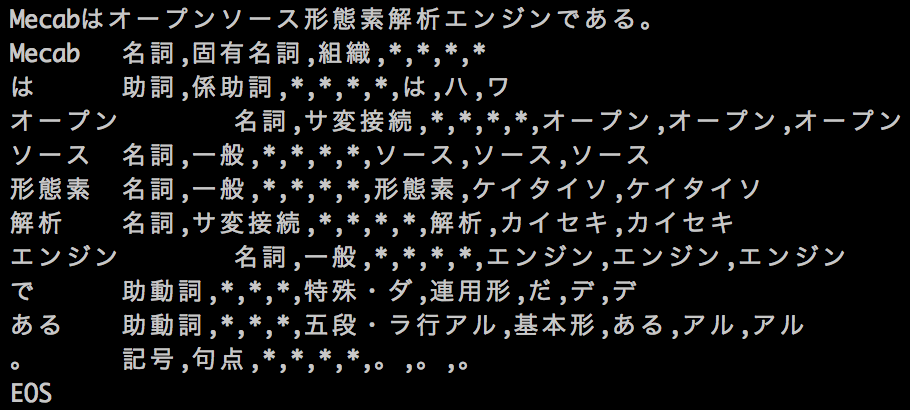
\includegraphics[width=\textwidth]{../images/4.Implementation/mecab.png}
  \caption{解析結果}
  \label{Fig:mecab}
  \vspace{-10pt}
 \end{center}
\end{figure}

出力フォーマットは次の形式となっている.\\
\ovalbox{表層形 \verb|\t| 品詞,品詞細分類1,品詞細分類2,品詞細分類3,活用型,活用形,原形,読み,発音}\\
「読み」と「発音」は図\ref{Fig:mecab}の"MeCab"のように不明であるものには付与されない.
MeCabによる形態素解析の結果,次の条件を満たす単語を除外している.
\begin{enumerate}
  \item 品詞細分類に「数」を含む
  \item 「読み」,「発音」が不明である
  \item 品詞が「助詞」,「助動詞」,「記号」,「連体詞」のどれかである. 
  \item 1文字のひらがなである
  \item 品詞細分類に「接尾」または「非自立」を含む
\end{enumerate}
上記の条件を満たす単語を除外したのは\ref{impl:preProcessing:weight}節で説明する重み付けにおいて重要な単語であると判定されやすいが,\ref{impl:preProcessing:sim}節で説明する類似度計算において精度を下げてしまうからである.
単語の除外は重み付けにおいて文章を単語に分割する際に行われる.

\subsection{重み付け}
\label{impl:preProcessing:weight}
提案手法では\ref{rel:part:weight}節で説明したokapiBM25とLexRankの2種類の重み付け手法をを統合して発言の内容の文字列$remark$中の単語に対して重み付けを行う.
アルゴリズムを\textbf{Algorithm\ref{algo:combinedWeight}}に示す.
\begin{algorithm}
\caption{統合重みの計算アルゴリズム} \label{algo:combinedWeight}
\begin{algorithmic}[1]
\State $Input: remark  ~ 発言内容の文字列$
\State $Output:  combinedWeight ~ remark中の単語と重みを対応付けた連想配列$
\State $Array ~~ sentList;$ \Comment{以前に重み付けを行ったm個前までの文章のリスト}
\Procedure{calcCombinedWeight}{$reamrk$} 
	\State bm25Weight = calcBM25Weight(remark)\Comment{単語と重みの連想配列}
	\For{Each$~ sent \in remark$}\Comment{remarkを句点,改行コードで分割する}
		\State sentList.append(sent)
	\EndFor
	\State lexWeight = calcLexRank(sentList)
	 \For{Each$~ word  \in bm25Weight.keys()$}\label{algo:combinedWight:for1-b}
	 	\State wordWeight = bm25Weight[word]
		\If{word is 固有名詞}
			\State wordWeight *=2\label{algo:combinedWight:pNoun}
		\EndIf
		\State sentWeight = 0
		\For{Each$~ sent \in remark$}\label{algo:combinedWight:for2-b}
			\If{word in sent}
				\State sentWeight+=lexWeight[sent]
			\EndIf
		\EndFor\label{algo:combinedWight:for2-e}
		\State combinedWeight[word] = wordWeight*sentWeight \label{algo:combinedWight:final}
	 \EndFor\label{algo:combinedWeight:for1-e}
	\State \textbf{return} combinedWeight
\EndProcedure
\end{algorithmic}
\end{algorithm}

固有名詞は文章の中で重要な役割を果たす可能性が大きいと考え,\ref{algo:combinedWight:pNoun}行目では固有名詞の単語重みを倍にしている.そして,\ref{algo:combinedWight:for2-b} $\sim$ \ref{algo:combinedWight:final}行目ではwordを含む全文章の重みの合計を求め,okapiBM25による単語重みを掛け合わせたものをwordの統合重みとしている.単語重みに単語を含む文章の重みを掛け合わせることで感嘆文のような文章そのものは重要でないが頻度の少ない単語を使用する文章中の単語が選ばれる可能性を下げている.
\section{類似度計算}
\label{impl:similarity}
\subsection{単語抽出}
\label{impl:similarity:extract}
\ref{impl:preProcessing}節で計算された単語重みの値が大きいものの上位n個までの単語を発言文章remarkにおいて重要度の高い単語であるとして抽出する.単語重みが等しいものが複数あった場合は単語を昇順に並び替えて順序を付けている.また,使用する分散表現モデルに登録されていない単語は除外している.
\subsection{分散表現による類似度計算}
\label{impl:similarity:wordEmbed}
\ref{impl:similarity:extract}節で述べた手法を用いて2発言それぞれから抽出した単語集合の類似度を分散表現を用いて求める.
それぞれの単語集合の単語ベクトルの平均を求め,\ref{rel:part:vec}の図\ref{eq:cosineSim}で述べたようにCosine類似度を2平均ベクトル間で取っている.
\section{結言}
\label{impl:conclusion}
本章では発言内容の類似度を計算する手法について説明した.文章を単語に分割する手法と使用したツールと単語を除外する前処理についても述べた.また,okapiBM25とLexRankを組み合わせた発言中の単語の重み付け手法,及び重み付けによって抽出した単語集合の類似度計算手法についても説明した.

 %-------------------------------------------------------------------------------
 \expandafter\ifx\csname MasterFile\endcsname\relax
	\def\BibFile{hoge}
	\expandafter\ifx\csname MasterFile\endcsname\relax
\def\SubFile{hoge}
\documentclass[a4j,12pt,twoside,openany]{jreport}
%\nofiles %tocファイルを更新させない
%\documentclass[12pt,a4j,twoside,openany]{jsbook}
\usepackage[dvipdfmx]{graphicx}
\usepackage{../dspc} % ベースラインスキップの指定
\usepackage{../slashbox} % 表に斜線を入れる
%\usepackage{../mediabb}
\usepackage{fancyvrb} % Verbatim環境
\usepackage{fancyhdr} % Headerの下線付き章見出し
\usepackage{here} % float[H]
\usepackage{multirow}
\usepackage{hhline} % 表の罫線の角を美しくする
\usepackage{amsmath} %コレがないとcasesが動かない
\usepackage{amsfonts} % 数学用フォント
\usepackage{bm} % 数式環境での bold
\usepackage{algorithm}
\usepackage{algorithmicx}
\usepackage[noend]{algpseudocode}%\procedureはここに含まれる
\usepackage[flushleft]{threeparttable} % 脚注付きテーブル
\usepackage{enumitem}
\usepackage{comment}
\usepackage{fancybox}
%\usepackage{csvsimple,booktabs,siunitx}
%\usepackage{filecontents}
\usepackage{ulinej}


\setlength{\evensidemargin}{5pt}
\setlength{\oddsidemargin}{40pt}
%\setlength{\headheight}{16.5pt}
%%\setlength{\headheight}{30pt}
\setcounter{secnumdepth}{3}
\setlist[description]{leftmargin=2\parindent,labelindent=\parindent}

\makeatletter
\def\@makechapterhead#1{%
	\vspace*{50\p@}%
	{
		\parindent \z@ \raggedright \normalfont
		\ifnum \c@secnumdepth >\m@ne
		% \if@mainmatter
			\huge\bfseries\@chapapp\thechapter\@chappos
			\par\nobreak
			\vskip 20\p@
		% \fi
		\fi
		\interlinepenalty\@M
		\Huge\bfseries #1\par\nobreak
		\vskip 40\p@
	}
}

%新しいコマンド定義
\newcounter{linenumber}
\newenvironment{listing}{%
  \begin{list}{%
    \small\arabic{linenumber}:}{%
      \usecounter{linenumber}%
      \setlength{\baselineskip}{18pt}%
      \setlength{\itemsep}{0pt}%
      \setlength{\parsep}{0pt}}}%
 {\end{list}}
\newcommand{\figcaption}[1]{\def\@captype{figure}\caption{#1}}
\newcommand{\tblcaption}[1]{\def\@captype{table}\caption{#1}}
\newcommand{\norm}[1]{\left\| #1 \right\|}
\newcommand{\cc}[1]{\multicolumn{1}{|c|}{#1}}
\newcommand{\circled}[1]{\raisebox{.5pt}{\textcircled{\raisebox{-.9pt} {#1}}}}
\newcommand{\specialcell}[2][c]{%
  \begin{tabular}[#1]{@{}c@{}}#2\end{tabular}}
\makeatother
%===============================================================================
\expandafter\ifx\csname SubFile\endcsname\relax
\begin{document}
\def\MasterFile{hoge}
%-------------------------------------------------------------------------------
%\maketitle
\thispagestyle{empty}
\documentclass[a4j,12pt]{jarticle}
% 外表紙

% 題名
\def\title{降水量予測のための\\Sequence-to-Sequenceモデルに基づく\\マルチモーダル学習}
% 著者
\def\author{林 政行}
% 入学年度(平成)
\def\year{24}
% 学籍番号
\def\number{24115113}
% 指導教官
\def\kyoukan{伊藤孝行}
% 指導教官役職
\def\kyoukanrank{教授}
% 提出日
\def\teisyutubi{平成28年2月8日}

\begin{document}
\pagestyle{empty}
\baselineskip=18pt

\begin{center}

\vspace*{2cm}

{\huge \textbf{卒業論文}}

\vspace*{3cm}

%\vrule width 10cm height 1pt depth 0pt



%(題目)
%\vspace{5pt}
%\hrule height 3pt
%\vspace{1zh}

\vrule width 6.25cm height 6pt depth -2pt
\makebox[1.5cm]{(題目)}
\vrule width 6.25cm height 6pt depth -2pt

{\LARGE {\title}}

\vspace{1zh}
%{\large {\subtitle}}
%\hrule height 3pt
\vrule width 14cm height 4pt depth 0pt

\vspace*{1cm}

指導教員 {\large {\kyoukan}} {\kyoukanrank}

%\vspace*{5cm}
\vfill

{\large 名古屋工業大学 情報工学科}

{\large 平成{\year}年度 入学 ({\number})}

\vspace*{1cm}

%{\huge\mc {\author}}

\underline{(氏名)\hspace{3zw}{\huge\mc {\author}}\hspace{3zw}}

\vspace*{1cm}

({\teisyutubi}提出)

\vspace{2cm}
\end{center}

\end{document}
\begin{titlepage}

% 題名
\def\title{分散表現を用いた\\話題変化判定}
% 補助題名
\def\subtitle{卒業論文}
% 著者
\def\author{芳野 魁}
% 入学年度(平成)
\def\year{29}
% 学籍番号
\def\number{26115162}
% 指導教官
\def\kyoukan{伊藤 孝行}
% 指導教官役職
\def\kyoukanrank{教授}
% 提出日
\def\teisyutubi{平成29年9月19日}

\pagestyle{empty}

\begin{center}

\vspace*{20mm}
{\Large\mc 平成29年度 \hspace{7mm} 卒 業 論 文}
\vspace{15mm}

%\setlength{\unitlength}{1mm}
\begin{picture}(100,60)
  \put(0,0){\makebox(100,60){\huge\bf\shortstack{\title}}}
\end{picture}
\\
%\begin{picture}(100,5)
%  \put(0,0){\makebox(100,5){\Large\bf\shortstack{\subtitle}}}
%\end{picture}
\end{center}
\vspace{10mm}
\begin{flushright}
\begin{tabular}{ll}
{\large 提出日} & {\large {\teisyutubi}} \\
{\large 所属}  & {\large 名古屋工業大学 情報工学科} \\
{\large 指導教員} & {\large {\kyoukan} {\kyoukanrank}} \\
 & \\
{\large 入学年度} & {\large 平成{\year}年度入学}\\
{\large 学籍番号} &{\large {\number}} \\
 & \\
%{\large 氏名} & {\huge {\author}}
{\large 氏名} & {\huge\mc {\author}}
\end{tabular}
\end{flushright}

\end{titlepage}

%\addcontentsline{toc}{chapter}{表紙}
\thispagestyle{empty}
\mbox{}\newpage
%===============================================================================
%\frontmatter
%===============================================================================
%\mainmatter
%-------------------------------------------------------------------------------
\pagenumbering{arabic}
\cleardoublepage
\expandafter\ifx\csname MasterFile\endcsname\relax
\def\SubFile{hoge}
\input{../thesis/thesis}
\begin{document}
\fi
%-------------------------------------------------------------------------------
\cleardoublepage
\chapter*{論文要旨}\addcontentsline{toc}{chapter}{論文要旨}
近年,Web上での大規模な議論活動が活発になっているが,現在一般的に使われている "2ちゃんねる" や "Twitter" といったシステムでは整理や収束を行うことが困難である.困難である原因として,議論の管理を行う者がいないことが挙げられる.
議論を収束させるには議論のマネジメントを行う人物が必要である.
%
大規模意見集約システムCOLLAGREEではファシリテーターと呼ばれる人物が議論のマネジメントを行っている.
しかし,ファシリテーターは人間であり,長時間に渡って大人数での議論の動向をマネジメントし続けるのは困難である.
%
COLLAGREEで大規模な議論を収束させるためには,ファシリテーターが必要な時にだけ画面を見るようにして画面に向き合う時間を減らす工夫があることが望ましい.ファシリテーターが画面を見るべきタイミングは議論の話題が変化したときである.以前の議論の内容から外れた発言がされた時,ファシリテーターが適切に発言することで,脱線や炎上を避けて議論を収束させることができる.
すなわち,ファシリテーターの代わりに自動的に議論中の話題の変化を事前に判定することが求められている.
%
現在,COLLAGREE上で使用されている議論支援システムは投稿支援システムと議論可視化システムの2つに大別できる.
投稿支援システムはポイント機能やファシリテーションフレーズ簡易投稿機能のように,ユーザーが投稿をする際に何らかの補助やリアクションを行う.現行の機能では選択肢の提示に留まっており,作業量を減らすことには繋がりにくい。
一方,議論可視化システムは議論ツリーやキーワード抽出のように,ユーザーにスレッドとは異なる議論の見方を提供する.現行の機能では議論を見やすくすることに重点が置かれており,議論の把握の助けにはなるが画面に向き合う時間を減らすことにはなりにくい.むしろ,作業量を増やすことになり得る機能もある.
\begin{comment}
ポイント機能(ユーザの議論行動を活性化)-1
ファシリテーションフレーズ簡易投稿機能-1
議論ツリー-2
1文の要約,スレッドの要約,クラスタリング,返信意見の極性判定-2
ファシリテーションスタンプ-1
キーワード抽出-2
いいね機能-1
いいねランキング-2
投票機能-1
議論フェーズ機能-2
1-意見を出す、投稿をする際に補助や選択肢、リアクションを与える
2-議論の別の見方を提供する
\end{comment}
%
近年,自然言語処理の分野において分散表現が多くの研究で使われており,機械翻訳を始めとする単語の意味が重要となる分野で精度の向上が確認されている.分散表現を用いることで,人間に近い精度で話題の変化を観測することが可能となる.
%
以上のような背景を踏まえて,分散表現を用いて,話題の変化を観測し,話題の変化が確認された時にファシリテーターに伝えることが望ましい.
話題の変化の観測は,発言中に現れる単語の関連度合いの計算と見なすことができる.
分散表現を用いることで単語間の類似度を求めることができる,値が大きいほど単語がそれぞれ類似した実数ベクトルであることを表す.単語Aと単語Bの実数ベクトルが類似しているとは,単語Aと共に使われることの多い単語と単語Bと共に使われることの多い単語が多く共通していることを示す.故に,分散表現を使って単語の関連度を計算することができる.
%
発言文から単語を選ぶ際には自動要約を用いる.発言文から重要でない単語を取り除くことで関連度の計算の精度を高めることが可能となる.
%
本論文では,分散表現を用いて議論中での発言に含まれる単語の関連度を計算し,話題の変化を観測する手法を提案する.
%
提案手法は,既存の抽出的要約手法を用いて選ばれた単語の関連度を計算する手法,Seq2Seqによる生成的要約を用いて生成された単語の関連度を計算する手法,オントロジーを用いて求められた単語の関連度を計算する手法の3つである.
提案した3つの手法により,議論中の話題の変化の観測の評価実験を行い,各手法の評価を行う.
評価実験によって,提案手法を用いることで人間の代わりに自動的に話題の変化を観測できることを確認する.
%
 \begin{comment}
大規模な議論では意見を共有することは可能であるが,議論を整理させることや収束させることは難しい.以上から大規模意見集約システムCOLLAGREEが開発された.本システムではWeb上で適切に大規模な議論を行うことができるように議論をマネジメントするファシリテーターを導入した.
過去の実験ではファシリテーターの存在が議論の集約に大きな役割を果たしていることが認識されており,大規模な議論のためにファシリテータは必要である.しかし,議論の規模に伴って議論時間が長くなる傾向があり,同時にファシリテーターは常に議論の動向を見続ける必要がある.故に,議論の規模が大きくなればなるほどファシリテーターは長時間かつ大規模な議論の動向の監視によって大きな負担がかかる.大規模な議論が増加する傾向を踏まえるとファシリテーターにかかる負担を軽減する支援が必要となることは明白である.
また,近年自然言語処理の分野において分散表現が多くの研究で使われており,機械翻訳を始めとする複数の分野で精度の向上が確認されている.まだ適応されていない分野でも結果の向上が期待できる.
従って,本研究では負担軽減の1つとして分散表現を用いて議論中での話題の変化を人間の代わりに検知することでファシリテーターの負担を軽減することを目指す.
-----------------

\end{comment}
%-------------------------------------------------------------------------------
\expandafter\ifx\csname MasterFile\endcsname\relax
\end{document}
\fi

%-------------------------------------------------------------------------------
\clearpage
\addcontentsline{toc}{chapter}{目次}
\tableofcontents

\clearpage
\addcontentsline{toc}{chapter}{図目次}
\listoffigures

\clearpage
\addcontentsline{toc}{chapter}{表目次}
\listoftables

%-------------------------------------------------------------------------------

%=====================
\pagestyle{fancy} % Headerをつける
\renewcommand{\sectionmark}[1]{\markright{\thesection\ \ \ #1}}
\renewcommand{\chaptermark}[1]{\markboth{#1}{}}
\lhead{}
\chead{}
\lfoot{}
\rfoot{}%-------------------------------------------------------------------------------
\expandafter\ifx\csname MasterFile\endcsname\relax
\def\SubFile{hoge}
\input{../thesis/thesis}
\begin{document}
\fi
%-------------------------------------------------------------------------------
\cleardoublepage
\chapter*{論文要旨}\addcontentsline{toc}{chapter}{論文要旨}
近年,Web上での大規模な議論活動が活発になっているが,現在一般的に使われている "2ちゃんねる" や "Twitter" といったシステムでは整理や収束を行うことが困難である.困難である原因として,議論の管理を行う者がいないことが挙げられる.
議論を収束させるには議論のマネジメントを行う人物が必要である.
%
大規模意見集約システムCOLLAGREEではファシリテーターと呼ばれる人物が議論のマネジメントを行っている.
しかし,ファシリテーターは人間であり,長時間に渡って大人数での議論の動向をマネジメントし続けるのは困難である.
%
COLLAGREEで大規模な議論を収束させるためには,ファシリテーターが必要な時にだけ画面を見るようにして画面に向き合う時間を減らす工夫があることが望ましい.ファシリテーターが画面を見るべきタイミングは議論の話題が変化したときである.以前の議論の内容から外れた発言がされた時,ファシリテーターが適切に発言することで,脱線や炎上を避けて議論を収束させることができる.
すなわち,ファシリテーターの代わりに自動的に議論中の話題の変化を事前に判定することが求められている.
%
現在,COLLAGREE上で使用されている議論支援システムは投稿支援システムと議論可視化システムの2つに大別できる.
投稿支援システムはポイント機能やファシリテーションフレーズ簡易投稿機能のように,ユーザーが投稿をする際に何らかの補助やリアクションを行う.現行の機能では選択肢の提示に留まっており,作業量を減らすことには繋がりにくい。
一方,議論可視化システムは議論ツリーやキーワード抽出のように,ユーザーにスレッドとは異なる議論の見方を提供する.現行の機能では議論を見やすくすることに重点が置かれており,議論の把握の助けにはなるが画面に向き合う時間を減らすことにはなりにくい.むしろ,作業量を増やすことになり得る機能もある.
\begin{comment}
ポイント機能(ユーザの議論行動を活性化)-1
ファシリテーションフレーズ簡易投稿機能-1
議論ツリー-2
1文の要約,スレッドの要約,クラスタリング,返信意見の極性判定-2
ファシリテーションスタンプ-1
キーワード抽出-2
いいね機能-1
いいねランキング-2
投票機能-1
議論フェーズ機能-2
1-意見を出す、投稿をする際に補助や選択肢、リアクションを与える
2-議論の別の見方を提供する
\end{comment}
%
近年,自然言語処理の分野において分散表現が多くの研究で使われており,機械翻訳を始めとする単語の意味が重要となる分野で精度の向上が確認されている.分散表現を用いることで,人間に近い精度で話題の変化を観測することが可能となる.
%
以上のような背景を踏まえて,分散表現を用いて,話題の変化を観測し,話題の変化が確認された時にファシリテーターに伝えることが望ましい.
話題の変化の観測は,発言中に現れる単語の関連度合いの計算と見なすことができる.
分散表現を用いることで単語間の類似度を求めることができる,値が大きいほど単語がそれぞれ類似した実数ベクトルであることを表す.単語Aと単語Bの実数ベクトルが類似しているとは,単語Aと共に使われることの多い単語と単語Bと共に使われることの多い単語が多く共通していることを示す.故に,分散表現を使って単語の関連度を計算することができる.
%
発言文から単語を選ぶ際には自動要約を用いる.発言文から重要でない単語を取り除くことで関連度の計算の精度を高めることが可能となる.
%
本論文では,分散表現を用いて議論中での発言に含まれる単語の関連度を計算し,話題の変化を観測する手法を提案する.
%
提案手法は,既存の抽出的要約手法を用いて選ばれた単語の関連度を計算する手法,Seq2Seqによる生成的要約を用いて生成された単語の関連度を計算する手法,オントロジーを用いて求められた単語の関連度を計算する手法の3つである.
提案した3つの手法により,議論中の話題の変化の観測の評価実験を行い,各手法の評価を行う.
評価実験によって,提案手法を用いることで人間の代わりに自動的に話題の変化を観測できることを確認する.
%
 \begin{comment}
大規模な議論では意見を共有することは可能であるが,議論を整理させることや収束させることは難しい.以上から大規模意見集約システムCOLLAGREEが開発された.本システムではWeb上で適切に大規模な議論を行うことができるように議論をマネジメントするファシリテーターを導入した.
過去の実験ではファシリテーターの存在が議論の集約に大きな役割を果たしていることが認識されており,大規模な議論のためにファシリテータは必要である.しかし,議論の規模に伴って議論時間が長くなる傾向があり,同時にファシリテーターは常に議論の動向を見続ける必要がある.故に,議論の規模が大きくなればなるほどファシリテーターは長時間かつ大規模な議論の動向の監視によって大きな負担がかかる.大規模な議論が増加する傾向を踏まえるとファシリテーターにかかる負担を軽減する支援が必要となることは明白である.
また,近年自然言語処理の分野において分散表現が多くの研究で使われており,機械翻訳を始めとする複数の分野で精度の向上が確認されている.まだ適応されていない分野でも結果の向上が期待できる.
従って,本研究では負担軽減の1つとして分散表現を用いて議論中での話題の変化を人間の代わりに検知することでファシリテーターの負担を軽減することを目指す.
-----------------

\end{comment}
%-------------------------------------------------------------------------------
\expandafter\ifx\csname MasterFile\endcsname\relax
\end{document}
\fi

%-------------------------------------------------------------------------------
\expandafter\ifx\csname MasterFile\endcsname\relax
\def\SubFile{hoge}
\input{../thesis/thesis}
\begin{document}
\fi
%-------------------------------------------------------------------------------
\cleardoublepage
\chapter*{論文要旨}\addcontentsline{toc}{chapter}{論文要旨}
近年,Web上での大規模な議論活動が活発になっているが,現在一般的に使われている "2ちゃんねる" や "Twitter" といったシステムでは整理や収束を行うことが困難である.困難である原因として,議論の管理を行う者がいないことが挙げられる.
議論を収束させるには議論のマネジメントを行う人物が必要である.
%
大規模意見集約システムCOLLAGREEではファシリテーターと呼ばれる人物が議論のマネジメントを行っている.
しかし,ファシリテーターは人間であり,長時間に渡って大人数での議論の動向をマネジメントし続けるのは困難である.
%
COLLAGREEで大規模な議論を収束させるためには,ファシリテーターが必要な時にだけ画面を見るようにして画面に向き合う時間を減らす工夫があることが望ましい.ファシリテーターが画面を見るべきタイミングは議論の話題が変化したときである.以前の議論の内容から外れた発言がされた時,ファシリテーターが適切に発言することで,脱線や炎上を避けて議論を収束させることができる.
すなわち,ファシリテーターの代わりに自動的に議論中の話題の変化を事前に判定することが求められている.
%
現在,COLLAGREE上で使用されている議論支援システムは投稿支援システムと議論可視化システムの2つに大別できる.
投稿支援システムはポイント機能やファシリテーションフレーズ簡易投稿機能のように,ユーザーが投稿をする際に何らかの補助やリアクションを行う.現行の機能では選択肢の提示に留まっており,作業量を減らすことには繋がりにくい。
一方,議論可視化システムは議論ツリーやキーワード抽出のように,ユーザーにスレッドとは異なる議論の見方を提供する.現行の機能では議論を見やすくすることに重点が置かれており,議論の把握の助けにはなるが画面に向き合う時間を減らすことにはなりにくい.むしろ,作業量を増やすことになり得る機能もある.
\begin{comment}
ポイント機能(ユーザの議論行動を活性化)-1
ファシリテーションフレーズ簡易投稿機能-1
議論ツリー-2
1文の要約,スレッドの要約,クラスタリング,返信意見の極性判定-2
ファシリテーションスタンプ-1
キーワード抽出-2
いいね機能-1
いいねランキング-2
投票機能-1
議論フェーズ機能-2
1-意見を出す、投稿をする際に補助や選択肢、リアクションを与える
2-議論の別の見方を提供する
\end{comment}
%
近年,自然言語処理の分野において分散表現が多くの研究で使われており,機械翻訳を始めとする単語の意味が重要となる分野で精度の向上が確認されている.分散表現を用いることで,人間に近い精度で話題の変化を観測することが可能となる.
%
以上のような背景を踏まえて,分散表現を用いて,話題の変化を観測し,話題の変化が確認された時にファシリテーターに伝えることが望ましい.
話題の変化の観測は,発言中に現れる単語の関連度合いの計算と見なすことができる.
分散表現を用いることで単語間の類似度を求めることができる,値が大きいほど単語がそれぞれ類似した実数ベクトルであることを表す.単語Aと単語Bの実数ベクトルが類似しているとは,単語Aと共に使われることの多い単語と単語Bと共に使われることの多い単語が多く共通していることを示す.故に,分散表現を使って単語の関連度を計算することができる.
%
発言文から単語を選ぶ際には自動要約を用いる.発言文から重要でない単語を取り除くことで関連度の計算の精度を高めることが可能となる.
%
本論文では,分散表現を用いて議論中での発言に含まれる単語の関連度を計算し,話題の変化を観測する手法を提案する.
%
提案手法は,既存の抽出的要約手法を用いて選ばれた単語の関連度を計算する手法,Seq2Seqによる生成的要約を用いて生成された単語の関連度を計算する手法,オントロジーを用いて求められた単語の関連度を計算する手法の3つである.
提案した3つの手法により,議論中の話題の変化の観測の評価実験を行い,各手法の評価を行う.
評価実験によって,提案手法を用いることで人間の代わりに自動的に話題の変化を観測できることを確認する.
%
 \begin{comment}
大規模な議論では意見を共有することは可能であるが,議論を整理させることや収束させることは難しい.以上から大規模意見集約システムCOLLAGREEが開発された.本システムではWeb上で適切に大規模な議論を行うことができるように議論をマネジメントするファシリテーターを導入した.
過去の実験ではファシリテーターの存在が議論の集約に大きな役割を果たしていることが認識されており,大規模な議論のためにファシリテータは必要である.しかし,議論の規模に伴って議論時間が長くなる傾向があり,同時にファシリテーターは常に議論の動向を見続ける必要がある.故に,議論の規模が大きくなればなるほどファシリテーターは長時間かつ大規模な議論の動向の監視によって大きな負担がかかる.大規模な議論が増加する傾向を踏まえるとファシリテーターにかかる負担を軽減する支援が必要となることは明白である.
また,近年自然言語処理の分野において分散表現が多くの研究で使われており,機械翻訳を始めとする複数の分野で精度の向上が確認されている.まだ適応されていない分野でも結果の向上が期待できる.
従って,本研究では負担軽減の1つとして分散表現を用いて議論中での話題の変化を人間の代わりに検知することでファシリテーターの負担を軽減することを目指す.
-----------------

\end{comment}
%-------------------------------------------------------------------------------
\expandafter\ifx\csname MasterFile\endcsname\relax
\end{document}
\fi

%-------------------------------------------------------------------------------
\expandafter\ifx\csname MasterFile\endcsname\relax
\def\SubFile{hoge}
\input{../thesis/thesis}
\begin{document}
\fi
%-------------------------------------------------------------------------------
\cleardoublepage
\chapter*{論文要旨}\addcontentsline{toc}{chapter}{論文要旨}
近年,Web上での大規模な議論活動が活発になっているが,現在一般的に使われている "2ちゃんねる" や "Twitter" といったシステムでは整理や収束を行うことが困難である.困難である原因として,議論の管理を行う者がいないことが挙げられる.
議論を収束させるには議論のマネジメントを行う人物が必要である.
%
大規模意見集約システムCOLLAGREEではファシリテーターと呼ばれる人物が議論のマネジメントを行っている.
しかし,ファシリテーターは人間であり,長時間に渡って大人数での議論の動向をマネジメントし続けるのは困難である.
%
COLLAGREEで大規模な議論を収束させるためには,ファシリテーターが必要な時にだけ画面を見るようにして画面に向き合う時間を減らす工夫があることが望ましい.ファシリテーターが画面を見るべきタイミングは議論の話題が変化したときである.以前の議論の内容から外れた発言がされた時,ファシリテーターが適切に発言することで,脱線や炎上を避けて議論を収束させることができる.
すなわち,ファシリテーターの代わりに自動的に議論中の話題の変化を事前に判定することが求められている.
%
現在,COLLAGREE上で使用されている議論支援システムは投稿支援システムと議論可視化システムの2つに大別できる.
投稿支援システムはポイント機能やファシリテーションフレーズ簡易投稿機能のように,ユーザーが投稿をする際に何らかの補助やリアクションを行う.現行の機能では選択肢の提示に留まっており,作業量を減らすことには繋がりにくい。
一方,議論可視化システムは議論ツリーやキーワード抽出のように,ユーザーにスレッドとは異なる議論の見方を提供する.現行の機能では議論を見やすくすることに重点が置かれており,議論の把握の助けにはなるが画面に向き合う時間を減らすことにはなりにくい.むしろ,作業量を増やすことになり得る機能もある.
\begin{comment}
ポイント機能(ユーザの議論行動を活性化)-1
ファシリテーションフレーズ簡易投稿機能-1
議論ツリー-2
1文の要約,スレッドの要約,クラスタリング,返信意見の極性判定-2
ファシリテーションスタンプ-1
キーワード抽出-2
いいね機能-1
いいねランキング-2
投票機能-1
議論フェーズ機能-2
1-意見を出す、投稿をする際に補助や選択肢、リアクションを与える
2-議論の別の見方を提供する
\end{comment}
%
近年,自然言語処理の分野において分散表現が多くの研究で使われており,機械翻訳を始めとする単語の意味が重要となる分野で精度の向上が確認されている.分散表現を用いることで,人間に近い精度で話題の変化を観測することが可能となる.
%
以上のような背景を踏まえて,分散表現を用いて,話題の変化を観測し,話題の変化が確認された時にファシリテーターに伝えることが望ましい.
話題の変化の観測は,発言中に現れる単語の関連度合いの計算と見なすことができる.
分散表現を用いることで単語間の類似度を求めることができる,値が大きいほど単語がそれぞれ類似した実数ベクトルであることを表す.単語Aと単語Bの実数ベクトルが類似しているとは,単語Aと共に使われることの多い単語と単語Bと共に使われることの多い単語が多く共通していることを示す.故に,分散表現を使って単語の関連度を計算することができる.
%
発言文から単語を選ぶ際には自動要約を用いる.発言文から重要でない単語を取り除くことで関連度の計算の精度を高めることが可能となる.
%
本論文では,分散表現を用いて議論中での発言に含まれる単語の関連度を計算し,話題の変化を観測する手法を提案する.
%
提案手法は,既存の抽出的要約手法を用いて選ばれた単語の関連度を計算する手法,Seq2Seqによる生成的要約を用いて生成された単語の関連度を計算する手法,オントロジーを用いて求められた単語の関連度を計算する手法の3つである.
提案した3つの手法により,議論中の話題の変化の観測の評価実験を行い,各手法の評価を行う.
評価実験によって,提案手法を用いることで人間の代わりに自動的に話題の変化を観測できることを確認する.
%
 \begin{comment}
大規模な議論では意見を共有することは可能であるが,議論を整理させることや収束させることは難しい.以上から大規模意見集約システムCOLLAGREEが開発された.本システムではWeb上で適切に大規模な議論を行うことができるように議論をマネジメントするファシリテーターを導入した.
過去の実験ではファシリテーターの存在が議論の集約に大きな役割を果たしていることが認識されており,大規模な議論のためにファシリテータは必要である.しかし,議論の規模に伴って議論時間が長くなる傾向があり,同時にファシリテーターは常に議論の動向を見続ける必要がある.故に,議論の規模が大きくなればなるほどファシリテーターは長時間かつ大規模な議論の動向の監視によって大きな負担がかかる.大規模な議論が増加する傾向を踏まえるとファシリテーターにかかる負担を軽減する支援が必要となることは明白である.
また,近年自然言語処理の分野において分散表現が多くの研究で使われており,機械翻訳を始めとする複数の分野で精度の向上が確認されている.まだ適応されていない分野でも結果の向上が期待できる.
従って,本研究では負担軽減の1つとして分散表現を用いて議論中での話題の変化を人間の代わりに検知することでファシリテーターの負担を軽減することを目指す.
-----------------

\end{comment}
%-------------------------------------------------------------------------------
\expandafter\ifx\csname MasterFile\endcsname\relax
\end{document}
\fi

%-------------------------------------------------------------------------------
\expandafter\ifx\csname MasterFile\endcsname\relax
\def\SubFile{hoge}
\input{../thesis/thesis}
\begin{document}
\fi
%-------------------------------------------------------------------------------
\cleardoublepage
\chapter*{論文要旨}\addcontentsline{toc}{chapter}{論文要旨}
近年,Web上での大規模な議論活動が活発になっているが,現在一般的に使われている "2ちゃんねる" や "Twitter" といったシステムでは整理や収束を行うことが困難である.困難である原因として,議論の管理を行う者がいないことが挙げられる.
議論を収束させるには議論のマネジメントを行う人物が必要である.
%
大規模意見集約システムCOLLAGREEではファシリテーターと呼ばれる人物が議論のマネジメントを行っている.
しかし,ファシリテーターは人間であり,長時間に渡って大人数での議論の動向をマネジメントし続けるのは困難である.
%
COLLAGREEで大規模な議論を収束させるためには,ファシリテーターが必要な時にだけ画面を見るようにして画面に向き合う時間を減らす工夫があることが望ましい.ファシリテーターが画面を見るべきタイミングは議論の話題が変化したときである.以前の議論の内容から外れた発言がされた時,ファシリテーターが適切に発言することで,脱線や炎上を避けて議論を収束させることができる.
すなわち,ファシリテーターの代わりに自動的に議論中の話題の変化を事前に判定することが求められている.
%
現在,COLLAGREE上で使用されている議論支援システムは投稿支援システムと議論可視化システムの2つに大別できる.
投稿支援システムはポイント機能やファシリテーションフレーズ簡易投稿機能のように,ユーザーが投稿をする際に何らかの補助やリアクションを行う.現行の機能では選択肢の提示に留まっており,作業量を減らすことには繋がりにくい。
一方,議論可視化システムは議論ツリーやキーワード抽出のように,ユーザーにスレッドとは異なる議論の見方を提供する.現行の機能では議論を見やすくすることに重点が置かれており,議論の把握の助けにはなるが画面に向き合う時間を減らすことにはなりにくい.むしろ,作業量を増やすことになり得る機能もある.
\begin{comment}
ポイント機能(ユーザの議論行動を活性化)-1
ファシリテーションフレーズ簡易投稿機能-1
議論ツリー-2
1文の要約,スレッドの要約,クラスタリング,返信意見の極性判定-2
ファシリテーションスタンプ-1
キーワード抽出-2
いいね機能-1
いいねランキング-2
投票機能-1
議論フェーズ機能-2
1-意見を出す、投稿をする際に補助や選択肢、リアクションを与える
2-議論の別の見方を提供する
\end{comment}
%
近年,自然言語処理の分野において分散表現が多くの研究で使われており,機械翻訳を始めとする単語の意味が重要となる分野で精度の向上が確認されている.分散表現を用いることで,人間に近い精度で話題の変化を観測することが可能となる.
%
以上のような背景を踏まえて,分散表現を用いて,話題の変化を観測し,話題の変化が確認された時にファシリテーターに伝えることが望ましい.
話題の変化の観測は,発言中に現れる単語の関連度合いの計算と見なすことができる.
分散表現を用いることで単語間の類似度を求めることができる,値が大きいほど単語がそれぞれ類似した実数ベクトルであることを表す.単語Aと単語Bの実数ベクトルが類似しているとは,単語Aと共に使われることの多い単語と単語Bと共に使われることの多い単語が多く共通していることを示す.故に,分散表現を使って単語の関連度を計算することができる.
%
発言文から単語を選ぶ際には自動要約を用いる.発言文から重要でない単語を取り除くことで関連度の計算の精度を高めることが可能となる.
%
本論文では,分散表現を用いて議論中での発言に含まれる単語の関連度を計算し,話題の変化を観測する手法を提案する.
%
提案手法は,既存の抽出的要約手法を用いて選ばれた単語の関連度を計算する手法,Seq2Seqによる生成的要約を用いて生成された単語の関連度を計算する手法,オントロジーを用いて求められた単語の関連度を計算する手法の3つである.
提案した3つの手法により,議論中の話題の変化の観測の評価実験を行い,各手法の評価を行う.
評価実験によって,提案手法を用いることで人間の代わりに自動的に話題の変化を観測できることを確認する.
%
 \begin{comment}
大規模な議論では意見を共有することは可能であるが,議論を整理させることや収束させることは難しい.以上から大規模意見集約システムCOLLAGREEが開発された.本システムではWeb上で適切に大規模な議論を行うことができるように議論をマネジメントするファシリテーターを導入した.
過去の実験ではファシリテーターの存在が議論の集約に大きな役割を果たしていることが認識されており,大規模な議論のためにファシリテータは必要である.しかし,議論の規模に伴って議論時間が長くなる傾向があり,同時にファシリテーターは常に議論の動向を見続ける必要がある.故に,議論の規模が大きくなればなるほどファシリテーターは長時間かつ大規模な議論の動向の監視によって大きな負担がかかる.大規模な議論が増加する傾向を踏まえるとファシリテーターにかかる負担を軽減する支援が必要となることは明白である.
また,近年自然言語処理の分野において分散表現が多くの研究で使われており,機械翻訳を始めとする複数の分野で精度の向上が確認されている.まだ適応されていない分野でも結果の向上が期待できる.
従って,本研究では負担軽減の1つとして分散表現を用いて議論中での話題の変化を人間の代わりに検知することでファシリテーターの負担を軽減することを目指す.
-----------------

\end{comment}
%-------------------------------------------------------------------------------
\expandafter\ifx\csname MasterFile\endcsname\relax
\end{document}
\fi

%-------------------------------------------------------------------------------
\expandafter\ifx\csname MasterFile\endcsname\relax
\def\SubFile{hoge}
\input{../thesis/thesis}
\begin{document}
\fi
%-------------------------------------------------------------------------------
\cleardoublepage
\chapter*{論文要旨}\addcontentsline{toc}{chapter}{論文要旨}
近年,Web上での大規模な議論活動が活発になっているが,現在一般的に使われている "2ちゃんねる" や "Twitter" といったシステムでは整理や収束を行うことが困難である.困難である原因として,議論の管理を行う者がいないことが挙げられる.
議論を収束させるには議論のマネジメントを行う人物が必要である.
%
大規模意見集約システムCOLLAGREEではファシリテーターと呼ばれる人物が議論のマネジメントを行っている.
しかし,ファシリテーターは人間であり,長時間に渡って大人数での議論の動向をマネジメントし続けるのは困難である.
%
COLLAGREEで大規模な議論を収束させるためには,ファシリテーターが必要な時にだけ画面を見るようにして画面に向き合う時間を減らす工夫があることが望ましい.ファシリテーターが画面を見るべきタイミングは議論の話題が変化したときである.以前の議論の内容から外れた発言がされた時,ファシリテーターが適切に発言することで,脱線や炎上を避けて議論を収束させることができる.
すなわち,ファシリテーターの代わりに自動的に議論中の話題の変化を事前に判定することが求められている.
%
現在,COLLAGREE上で使用されている議論支援システムは投稿支援システムと議論可視化システムの2つに大別できる.
投稿支援システムはポイント機能やファシリテーションフレーズ簡易投稿機能のように,ユーザーが投稿をする際に何らかの補助やリアクションを行う.現行の機能では選択肢の提示に留まっており,作業量を減らすことには繋がりにくい。
一方,議論可視化システムは議論ツリーやキーワード抽出のように,ユーザーにスレッドとは異なる議論の見方を提供する.現行の機能では議論を見やすくすることに重点が置かれており,議論の把握の助けにはなるが画面に向き合う時間を減らすことにはなりにくい.むしろ,作業量を増やすことになり得る機能もある.
\begin{comment}
ポイント機能(ユーザの議論行動を活性化)-1
ファシリテーションフレーズ簡易投稿機能-1
議論ツリー-2
1文の要約,スレッドの要約,クラスタリング,返信意見の極性判定-2
ファシリテーションスタンプ-1
キーワード抽出-2
いいね機能-1
いいねランキング-2
投票機能-1
議論フェーズ機能-2
1-意見を出す、投稿をする際に補助や選択肢、リアクションを与える
2-議論の別の見方を提供する
\end{comment}
%
近年,自然言語処理の分野において分散表現が多くの研究で使われており,機械翻訳を始めとする単語の意味が重要となる分野で精度の向上が確認されている.分散表現を用いることで,人間に近い精度で話題の変化を観測することが可能となる.
%
以上のような背景を踏まえて,分散表現を用いて,話題の変化を観測し,話題の変化が確認された時にファシリテーターに伝えることが望ましい.
話題の変化の観測は,発言中に現れる単語の関連度合いの計算と見なすことができる.
分散表現を用いることで単語間の類似度を求めることができる,値が大きいほど単語がそれぞれ類似した実数ベクトルであることを表す.単語Aと単語Bの実数ベクトルが類似しているとは,単語Aと共に使われることの多い単語と単語Bと共に使われることの多い単語が多く共通していることを示す.故に,分散表現を使って単語の関連度を計算することができる.
%
発言文から単語を選ぶ際には自動要約を用いる.発言文から重要でない単語を取り除くことで関連度の計算の精度を高めることが可能となる.
%
本論文では,分散表現を用いて議論中での発言に含まれる単語の関連度を計算し,話題の変化を観測する手法を提案する.
%
提案手法は,既存の抽出的要約手法を用いて選ばれた単語の関連度を計算する手法,Seq2Seqによる生成的要約を用いて生成された単語の関連度を計算する手法,オントロジーを用いて求められた単語の関連度を計算する手法の3つである.
提案した3つの手法により,議論中の話題の変化の観測の評価実験を行い,各手法の評価を行う.
評価実験によって,提案手法を用いることで人間の代わりに自動的に話題の変化を観測できることを確認する.
%
 \begin{comment}
大規模な議論では意見を共有することは可能であるが,議論を整理させることや収束させることは難しい.以上から大規模意見集約システムCOLLAGREEが開発された.本システムではWeb上で適切に大規模な議論を行うことができるように議論をマネジメントするファシリテーターを導入した.
過去の実験ではファシリテーターの存在が議論の集約に大きな役割を果たしていることが認識されており,大規模な議論のためにファシリテータは必要である.しかし,議論の規模に伴って議論時間が長くなる傾向があり,同時にファシリテーターは常に議論の動向を見続ける必要がある.故に,議論の規模が大きくなればなるほどファシリテーターは長時間かつ大規模な議論の動向の監視によって大きな負担がかかる.大規模な議論が増加する傾向を踏まえるとファシリテーターにかかる負担を軽減する支援が必要となることは明白である.
また,近年自然言語処理の分野において分散表現が多くの研究で使われており,機械翻訳を始めとする複数の分野で精度の向上が確認されている.まだ適応されていない分野でも結果の向上が期待できる.
従って,本研究では負担軽減の1つとして分散表現を用いて議論中での話題の変化を人間の代わりに検知することでファシリテーターの負担を軽減することを目指す.
-----------------

\end{comment}
%-------------------------------------------------------------------------------
\expandafter\ifx\csname MasterFile\endcsname\relax
\end{document}
\fi

%-------------------------------------------------------------------------------
\expandafter\ifx\csname MasterFile\endcsname\relax
\def\SubFile{hoge}
\input{../thesis/thesis}
\begin{document}
\fi
%-------------------------------------------------------------------------------
\cleardoublepage
\chapter*{論文要旨}\addcontentsline{toc}{chapter}{論文要旨}
近年,Web上での大規模な議論活動が活発になっているが,現在一般的に使われている "2ちゃんねる" や "Twitter" といったシステムでは整理や収束を行うことが困難である.困難である原因として,議論の管理を行う者がいないことが挙げられる.
議論を収束させるには議論のマネジメントを行う人物が必要である.
%
大規模意見集約システムCOLLAGREEではファシリテーターと呼ばれる人物が議論のマネジメントを行っている.
しかし,ファシリテーターは人間であり,長時間に渡って大人数での議論の動向をマネジメントし続けるのは困難である.
%
COLLAGREEで大規模な議論を収束させるためには,ファシリテーターが必要な時にだけ画面を見るようにして画面に向き合う時間を減らす工夫があることが望ましい.ファシリテーターが画面を見るべきタイミングは議論の話題が変化したときである.以前の議論の内容から外れた発言がされた時,ファシリテーターが適切に発言することで,脱線や炎上を避けて議論を収束させることができる.
すなわち,ファシリテーターの代わりに自動的に議論中の話題の変化を事前に判定することが求められている.
%
現在,COLLAGREE上で使用されている議論支援システムは投稿支援システムと議論可視化システムの2つに大別できる.
投稿支援システムはポイント機能やファシリテーションフレーズ簡易投稿機能のように,ユーザーが投稿をする際に何らかの補助やリアクションを行う.現行の機能では選択肢の提示に留まっており,作業量を減らすことには繋がりにくい。
一方,議論可視化システムは議論ツリーやキーワード抽出のように,ユーザーにスレッドとは異なる議論の見方を提供する.現行の機能では議論を見やすくすることに重点が置かれており,議論の把握の助けにはなるが画面に向き合う時間を減らすことにはなりにくい.むしろ,作業量を増やすことになり得る機能もある.
\begin{comment}
ポイント機能(ユーザの議論行動を活性化)-1
ファシリテーションフレーズ簡易投稿機能-1
議論ツリー-2
1文の要約,スレッドの要約,クラスタリング,返信意見の極性判定-2
ファシリテーションスタンプ-1
キーワード抽出-2
いいね機能-1
いいねランキング-2
投票機能-1
議論フェーズ機能-2
1-意見を出す、投稿をする際に補助や選択肢、リアクションを与える
2-議論の別の見方を提供する
\end{comment}
%
近年,自然言語処理の分野において分散表現が多くの研究で使われており,機械翻訳を始めとする単語の意味が重要となる分野で精度の向上が確認されている.分散表現を用いることで,人間に近い精度で話題の変化を観測することが可能となる.
%
以上のような背景を踏まえて,分散表現を用いて,話題の変化を観測し,話題の変化が確認された時にファシリテーターに伝えることが望ましい.
話題の変化の観測は,発言中に現れる単語の関連度合いの計算と見なすことができる.
分散表現を用いることで単語間の類似度を求めることができる,値が大きいほど単語がそれぞれ類似した実数ベクトルであることを表す.単語Aと単語Bの実数ベクトルが類似しているとは,単語Aと共に使われることの多い単語と単語Bと共に使われることの多い単語が多く共通していることを示す.故に,分散表現を使って単語の関連度を計算することができる.
%
発言文から単語を選ぶ際には自動要約を用いる.発言文から重要でない単語を取り除くことで関連度の計算の精度を高めることが可能となる.
%
本論文では,分散表現を用いて議論中での発言に含まれる単語の関連度を計算し,話題の変化を観測する手法を提案する.
%
提案手法は,既存の抽出的要約手法を用いて選ばれた単語の関連度を計算する手法,Seq2Seqによる生成的要約を用いて生成された単語の関連度を計算する手法,オントロジーを用いて求められた単語の関連度を計算する手法の3つである.
提案した3つの手法により,議論中の話題の変化の観測の評価実験を行い,各手法の評価を行う.
評価実験によって,提案手法を用いることで人間の代わりに自動的に話題の変化を観測できることを確認する.
%
 \begin{comment}
大規模な議論では意見を共有することは可能であるが,議論を整理させることや収束させることは難しい.以上から大規模意見集約システムCOLLAGREEが開発された.本システムではWeb上で適切に大規模な議論を行うことができるように議論をマネジメントするファシリテーターを導入した.
過去の実験ではファシリテーターの存在が議論の集約に大きな役割を果たしていることが認識されており,大規模な議論のためにファシリテータは必要である.しかし,議論の規模に伴って議論時間が長くなる傾向があり,同時にファシリテーターは常に議論の動向を見続ける必要がある.故に,議論の規模が大きくなればなるほどファシリテーターは長時間かつ大規模な議論の動向の監視によって大きな負担がかかる.大規模な議論が増加する傾向を踏まえるとファシリテーターにかかる負担を軽減する支援が必要となることは明白である.
また,近年自然言語処理の分野において分散表現が多くの研究で使われており,機械翻訳を始めとする複数の分野で精度の向上が確認されている.まだ適応されていない分野でも結果の向上が期待できる.
従って,本研究では負担軽減の1つとして分散表現を用いて議論中での話題の変化を人間の代わりに検知することでファシリテーターの負担を軽減することを目指す.
-----------------

\end{comment}
%-------------------------------------------------------------------------------
\expandafter\ifx\csname MasterFile\endcsname\relax
\end{document}
\fi


%===============================================================================
\pagestyle{plain}
%-------------------------------------------------------------------------------
\expandafter\ifx\csname MasterFile\endcsname\relax
\def\SubFile{hoge}
\input{../thesis/thesis}
\begin{document}
\fi
%-------------------------------------------------------------------------------
\cleardoublepage
\chapter*{論文要旨}\addcontentsline{toc}{chapter}{論文要旨}
近年,Web上での大規模な議論活動が活発になっているが,現在一般的に使われている "2ちゃんねる" や "Twitter" といったシステムでは整理や収束を行うことが困難である.困難である原因として,議論の管理を行う者がいないことが挙げられる.
議論を収束させるには議論のマネジメントを行う人物が必要である.
%
大規模意見集約システムCOLLAGREEではファシリテーターと呼ばれる人物が議論のマネジメントを行っている.
しかし,ファシリテーターは人間であり,長時間に渡って大人数での議論の動向をマネジメントし続けるのは困難である.
%
COLLAGREEで大規模な議論を収束させるためには,ファシリテーターが必要な時にだけ画面を見るようにして画面に向き合う時間を減らす工夫があることが望ましい.ファシリテーターが画面を見るべきタイミングは議論の話題が変化したときである.以前の議論の内容から外れた発言がされた時,ファシリテーターが適切に発言することで,脱線や炎上を避けて議論を収束させることができる.
すなわち,ファシリテーターの代わりに自動的に議論中の話題の変化を事前に判定することが求められている.
%
現在,COLLAGREE上で使用されている議論支援システムは投稿支援システムと議論可視化システムの2つに大別できる.
投稿支援システムはポイント機能やファシリテーションフレーズ簡易投稿機能のように,ユーザーが投稿をする際に何らかの補助やリアクションを行う.現行の機能では選択肢の提示に留まっており,作業量を減らすことには繋がりにくい。
一方,議論可視化システムは議論ツリーやキーワード抽出のように,ユーザーにスレッドとは異なる議論の見方を提供する.現行の機能では議論を見やすくすることに重点が置かれており,議論の把握の助けにはなるが画面に向き合う時間を減らすことにはなりにくい.むしろ,作業量を増やすことになり得る機能もある.
\begin{comment}
ポイント機能(ユーザの議論行動を活性化)-1
ファシリテーションフレーズ簡易投稿機能-1
議論ツリー-2
1文の要約,スレッドの要約,クラスタリング,返信意見の極性判定-2
ファシリテーションスタンプ-1
キーワード抽出-2
いいね機能-1
いいねランキング-2
投票機能-1
議論フェーズ機能-2
1-意見を出す、投稿をする際に補助や選択肢、リアクションを与える
2-議論の別の見方を提供する
\end{comment}
%
近年,自然言語処理の分野において分散表現が多くの研究で使われており,機械翻訳を始めとする単語の意味が重要となる分野で精度の向上が確認されている.分散表現を用いることで,人間に近い精度で話題の変化を観測することが可能となる.
%
以上のような背景を踏まえて,分散表現を用いて,話題の変化を観測し,話題の変化が確認された時にファシリテーターに伝えることが望ましい.
話題の変化の観測は,発言中に現れる単語の関連度合いの計算と見なすことができる.
分散表現を用いることで単語間の類似度を求めることができる,値が大きいほど単語がそれぞれ類似した実数ベクトルであることを表す.単語Aと単語Bの実数ベクトルが類似しているとは,単語Aと共に使われることの多い単語と単語Bと共に使われることの多い単語が多く共通していることを示す.故に,分散表現を使って単語の関連度を計算することができる.
%
発言文から単語を選ぶ際には自動要約を用いる.発言文から重要でない単語を取り除くことで関連度の計算の精度を高めることが可能となる.
%
本論文では,分散表現を用いて議論中での発言に含まれる単語の関連度を計算し,話題の変化を観測する手法を提案する.
%
提案手法は,既存の抽出的要約手法を用いて選ばれた単語の関連度を計算する手法,Seq2Seqによる生成的要約を用いて生成された単語の関連度を計算する手法,オントロジーを用いて求められた単語の関連度を計算する手法の3つである.
提案した3つの手法により,議論中の話題の変化の観測の評価実験を行い,各手法の評価を行う.
評価実験によって,提案手法を用いることで人間の代わりに自動的に話題の変化を観測できることを確認する.
%
 \begin{comment}
大規模な議論では意見を共有することは可能であるが,議論を整理させることや収束させることは難しい.以上から大規模意見集約システムCOLLAGREEが開発された.本システムではWeb上で適切に大規模な議論を行うことができるように議論をマネジメントするファシリテーターを導入した.
過去の実験ではファシリテーターの存在が議論の集約に大きな役割を果たしていることが認識されており,大規模な議論のためにファシリテータは必要である.しかし,議論の規模に伴って議論時間が長くなる傾向があり,同時にファシリテーターは常に議論の動向を見続ける必要がある.故に,議論の規模が大きくなればなるほどファシリテーターは長時間かつ大規模な議論の動向の監視によって大きな負担がかかる.大規模な議論が増加する傾向を踏まえるとファシリテーターにかかる負担を軽減する支援が必要となることは明白である.
また,近年自然言語処理の分野において分散表現が多くの研究で使われており,機械翻訳を始めとする複数の分野で精度の向上が確認されている.まだ適応されていない分野でも結果の向上が期待できる.
従って,本研究では負担軽減の1つとして分散表現を用いて議論中での話題の変化を人間の代わりに検知することでファシリテーターの負担を軽減することを目指す.
-----------------

\end{comment}
%-------------------------------------------------------------------------------
\expandafter\ifx\csname MasterFile\endcsname\relax
\end{document}
\fi
 %謝辞
%-------------------------------------------------------------------------------
\def\BibFile{../Bibliograhoy/database2}
\expandafter\ifx\csname MasterFile\endcsname\relax
\def\SubFile{hoge}
\input{../thesis/thesis}
\begin{document}
\fi
%-------------------------------------------------------------------------------
\cleardoublepage
\chapter*{論文要旨}\addcontentsline{toc}{chapter}{論文要旨}
近年,Web上での大規模な議論活動が活発になっているが,現在一般的に使われている "2ちゃんねる" や "Twitter" といったシステムでは整理や収束を行うことが困難である.困難である原因として,議論の管理を行う者がいないことが挙げられる.
議論を収束させるには議論のマネジメントを行う人物が必要である.
%
大規模意見集約システムCOLLAGREEではファシリテーターと呼ばれる人物が議論のマネジメントを行っている.
しかし,ファシリテーターは人間であり,長時間に渡って大人数での議論の動向をマネジメントし続けるのは困難である.
%
COLLAGREEで大規模な議論を収束させるためには,ファシリテーターが必要な時にだけ画面を見るようにして画面に向き合う時間を減らす工夫があることが望ましい.ファシリテーターが画面を見るべきタイミングは議論の話題が変化したときである.以前の議論の内容から外れた発言がされた時,ファシリテーターが適切に発言することで,脱線や炎上を避けて議論を収束させることができる.
すなわち,ファシリテーターの代わりに自動的に議論中の話題の変化を事前に判定することが求められている.
%
現在,COLLAGREE上で使用されている議論支援システムは投稿支援システムと議論可視化システムの2つに大別できる.
投稿支援システムはポイント機能やファシリテーションフレーズ簡易投稿機能のように,ユーザーが投稿をする際に何らかの補助やリアクションを行う.現行の機能では選択肢の提示に留まっており,作業量を減らすことには繋がりにくい。
一方,議論可視化システムは議論ツリーやキーワード抽出のように,ユーザーにスレッドとは異なる議論の見方を提供する.現行の機能では議論を見やすくすることに重点が置かれており,議論の把握の助けにはなるが画面に向き合う時間を減らすことにはなりにくい.むしろ,作業量を増やすことになり得る機能もある.
\begin{comment}
ポイント機能(ユーザの議論行動を活性化)-1
ファシリテーションフレーズ簡易投稿機能-1
議論ツリー-2
1文の要約,スレッドの要約,クラスタリング,返信意見の極性判定-2
ファシリテーションスタンプ-1
キーワード抽出-2
いいね機能-1
いいねランキング-2
投票機能-1
議論フェーズ機能-2
1-意見を出す、投稿をする際に補助や選択肢、リアクションを与える
2-議論の別の見方を提供する
\end{comment}
%
近年,自然言語処理の分野において分散表現が多くの研究で使われており,機械翻訳を始めとする単語の意味が重要となる分野で精度の向上が確認されている.分散表現を用いることで,人間に近い精度で話題の変化を観測することが可能となる.
%
以上のような背景を踏まえて,分散表現を用いて,話題の変化を観測し,話題の変化が確認された時にファシリテーターに伝えることが望ましい.
話題の変化の観測は,発言中に現れる単語の関連度合いの計算と見なすことができる.
分散表現を用いることで単語間の類似度を求めることができる,値が大きいほど単語がそれぞれ類似した実数ベクトルであることを表す.単語Aと単語Bの実数ベクトルが類似しているとは,単語Aと共に使われることの多い単語と単語Bと共に使われることの多い単語が多く共通していることを示す.故に,分散表現を使って単語の関連度を計算することができる.
%
発言文から単語を選ぶ際には自動要約を用いる.発言文から重要でない単語を取り除くことで関連度の計算の精度を高めることが可能となる.
%
本論文では,分散表現を用いて議論中での発言に含まれる単語の関連度を計算し,話題の変化を観測する手法を提案する.
%
提案手法は,既存の抽出的要約手法を用いて選ばれた単語の関連度を計算する手法,Seq2Seqによる生成的要約を用いて生成された単語の関連度を計算する手法,オントロジーを用いて求められた単語の関連度を計算する手法の3つである.
提案した3つの手法により,議論中の話題の変化の観測の評価実験を行い,各手法の評価を行う.
評価実験によって,提案手法を用いることで人間の代わりに自動的に話題の変化を観測できることを確認する.
%
 \begin{comment}
大規模な議論では意見を共有することは可能であるが,議論を整理させることや収束させることは難しい.以上から大規模意見集約システムCOLLAGREEが開発された.本システムではWeb上で適切に大規模な議論を行うことができるように議論をマネジメントするファシリテーターを導入した.
過去の実験ではファシリテーターの存在が議論の集約に大きな役割を果たしていることが認識されており,大規模な議論のためにファシリテータは必要である.しかし,議論の規模に伴って議論時間が長くなる傾向があり,同時にファシリテーターは常に議論の動向を見続ける必要がある.故に,議論の規模が大きくなればなるほどファシリテーターは長時間かつ大規模な議論の動向の監視によって大きな負担がかかる.大規模な議論が増加する傾向を踏まえるとファシリテーターにかかる負担を軽減する支援が必要となることは明白である.
また,近年自然言語処理の分野において分散表現が多くの研究で使われており,機械翻訳を始めとする複数の分野で精度の向上が確認されている.まだ適応されていない分野でも結果の向上が期待できる.
従って,本研究では負担軽減の1つとして分散表現を用いて議論中での話題の変化を人間の代わりに検知することでファシリテーターの負担を軽減することを目指す.
-----------------

\end{comment}
%-------------------------------------------------------------------------------
\expandafter\ifx\csname MasterFile\endcsname\relax
\end{document}
\fi
 %参考文献
% %===============================================================================
\appendix
\expandafter\ifx\csname MasterFile\endcsname\relax
\def\SubFile{hoge}
\input{../thesis/thesis}
\begin{document}
\fi
%-------------------------------------------------------------------------------
\cleardoublepage
\chapter*{論文要旨}\addcontentsline{toc}{chapter}{論文要旨}
近年,Web上での大規模な議論活動が活発になっているが,現在一般的に使われている "2ちゃんねる" や "Twitter" といったシステムでは整理や収束を行うことが困難である.困難である原因として,議論の管理を行う者がいないことが挙げられる.
議論を収束させるには議論のマネジメントを行う人物が必要である.
%
大規模意見集約システムCOLLAGREEではファシリテーターと呼ばれる人物が議論のマネジメントを行っている.
しかし,ファシリテーターは人間であり,長時間に渡って大人数での議論の動向をマネジメントし続けるのは困難である.
%
COLLAGREEで大規模な議論を収束させるためには,ファシリテーターが必要な時にだけ画面を見るようにして画面に向き合う時間を減らす工夫があることが望ましい.ファシリテーターが画面を見るべきタイミングは議論の話題が変化したときである.以前の議論の内容から外れた発言がされた時,ファシリテーターが適切に発言することで,脱線や炎上を避けて議論を収束させることができる.
すなわち,ファシリテーターの代わりに自動的に議論中の話題の変化を事前に判定することが求められている.
%
現在,COLLAGREE上で使用されている議論支援システムは投稿支援システムと議論可視化システムの2つに大別できる.
投稿支援システムはポイント機能やファシリテーションフレーズ簡易投稿機能のように,ユーザーが投稿をする際に何らかの補助やリアクションを行う.現行の機能では選択肢の提示に留まっており,作業量を減らすことには繋がりにくい。
一方,議論可視化システムは議論ツリーやキーワード抽出のように,ユーザーにスレッドとは異なる議論の見方を提供する.現行の機能では議論を見やすくすることに重点が置かれており,議論の把握の助けにはなるが画面に向き合う時間を減らすことにはなりにくい.むしろ,作業量を増やすことになり得る機能もある.
\begin{comment}
ポイント機能(ユーザの議論行動を活性化)-1
ファシリテーションフレーズ簡易投稿機能-1
議論ツリー-2
1文の要約,スレッドの要約,クラスタリング,返信意見の極性判定-2
ファシリテーションスタンプ-1
キーワード抽出-2
いいね機能-1
いいねランキング-2
投票機能-1
議論フェーズ機能-2
1-意見を出す、投稿をする際に補助や選択肢、リアクションを与える
2-議論の別の見方を提供する
\end{comment}
%
近年,自然言語処理の分野において分散表現が多くの研究で使われており,機械翻訳を始めとする単語の意味が重要となる分野で精度の向上が確認されている.分散表現を用いることで,人間に近い精度で話題の変化を観測することが可能となる.
%
以上のような背景を踏まえて,分散表現を用いて,話題の変化を観測し,話題の変化が確認された時にファシリテーターに伝えることが望ましい.
話題の変化の観測は,発言中に現れる単語の関連度合いの計算と見なすことができる.
分散表現を用いることで単語間の類似度を求めることができる,値が大きいほど単語がそれぞれ類似した実数ベクトルであることを表す.単語Aと単語Bの実数ベクトルが類似しているとは,単語Aと共に使われることの多い単語と単語Bと共に使われることの多い単語が多く共通していることを示す.故に,分散表現を使って単語の関連度を計算することができる.
%
発言文から単語を選ぶ際には自動要約を用いる.発言文から重要でない単語を取り除くことで関連度の計算の精度を高めることが可能となる.
%
本論文では,分散表現を用いて議論中での発言に含まれる単語の関連度を計算し,話題の変化を観測する手法を提案する.
%
提案手法は,既存の抽出的要約手法を用いて選ばれた単語の関連度を計算する手法,Seq2Seqによる生成的要約を用いて生成された単語の関連度を計算する手法,オントロジーを用いて求められた単語の関連度を計算する手法の3つである.
提案した3つの手法により,議論中の話題の変化の観測の評価実験を行い,各手法の評価を行う.
評価実験によって,提案手法を用いることで人間の代わりに自動的に話題の変化を観測できることを確認する.
%
 \begin{comment}
大規模な議論では意見を共有することは可能であるが,議論を整理させることや収束させることは難しい.以上から大規模意見集約システムCOLLAGREEが開発された.本システムではWeb上で適切に大規模な議論を行うことができるように議論をマネジメントするファシリテーターを導入した.
過去の実験ではファシリテーターの存在が議論の集約に大きな役割を果たしていることが認識されており,大規模な議論のためにファシリテータは必要である.しかし,議論の規模に伴って議論時間が長くなる傾向があり,同時にファシリテーターは常に議論の動向を見続ける必要がある.故に,議論の規模が大きくなればなるほどファシリテーターは長時間かつ大規模な議論の動向の監視によって大きな負担がかかる.大規模な議論が増加する傾向を踏まえるとファシリテーターにかかる負担を軽減する支援が必要となることは明白である.
また,近年自然言語処理の分野において分散表現が多くの研究で使われており,機械翻訳を始めとする複数の分野で精度の向上が確認されている.まだ適応されていない分野でも結果の向上が期待できる.
従って,本研究では負担軽減の1つとして分散表現を用いて議論中での話題の変化を人間の代わりに検知することでファシリテーターの負担を軽減することを目指す.
-----------------

\end{comment}
%-------------------------------------------------------------------------------
\expandafter\ifx\csname MasterFile\endcsname\relax
\end{document}
\fi
 % 投稿論文リスト
\expandafter\ifx\csname MasterFile\endcsname\relax
\def\SubFile{hoge}
\input{../thesis/thesis}
\begin{document}
\fi
%-------------------------------------------------------------------------------
\cleardoublepage
\chapter*{論文要旨}\addcontentsline{toc}{chapter}{論文要旨}
近年,Web上での大規模な議論活動が活発になっているが,現在一般的に使われている "2ちゃんねる" や "Twitter" といったシステムでは整理や収束を行うことが困難である.困難である原因として,議論の管理を行う者がいないことが挙げられる.
議論を収束させるには議論のマネジメントを行う人物が必要である.
%
大規模意見集約システムCOLLAGREEではファシリテーターと呼ばれる人物が議論のマネジメントを行っている.
しかし,ファシリテーターは人間であり,長時間に渡って大人数での議論の動向をマネジメントし続けるのは困難である.
%
COLLAGREEで大規模な議論を収束させるためには,ファシリテーターが必要な時にだけ画面を見るようにして画面に向き合う時間を減らす工夫があることが望ましい.ファシリテーターが画面を見るべきタイミングは議論の話題が変化したときである.以前の議論の内容から外れた発言がされた時,ファシリテーターが適切に発言することで,脱線や炎上を避けて議論を収束させることができる.
すなわち,ファシリテーターの代わりに自動的に議論中の話題の変化を事前に判定することが求められている.
%
現在,COLLAGREE上で使用されている議論支援システムは投稿支援システムと議論可視化システムの2つに大別できる.
投稿支援システムはポイント機能やファシリテーションフレーズ簡易投稿機能のように,ユーザーが投稿をする際に何らかの補助やリアクションを行う.現行の機能では選択肢の提示に留まっており,作業量を減らすことには繋がりにくい。
一方,議論可視化システムは議論ツリーやキーワード抽出のように,ユーザーにスレッドとは異なる議論の見方を提供する.現行の機能では議論を見やすくすることに重点が置かれており,議論の把握の助けにはなるが画面に向き合う時間を減らすことにはなりにくい.むしろ,作業量を増やすことになり得る機能もある.
\begin{comment}
ポイント機能(ユーザの議論行動を活性化)-1
ファシリテーションフレーズ簡易投稿機能-1
議論ツリー-2
1文の要約,スレッドの要約,クラスタリング,返信意見の極性判定-2
ファシリテーションスタンプ-1
キーワード抽出-2
いいね機能-1
いいねランキング-2
投票機能-1
議論フェーズ機能-2
1-意見を出す、投稿をする際に補助や選択肢、リアクションを与える
2-議論の別の見方を提供する
\end{comment}
%
近年,自然言語処理の分野において分散表現が多くの研究で使われており,機械翻訳を始めとする単語の意味が重要となる分野で精度の向上が確認されている.分散表現を用いることで,人間に近い精度で話題の変化を観測することが可能となる.
%
以上のような背景を踏まえて,分散表現を用いて,話題の変化を観測し,話題の変化が確認された時にファシリテーターに伝えることが望ましい.
話題の変化の観測は,発言中に現れる単語の関連度合いの計算と見なすことができる.
分散表現を用いることで単語間の類似度を求めることができる,値が大きいほど単語がそれぞれ類似した実数ベクトルであることを表す.単語Aと単語Bの実数ベクトルが類似しているとは,単語Aと共に使われることの多い単語と単語Bと共に使われることの多い単語が多く共通していることを示す.故に,分散表現を使って単語の関連度を計算することができる.
%
発言文から単語を選ぶ際には自動要約を用いる.発言文から重要でない単語を取り除くことで関連度の計算の精度を高めることが可能となる.
%
本論文では,分散表現を用いて議論中での発言に含まれる単語の関連度を計算し,話題の変化を観測する手法を提案する.
%
提案手法は,既存の抽出的要約手法を用いて選ばれた単語の関連度を計算する手法,Seq2Seqによる生成的要約を用いて生成された単語の関連度を計算する手法,オントロジーを用いて求められた単語の関連度を計算する手法の3つである.
提案した3つの手法により,議論中の話題の変化の観測の評価実験を行い,各手法の評価を行う.
評価実験によって,提案手法を用いることで人間の代わりに自動的に話題の変化を観測できることを確認する.
%
 \begin{comment}
大規模な議論では意見を共有することは可能であるが,議論を整理させることや収束させることは難しい.以上から大規模意見集約システムCOLLAGREEが開発された.本システムではWeb上で適切に大規模な議論を行うことができるように議論をマネジメントするファシリテーターを導入した.
過去の実験ではファシリテーターの存在が議論の集約に大きな役割を果たしていることが認識されており,大規模な議論のためにファシリテータは必要である.しかし,議論の規模に伴って議論時間が長くなる傾向があり,同時にファシリテーターは常に議論の動向を見続ける必要がある.故に,議論の規模が大きくなればなるほどファシリテーターは長時間かつ大規模な議論の動向の監視によって大きな負担がかかる.大規模な議論が増加する傾向を踏まえるとファシリテーターにかかる負担を軽減する支援が必要となることは明白である.
また,近年自然言語処理の分野において分散表現が多くの研究で使われており,機械翻訳を始めとする複数の分野で精度の向上が確認されている.まだ適応されていない分野でも結果の向上が期待できる.
従って,本研究では負担軽減の1つとして分散表現を用いて議論中での話題の変化を人間の代わりに検知することでファシリテーターの負担を軽減することを目指す.
-----------------

\end{comment}
%-------------------------------------------------------------------------------
\expandafter\ifx\csname MasterFile\endcsname\relax
\end{document}
\fi
 %
\expandafter\ifx\csname MasterFile\endcsname\relax
\def\SubFile{hoge}
\input{../thesis/thesis}
\begin{document}
\fi
%-------------------------------------------------------------------------------
\cleardoublepage
\chapter*{論文要旨}\addcontentsline{toc}{chapter}{論文要旨}
近年,Web上での大規模な議論活動が活発になっているが,現在一般的に使われている "2ちゃんねる" や "Twitter" といったシステムでは整理や収束を行うことが困難である.困難である原因として,議論の管理を行う者がいないことが挙げられる.
議論を収束させるには議論のマネジメントを行う人物が必要である.
%
大規模意見集約システムCOLLAGREEではファシリテーターと呼ばれる人物が議論のマネジメントを行っている.
しかし,ファシリテーターは人間であり,長時間に渡って大人数での議論の動向をマネジメントし続けるのは困難である.
%
COLLAGREEで大規模な議論を収束させるためには,ファシリテーターが必要な時にだけ画面を見るようにして画面に向き合う時間を減らす工夫があることが望ましい.ファシリテーターが画面を見るべきタイミングは議論の話題が変化したときである.以前の議論の内容から外れた発言がされた時,ファシリテーターが適切に発言することで,脱線や炎上を避けて議論を収束させることができる.
すなわち,ファシリテーターの代わりに自動的に議論中の話題の変化を事前に判定することが求められている.
%
現在,COLLAGREE上で使用されている議論支援システムは投稿支援システムと議論可視化システムの2つに大別できる.
投稿支援システムはポイント機能やファシリテーションフレーズ簡易投稿機能のように,ユーザーが投稿をする際に何らかの補助やリアクションを行う.現行の機能では選択肢の提示に留まっており,作業量を減らすことには繋がりにくい。
一方,議論可視化システムは議論ツリーやキーワード抽出のように,ユーザーにスレッドとは異なる議論の見方を提供する.現行の機能では議論を見やすくすることに重点が置かれており,議論の把握の助けにはなるが画面に向き合う時間を減らすことにはなりにくい.むしろ,作業量を増やすことになり得る機能もある.
\begin{comment}
ポイント機能(ユーザの議論行動を活性化)-1
ファシリテーションフレーズ簡易投稿機能-1
議論ツリー-2
1文の要約,スレッドの要約,クラスタリング,返信意見の極性判定-2
ファシリテーションスタンプ-1
キーワード抽出-2
いいね機能-1
いいねランキング-2
投票機能-1
議論フェーズ機能-2
1-意見を出す、投稿をする際に補助や選択肢、リアクションを与える
2-議論の別の見方を提供する
\end{comment}
%
近年,自然言語処理の分野において分散表現が多くの研究で使われており,機械翻訳を始めとする単語の意味が重要となる分野で精度の向上が確認されている.分散表現を用いることで,人間に近い精度で話題の変化を観測することが可能となる.
%
以上のような背景を踏まえて,分散表現を用いて,話題の変化を観測し,話題の変化が確認された時にファシリテーターに伝えることが望ましい.
話題の変化の観測は,発言中に現れる単語の関連度合いの計算と見なすことができる.
分散表現を用いることで単語間の類似度を求めることができる,値が大きいほど単語がそれぞれ類似した実数ベクトルであることを表す.単語Aと単語Bの実数ベクトルが類似しているとは,単語Aと共に使われることの多い単語と単語Bと共に使われることの多い単語が多く共通していることを示す.故に,分散表現を使って単語の関連度を計算することができる.
%
発言文から単語を選ぶ際には自動要約を用いる.発言文から重要でない単語を取り除くことで関連度の計算の精度を高めることが可能となる.
%
本論文では,分散表現を用いて議論中での発言に含まれる単語の関連度を計算し,話題の変化を観測する手法を提案する.
%
提案手法は,既存の抽出的要約手法を用いて選ばれた単語の関連度を計算する手法,Seq2Seqによる生成的要約を用いて生成された単語の関連度を計算する手法,オントロジーを用いて求められた単語の関連度を計算する手法の3つである.
提案した3つの手法により,議論中の話題の変化の観測の評価実験を行い,各手法の評価を行う.
評価実験によって,提案手法を用いることで人間の代わりに自動的に話題の変化を観測できることを確認する.
%
 \begin{comment}
大規模な議論では意見を共有することは可能であるが,議論を整理させることや収束させることは難しい.以上から大規模意見集約システムCOLLAGREEが開発された.本システムではWeb上で適切に大規模な議論を行うことができるように議論をマネジメントするファシリテーターを導入した.
過去の実験ではファシリテーターの存在が議論の集約に大きな役割を果たしていることが認識されており,大規模な議論のためにファシリテータは必要である.しかし,議論の規模に伴って議論時間が長くなる傾向があり,同時にファシリテーターは常に議論の動向を見続ける必要がある.故に,議論の規模が大きくなればなるほどファシリテーターは長時間かつ大規模な議論の動向の監視によって大きな負担がかかる.大規模な議論が増加する傾向を踏まえるとファシリテーターにかかる負担を軽減する支援が必要となることは明白である.
また,近年自然言語処理の分野において分散表現が多くの研究で使われており,機械翻訳を始めとする複数の分野で精度の向上が確認されている.まだ適応されていない分野でも結果の向上が期待できる.
従って,本研究では負担軽減の1つとして分散表現を用いて議論中での話題の変化を人間の代わりに検知することでファシリテーターの負担を軽減することを目指す.
-----------------

\end{comment}
%-------------------------------------------------------------------------------
\expandafter\ifx\csname MasterFile\endcsname\relax
\end{document}
\fi
 %
\expandafter\ifx\csname MasterFile\endcsname\relax
\def\SubFile{hoge}
\input{../thesis/thesis}
\begin{document}
\fi
%-------------------------------------------------------------------------------
\cleardoublepage
\chapter*{論文要旨}\addcontentsline{toc}{chapter}{論文要旨}
近年,Web上での大規模な議論活動が活発になっているが,現在一般的に使われている "2ちゃんねる" や "Twitter" といったシステムでは整理や収束を行うことが困難である.困難である原因として,議論の管理を行う者がいないことが挙げられる.
議論を収束させるには議論のマネジメントを行う人物が必要である.
%
大規模意見集約システムCOLLAGREEではファシリテーターと呼ばれる人物が議論のマネジメントを行っている.
しかし,ファシリテーターは人間であり,長時間に渡って大人数での議論の動向をマネジメントし続けるのは困難である.
%
COLLAGREEで大規模な議論を収束させるためには,ファシリテーターが必要な時にだけ画面を見るようにして画面に向き合う時間を減らす工夫があることが望ましい.ファシリテーターが画面を見るべきタイミングは議論の話題が変化したときである.以前の議論の内容から外れた発言がされた時,ファシリテーターが適切に発言することで,脱線や炎上を避けて議論を収束させることができる.
すなわち,ファシリテーターの代わりに自動的に議論中の話題の変化を事前に判定することが求められている.
%
現在,COLLAGREE上で使用されている議論支援システムは投稿支援システムと議論可視化システムの2つに大別できる.
投稿支援システムはポイント機能やファシリテーションフレーズ簡易投稿機能のように,ユーザーが投稿をする際に何らかの補助やリアクションを行う.現行の機能では選択肢の提示に留まっており,作業量を減らすことには繋がりにくい。
一方,議論可視化システムは議論ツリーやキーワード抽出のように,ユーザーにスレッドとは異なる議論の見方を提供する.現行の機能では議論を見やすくすることに重点が置かれており,議論の把握の助けにはなるが画面に向き合う時間を減らすことにはなりにくい.むしろ,作業量を増やすことになり得る機能もある.
\begin{comment}
ポイント機能(ユーザの議論行動を活性化)-1
ファシリテーションフレーズ簡易投稿機能-1
議論ツリー-2
1文の要約,スレッドの要約,クラスタリング,返信意見の極性判定-2
ファシリテーションスタンプ-1
キーワード抽出-2
いいね機能-1
いいねランキング-2
投票機能-1
議論フェーズ機能-2
1-意見を出す、投稿をする際に補助や選択肢、リアクションを与える
2-議論の別の見方を提供する
\end{comment}
%
近年,自然言語処理の分野において分散表現が多くの研究で使われており,機械翻訳を始めとする単語の意味が重要となる分野で精度の向上が確認されている.分散表現を用いることで,人間に近い精度で話題の変化を観測することが可能となる.
%
以上のような背景を踏まえて,分散表現を用いて,話題の変化を観測し,話題の変化が確認された時にファシリテーターに伝えることが望ましい.
話題の変化の観測は,発言中に現れる単語の関連度合いの計算と見なすことができる.
分散表現を用いることで単語間の類似度を求めることができる,値が大きいほど単語がそれぞれ類似した実数ベクトルであることを表す.単語Aと単語Bの実数ベクトルが類似しているとは,単語Aと共に使われることの多い単語と単語Bと共に使われることの多い単語が多く共通していることを示す.故に,分散表現を使って単語の関連度を計算することができる.
%
発言文から単語を選ぶ際には自動要約を用いる.発言文から重要でない単語を取り除くことで関連度の計算の精度を高めることが可能となる.
%
本論文では,分散表現を用いて議論中での発言に含まれる単語の関連度を計算し,話題の変化を観測する手法を提案する.
%
提案手法は,既存の抽出的要約手法を用いて選ばれた単語の関連度を計算する手法,Seq2Seqによる生成的要約を用いて生成された単語の関連度を計算する手法,オントロジーを用いて求められた単語の関連度を計算する手法の3つである.
提案した3つの手法により,議論中の話題の変化の観測の評価実験を行い,各手法の評価を行う.
評価実験によって,提案手法を用いることで人間の代わりに自動的に話題の変化を観測できることを確認する.
%
 \begin{comment}
大規模な議論では意見を共有することは可能であるが,議論を整理させることや収束させることは難しい.以上から大規模意見集約システムCOLLAGREEが開発された.本システムではWeb上で適切に大規模な議論を行うことができるように議論をマネジメントするファシリテーターを導入した.
過去の実験ではファシリテーターの存在が議論の集約に大きな役割を果たしていることが認識されており,大規模な議論のためにファシリテータは必要である.しかし,議論の規模に伴って議論時間が長くなる傾向があり,同時にファシリテーターは常に議論の動向を見続ける必要がある.故に,議論の規模が大きくなればなるほどファシリテーターは長時間かつ大規模な議論の動向の監視によって大きな負担がかかる.大規模な議論が増加する傾向を踏まえるとファシリテーターにかかる負担を軽減する支援が必要となることは明白である.
また,近年自然言語処理の分野において分散表現が多くの研究で使われており,機械翻訳を始めとする複数の分野で精度の向上が確認されている.まだ適応されていない分野でも結果の向上が期待できる.
従って,本研究では負担軽減の1つとして分散表現を用いて議論中での話題の変化を人間の代わりに検知することでファシリテーターの負担を軽減することを目指す.
-----------------

\end{comment}
%-------------------------------------------------------------------------------
\expandafter\ifx\csname MasterFile\endcsname\relax
\end{document}
\fi
 %
%===============================================================================
\end{document}\input{../../../../../../../Downloads/2章.docx}

\fi

\begin{document}
\fi
%-------------------------------------------------------------------------------
\cleardoublepage
\chapter*{論文要旨}\addcontentsline{toc}{chapter}{論文要旨}
近年,Web上での大規模な議論活動が活発になっているが,現在一般的に使われている "2ちゃんねる" や "Twitter" といったシステムでは整理や収束を行うことが困難である.困難である原因として,議論の管理を行う者がいないことが挙げられる.
議論を収束させるには議論のマネジメントを行う人物が必要である.
%
大規模意見集約システムCOLLAGREEではファシリテーターと呼ばれる人物が議論のマネジメントを行っている.
しかし,ファシリテーターは人間であり,長時間に渡って大人数での議論の動向をマネジメントし続けるのは困難である.
%
COLLAGREEで大規模な議論を収束させるためには,ファシリテーターが必要な時にだけ画面を見るようにして画面に向き合う時間を減らす工夫があることが望ましい.ファシリテーターが画面を見るべきタイミングは議論の話題が変化したときである.以前の議論の内容から外れた発言がされた時,ファシリテーターが適切に発言することで,脱線や炎上を避けて議論を収束させることができる.
すなわち,ファシリテーターの代わりに自動的に議論中の話題の変化を事前に判定することが求められている.
%
現在,COLLAGREE上で使用されている議論支援システムは投稿支援システムと議論可視化システムの2つに大別できる.
投稿支援システムはポイント機能やファシリテーションフレーズ簡易投稿機能のように,ユーザーが投稿をする際に何らかの補助やリアクションを行う.現行の機能では選択肢の提示に留まっており,作業量を減らすことには繋がりにくい。
一方,議論可視化システムは議論ツリーやキーワード抽出のように,ユーザーにスレッドとは異なる議論の見方を提供する.現行の機能では議論を見やすくすることに重点が置かれており,議論の把握の助けにはなるが画面に向き合う時間を減らすことにはなりにくい.むしろ,作業量を増やすことになり得る機能もある.
\begin{comment}
ポイント機能(ユーザの議論行動を活性化)-1
ファシリテーションフレーズ簡易投稿機能-1
議論ツリー-2
1文の要約,スレッドの要約,クラスタリング,返信意見の極性判定-2
ファシリテーションスタンプ-1
キーワード抽出-2
いいね機能-1
いいねランキング-2
投票機能-1
議論フェーズ機能-2
1-意見を出す、投稿をする際に補助や選択肢、リアクションを与える
2-議論の別の見方を提供する
\end{comment}
%
近年,自然言語処理の分野において分散表現が多くの研究で使われており,機械翻訳を始めとする単語の意味が重要となる分野で精度の向上が確認されている.分散表現を用いることで,人間に近い精度で話題の変化を観測することが可能となる.
%
以上のような背景を踏まえて,分散表現を用いて,話題の変化を観測し,話題の変化が確認された時にファシリテーターに伝えることが望ましい.
話題の変化の観測は,発言中に現れる単語の関連度合いの計算と見なすことができる.
分散表現を用いることで単語間の類似度を求めることができる,値が大きいほど単語がそれぞれ類似した実数ベクトルであることを表す.単語Aと単語Bの実数ベクトルが類似しているとは,単語Aと共に使われることの多い単語と単語Bと共に使われることの多い単語が多く共通していることを示す.故に,分散表現を使って単語の関連度を計算することができる.
%
発言文から単語を選ぶ際には自動要約を用いる.発言文から重要でない単語を取り除くことで関連度の計算の精度を高めることが可能となる.
%
本論文では,分散表現を用いて議論中での発言に含まれる単語の関連度を計算し,話題の変化を観測する手法を提案する.
%
提案手法は,既存の抽出的要約手法を用いて選ばれた単語の関連度を計算する手法,Seq2Seqによる生成的要約を用いて生成された単語の関連度を計算する手法,オントロジーを用いて求められた単語の関連度を計算する手法の3つである.
提案した3つの手法により,議論中の話題の変化の観測の評価実験を行い,各手法の評価を行う.
評価実験によって,提案手法を用いることで人間の代わりに自動的に話題の変化を観測できることを確認する.
%
 \begin{comment}
大規模な議論では意見を共有することは可能であるが,議論を整理させることや収束させることは難しい.以上から大規模意見集約システムCOLLAGREEが開発された.本システムではWeb上で適切に大規模な議論を行うことができるように議論をマネジメントするファシリテーターを導入した.
過去の実験ではファシリテーターの存在が議論の集約に大きな役割を果たしていることが認識されており,大規模な議論のためにファシリテータは必要である.しかし,議論の規模に伴って議論時間が長くなる傾向があり,同時にファシリテーターは常に議論の動向を見続ける必要がある.故に,議論の規模が大きくなればなるほどファシリテーターは長時間かつ大規模な議論の動向の監視によって大きな負担がかかる.大規模な議論が増加する傾向を踏まえるとファシリテーターにかかる負担を軽減する支援が必要となることは明白である.
また,近年自然言語処理の分野において分散表現が多くの研究で使われており,機械翻訳を始めとする複数の分野で精度の向上が確認されている.まだ適応されていない分野でも結果の向上が期待できる.
従って,本研究では負担軽減の1つとして分散表現を用いて議論中での話題の変化を人間の代わりに検知することでファシリテーターの負担を軽減することを目指す.
-----------------

\end{comment}
%-------------------------------------------------------------------------------
\expandafter\ifx\csname MasterFile\endcsname\relax
\end{document}
\fi

  \fi
  %-------------------------------------------------------------------------------
  \expandafter\ifx\csname MasterFile\endcsname\relax
  \end{document}
  \fi
